\documentclass[11pt]{article}

\usepackage[margin=1in]{geometry}
\usepackage{amsmath, amssymb, amsthm}
\usepackage{graphicx}
\usepackage{booktabs}
\usepackage{tikz}
\usetikzlibrary{decorations.pathmorphing, patterns, arrows.meta, calc}
\usepackage[colorlinks=true, linkcolor=blue!50!black, urlcolor=blue!50!black]{hyperref}
\usepackage[expansion=false]{microtype}
\usepackage{mathrsfs}

\theoremstyle{plain}
\newtheorem{theorem}{Theorem}[section]
\newtheorem{lemma}[theorem]{Lemma}
\newtheorem{proposition}[theorem]{Proposition}
\newtheorem{corollary}[theorem]{Corollary}
\theoremstyle{definition}
\newtheorem{definition}[theorem]{Definition}
\newtheorem{convention}[theorem]{Convention}
\newtheorem{postulate}[theorem]{Postulate}
\newtheorem{example}[theorem]{Example}
\theoremstyle{remark}
\newtheorem{remark}[theorem]{Remark}

\newcommand{\dd}{\mathrm{d}}
\newcommand{\ee}{\mathrm{e}}
\newcommand{\ii}{\mathrm{i}}
\newcommand{\pd}[2]{\frac{\partial #1}{\partial #2}}
\newcommand{\tot}[2]{\frac{\dd #1}{\dd #2}}
\newcommand{\R}{\mathbb{R}}
\newcommand{\C}{\mathbb{C}}
\newcommand{\vx}{\vec{x}}
\newcommand{\vp}{\vec{p}}

\newcommand{\op}[1]{\hat{#1}}
\newcommand{\idop}{\mathbf{1}}  % identity operator; bbm/dsfont unavailable in this toolchain
\newcommand{\ket}[1]{\lvert #1 \rangle}
\newcommand{\bra}[1]{\langle #1 \rvert}
\newcommand{\braket}[2]{\langle #1 | #2 \rangle}
\newcommand{\planned}[1]{\begin{quote}\small\itshape [Planned --- #1]\end{quote}}

\title{\bfseries From Brackets to Amplitudes:\\
Quantum Mechanics\\[4pt]
\large Quantizing the canonical structure}
\author{Lecture notes}
\date{\today}

\begin{document}
\maketitle

\begin{abstract}
\noindent
This document is the quantum layer of the series: it takes the
canonical structures the previous four documents built --- conjugate
pairs, Poisson brackets, symmetries traded for conserved charges, the
harmonic oscillator, coordinates adapted to preserved structure ---
and quantizes them. The route is structural rather than historical.
Part I begins where the mechanics notes ended: the Poisson bracket's
algebra admits a second realization, by commutators of operators, and
Dirac's rule $\{\,,\,\} \to [\,,\,]/\ii\hbar$ is the replacement of
realization with the algebra kept; the canonical commutator forces an
infinite-dimensional stage (a three-line trace argument), the stage
is Hilbert space, and the measurement postulates are installed on it,
with the uncertainty relations derived from them. Position and
momentum representations are constructed, with
$\op p = -\ii\hbar\,\partial_x$ derived from the translation
group. Part II is dynamics: the evolution operator,
the Heisenberg picture \emph{first} --- quantum bracket flow, the
verbatim mirror of the mechanics notes --- with the Schr\"odinger
picture as a change of bookkeeping; the harmonic oscillator solved
algebraically, the series' opening object now with a discrete
spectrum; and the propagator computed twice, canonically and by path
integral, making explicit at the one level where both routes are
fully tractable the fork that the field-theory notes could only mark.
Part III is symmetry: rotations represented unitarily, angular
momentum as their Noether charges, the $SU(2)$ double cover with its
measurable $2\pi \neq \idop$, the angular momentum spectrum from
pure algebra, and the hydrogen atom as the capstone worked example.
The outlook quantizes the field modes of the companion notes ---
every mode one quantum oscillator, occupation numbers, particles ---
closing the series' longest arc for the second and final time.
Functional-analytic fine print (domains, self-adjointness, the
Stone--von Neumann theorem) is flagged where it lives and
deferred to Hall; every statement used is either proved here or
explicitly tagged.
\end{abstract}

\clearpage
\tableofcontents
\clearpage

%=======================================================================
\section{Conventions and Notation}
%=======================================================================
\label{sec:conventions}

Operators wear hats ($\op q$, $\op p$, $\op H$) until
\S\ref{sec:hilbert} declares them safe to remove in unambiguous
contexts; classical quantities are bare. Dots are time derivatives.
Three-vectors carry arrows. Cross-references to the companion
documents: [Osc.\ \S$n$] for the oscillator reference, [Mech.\ \S$n$]
for the variational mechanics course, and [Fld.\ \S$n$] for the
spacetime-and-fields notes.

\begin{convention}[$\hbar$ stays visible]\label{conv:hbar}
This document keeps $\hbar = 1.055\times 10^{-34}\,\mathrm{J\,s}$
explicit throughout --- a deliberate reversal of the companion
notes' $c = 1$ policy [Fld.\ \S3.9], and the contrast is the reason.
There, $c$ was a conversion factor between units of length and time,
carrying no dynamics; hiding it lost nothing. Here, $\hbar$ is the
\emph{subject}: it is the deformation parameter by which quantum
mechanics differs from classical mechanics, the knob whose
$\hbar \to 0$ limit must recover everything the series built, and
the scale that decides when quantum effects matter. Setting it to
$1$ would hide the very parameter under study. Note its dimensions:
$[\hbar] = [q][p] = $ \emph{action} --- the very quantity the series
has been extremizing since [Mech.\ \S3].
\end{convention}

\begin{convention}[Nonrelativistic throughout]\label{conv:nonrel}
The speed of light does not appear: this document's mechanics is
Galilean, its Hamiltonians are $\op p^2/2m + V$, and the marriage of
quantum mechanics with special relativity is exactly the handoff of
the outlook (\S\ref{sec:outlook}) --- quantum \emph{field} theory,
for the reasons [Fld.\ \S4.4] previewed.
\end{convention}

\noindent
Recurring symbols, each re-introduced where it first appears:

\begin{center}
\begin{tabular}{llll}
\toprule
Symbol & Definition & First appears & Meaning \\
\midrule
$[\op A, \op B]$ & $\op A\op B - \op B\op A$ & \S\ref{sec:brackets-commutators} & commutator \\
$\hbar$ & $h/2\pi$ & \S\ref{sec:brackets-commutators} & quantum of action \\
$\mathcal H$ & --- & \S\ref{sec:hilbert} & Hilbert space \\
$\ket{\alpha}$, $\bra{\alpha}$ & --- & \S\ref{sec:hilbert} & ket, bra \\
$\op U(t)$ & $\ee^{-\ii\op H t/\hbar}$ & \S\ref{sec:evolution} & evolution operator \\
$\op a$, $\op a^\dagger$ & --- & \S\ref{sec:sho-quantum} & ladder operators \\
$K(x_b, t_b; x_a, t_a)$ & --- & \S\ref{sec:path-integral} & propagator \\
$\op J_i$ & --- & \S\ref{sec:rotations} & angular momentum \\
\bottomrule
\end{tabular}
\end{center}

\vspace{1ex}
\noindent
(The $\ket{\,}$/$\bra{\,}$ notation is defined in
\S\ref{sec:hilbert}; the table lists it for reference only.
Mathematical fine print --- operator domains, self-adjointness
versus Hermiticity, spectral theory of unbounded operators --- is
flagged with [stated; Hall] where it arises, pointing to Hall,
\emph{Quantum Theory for Mathematicians}; this document works at the
rigor of a careful physicist, with the potholes marked rather than
paved.)

%=======================================================================
\clearpage
\part{Kinematics}
%=======================================================================

%=======================================================================
\section{From Brackets to Commutators}
%=======================================================================
\label{sec:brackets-commutators}

The mechanics notes ended with dynamics as bracket flow: observables
are functions on phase space, the Poisson bracket organizes them into
an algebra, and $\dot F = \{F, H\}$ runs the world [Mech.\ \S8.2]. This
section makes the single structural observation on which the whole
document stands: \emph{that algebra admits a second realization}, by
operators, and nature uses it. Everything else --- Hilbert space,
wavefunctions, spectra --- is the working-out of where the second
realization is forced to live.

\subsection{What classical mechanics could not do}
\label{sec:classical-failures}

Three experimental facts, each fatal on its own, name the problem.
[All three: experimental input.]
\begin{itemize}
  \item \textbf{Atoms are stable and discrete.} A classical electron
  orbiting a nucleus is an accelerating charge, and accelerating
  charges radiate (Larmor's formula --- one classical result this
  series did \emph{not} derive [stated; Griffiths, \emph{Introduction
  to Electrodynamics}, Ch.~11]); losing energy to radiation,
  the electron must spiral in, in about $10^{-11}\,\mathrm{s}$. It does not --- and when atoms do radiate,
  they emit \emph{lines}, not continua: something restricts the
  energies available to the electron to a discrete set, and no
  classical Hamiltonian $H(q,p)$ with a continuum of orbits does
  that.
  \item \textbf{The oscillator's energy comes in lumps.} Blackbody
  radiation and low-temperature specific heats both fail classically
  in the same way, and both are repaired by one assumption: an
  oscillator of frequency $\omega$ can hold energy only in units of
  $\hbar\omega$. The failing system is the series' own mascot
  [Osc.\ \S2].
  \item \textbf{Measurements interfere with each other.} A
  Stern--Gerlach apparatus sorts silver atoms by a two-valued
  quantity ($S_z = \pm\hbar/2$). Sort by $S_z$, keep the $+$ beam,
  sort it by $S_x$, keep the $+$ beam, and sort \emph{that} by $S_z$
  again: both $S_z$ values reappear. Measuring $S_x$ \emph{destroyed}
  the previously sharp value of $S_z$. Classical observables --- mere
  functions on phase space --- can all be read simultaneously; these
  two demonstrably cannot. The order of observations matters:
  whatever mathematical objects $S_z$ and $S_x$ are, \emph{they do
  not commute}.
\end{itemize}
The third fact is the structural one, and it points directly at the
bracket.

\subsection{The algebra the bracket built}
\label{sec:bracket-algebra}

Recall from [Mech.\ \S8.1] what makes the Poisson bracket more than a
formula --- its axioms. For observables $A, B, C$ and numbers
$\lambda$:
\begin{alignat}{2}
  &\text{antisymmetry:} \qquad && \{A, B\} = -\{B, A\},
  \notag\\
  &\text{linearity:} && \{A, \lambda B + C\}
    = \lambda\{A, B\} + \{A, C\},
  \notag\\
  &\text{Leibniz:} && \{A, BC\} = \{A, B\}\,C + B\,\{A, C\},
  \label{eq:bracket-axioms}\\
  &\text{Jacobi:} && \{A,\{B,C\}\} + \{B,\{C,A\}\} + \{C,\{A,B\}\}
    = 0.
  \notag
\end{alignat}
Everything the mechanics notes did with brackets --- conserved
quantities, canonical transformations, the flow $\dot F = \{F,H\}$
--- used only \eqref{eq:bracket-axioms} plus the fundamental bracket
$\{q, p\} = 1$; the specific realization as
$\sum(\partial_q A\,\partial_p B - \partial_p A\,\partial_q B)$
mattered only for computing.

Now the observation. Let observables instead be \emph{operators} ---
linear maps on some vector space, composed by application, so that
$\op A\op B$ and $\op B\op A$ need not agree --- and define
\begin{equation}
  [\op A, \op B] \;\equiv\; \op A\op B - \op B\op A .
\end{equation}
Antisymmetry and linearity are immediate. Leibniz is one line of
adding and subtracting:
\begin{equation}
  [\op A, \op B\op C]
  = \op A\op B\op C - \op B\op C\op A
  = \bigl(\op A\op B - \op B\op A\bigr)\op C
    + \op B\bigl(\op A\op C - \op C\op A\bigr)
  = [\op A, \op B]\,\op C + \op B\,[\op A, \op C],
  \label{eq:commutator-leibniz}
\end{equation}
and Jacobi is a patient expansion --- twelve terms, canceling in
pairs (write it out once; the cancellation needs no cleverness).
So the commutator satisfies \emph{every axiom} in
\eqref{eq:bracket-axioms}: \textbf{the bracket algebra has a second
realization}, in which observables are operators, ``bracket'' means
commutator, and --- this is the license the Stern--Gerlach fact
demanded --- observables need not commute.

\begin{definition}[Dirac's quantization rule]\label{def:dirac-rule}
Quantum mechanics keeps classical mechanics' algebra and replaces
its realization:
\begin{equation}
  \boxed{\;
  \{A, B\}
  \quad\longrightarrow\quad
  \frac{1}{\ii\hbar}\,\bigl[\op A, \op B\bigr],
  \;}
  \label{eq:dirac-rule}
\end{equation}
and in particular the fundamental bracket $\{q, p\} = 1$ becomes the
\emph{canonical commutation relation},
\begin{equation}
  \boxed{\;
  [\op q, \op p] = \ii\hbar .
  \;}
  \label{eq:CCR}
\end{equation}
\end{definition}

\noindent
Three notes on the rule before it is put to work. \emph{The $\ii$}:
observables should be represented by operators whose measured values
are real --- Hermitian operators, \S\ref{sec:hilbert} --- and the
commutator of two Hermitian operators is \emph{anti}-Hermitian
($[\op A,\op B]^\dagger = [\op B^\dagger, \op A^\dagger] =
-[\op A, \op B]$); the $\ii$ repairs the mismatch, making
$[\op A,\op B]/\ii\hbar$ Hermitian again, eligible to be an
observable as $\{A,B\}$ was. \emph{The $\hbar$}: each term of
the Poisson bracket carries one $\partial_q$ and one $\partial_p$, so
the bracket operation costs a factor $1/([q][p]) = 1/[\text{action}]$
relative to the plain product --- $\{A, B\}$ has dimensions
$[A][B]/[\text{action}]$, and $\{q,p\} = 1$ is dimensionless. The
commutator involves no derivatives: $[\op q, \op p]$ has dimensions
$[q][p] = [\text{action}]$, plain. The two realizations differ by
exactly one unit of action, so the dictionary between them needs a
constant with those dimensions --- and nature supplies exactly one. And it is small in a
precisely quantifiable sense: a desk pendulum ($m = 0.1\,\mathrm{kg}$,
energy $\sim 10^{-2}\,\mathrm{J}$, period $\sim 1\,\mathrm{s}$)
carries an action per cycle of order $10^{-2}\,\mathrm{J\,s} \sim
10^{32}\,\hbar$, while one vibrational quantum of a molecule carries,
per cycle, exactly $E\,T = \hbar\omega \cdot 2\pi/\omega = h \approx
6\hbar$. The dimensionless ratio $S/\hbar$ is the switch: where it is
astronomical, the deformation \eqref{eq:dirac-rule} is invisible and
the mechanics notes rule; where it is of order one, this document
takes over. (\S\ref{sec:path-integral} converts this slogan into a
theorem --- the stationary-phase limit of the path integral.)
\emph{The status}: \eqref{eq:dirac-rule} is a \emph{construction
principle}, not a theorem --- for polynomials in $q, p$ beyond
quadratic it suffers ordering ambiguities (which operator does
$q^2p^2$ become?), and the precise statement is that
\eqref{eq:CCR} plus the algebra is the postulate, with
\eqref{eq:dirac-rule} its guiding reading. [The obstruction to a
perfect $\{\,,\,\} \to [\,,\,]$ dictionary is a real theorem ---
Groenewold's no-go theorem --- stated here, proved nowhere near here;
Hall \S13.4.]

\subsection{First consequences from the algebra alone}
\label{sec:algebra-consequences}

Remarkably much follows from \eqref{eq:CCR} before any stage for the
operators is chosen --- three results, in increasing order of
consequence.

\paragraph{Derivative identities from the algebra.} By induction with the
Leibniz rule \eqref{eq:commutator-leibniz}:
$[\op q, \op p^{\,n}] = [\op q, \op p]\op p^{\,n-1} +
\op p\,[\op q, \op p^{\,n-1}]$, and unwinding,
\begin{equation}
  [\op q, \op p^{\,n}] = \ii\hbar\, n\,\op p^{\,n-1}
  \qquad\Longrightarrow\qquad
  \boxed{\;
  [\op q, F(\op p)] = \ii\hbar\, F'(\op p),
  \qquad
  [\op p, G(\op q)] = -\ii\hbar\, G'(\op q)
  \;}
  \label{eq:commutator-derivative}
\end{equation}
for functions defined by power series --- the commutator with $\op q$
\emph{differentiates in} $\op p$, exactly as the classical
$\{q, F(p)\} = F'(p)$ does (one line from the bracket's definition
[Mech.\ \S8.1]: $\{q, F\} = \partial F/\partial p$): the new
realization
reproduces the old one's derivative structure operator-by-operator,
which is the algebra-keeping promise of \eqref{eq:dirac-rule} kept.

\paragraph{No common eigenvectors.} Suppose $\ket{\psi}$ had sharp
values of both: $\op q\ket{\psi} = q_0\ket{\psi}$ and
$\op p\ket{\psi} = p_0\ket{\psi}$ (notation borrowed from
\S\ref{sec:hilbert}, content clear already). Then
$[\op q, \op p]\ket{\psi} = (q_0 p_0 - p_0 q_0)\ket{\psi} = 0$,
contradicting $\ii\hbar\ket{\psi} \ne 0$. \emph{No state has sharp
position and sharp momentum} --- the uncertainty principle's
skeleton, three lines from the algebra; \S\ref{sec:measurement} adds
the flesh (the quantitative bound $\Delta q\,\Delta p \ge \hbar/2$).

\paragraph{The stage must be infinite-dimensional.} Here is the
theorem that decides where the subject must live.

\begin{theorem}[No finite-dimensional realization]
\label{thm:no-finite-dim}
No pair of finite-dimensional matrices satisfies
$[\op q, \op p] = \ii\hbar\,\idop$.
\end{theorem}

\begin{proof}
The trace is cyclic, $\operatorname{tr}(\op A\op B) =
\operatorname{tr}(\op B\op A)$, so the trace of any commutator
vanishes: $\operatorname{tr}[\op q, \op p] = 0$. But
$\operatorname{tr}(\ii\hbar\,\idop) = \ii\hbar\, d \ne 0$ in
dimension $d$. No $d < \infty$ survives.
\end{proof}

\noindent
So the canonical commutation relation cannot live where the
mechanics of the series lived --- on finite lists of coordinates ---
nor even on finite-dimensional vector spaces: it \emph{forces} an
infinite-dimensional stage, on which the trace argument dissolves
(the trace of $\idop$ is no longer finite, and indeed
$\op q, \op p$ turn out to be unbounded operators, for which the
cyclic property fails --- the first pothole, marked: [stated;
Hall Ch.\ 9, esp.\ \S9.8 for these two operators]). The spin observables of Stern--Gerlach, by contrast, close
their commutators without any $\idop$ on the right
(\S\ref{sec:rotations}: $[\op S_x, \op S_y] = \ii\hbar\,\op S_z$),
which is why \emph{they} fit in two dimensions --- for both algebras
here, the size of the smallest stage is visible in the right-hand
sides.

\subsection{The representation question}
\label{sec:representation-question}

An algebra is not yet a physical theory; it needs a stage --- a
vector space for the operators to act on, an inner product to make
predictions with, and a dictionary between vectors and physical
states. Building that stage is \S\ref{sec:hilbert}'s job, and one
theorem, quoted now and leaned on throughout, guarantees the job has
essentially one answer:

\begin{remark}[Stone--von Neumann and why the founders agreed]
\label{rem:stone-von-neumann}
Up to unitary equivalence, the canonical commutation relation
\eqref{eq:CCR} has exactly \emph{one} irreducible representation (in
the technically careful, exponentiated form). [stated; Hall Ch.\ 14 --- the
theorem needs the Weyl form of the CCR (Hall \S14.2) precisely
because of the unboundedness pothole above.] The physical content is uniqueness of
quantum mechanics itself: Heisenberg's matrix mechanics and
Schr\"odinger's wave mechanics, born separately in 1925--26, are the
same representation in different coordinates --- the position
representation of \S\ref{sec:position-momentum} is not \emph{a}
choice among physically distinct options but a convenient basis in
the unique theory, exactly as normal coordinates were a basis in the
unique chain [Osc.\ \S8]. When \S\ref{sec:pictures} finds two
descriptions of dynamics and \S\ref{sec:path-integral} finds two
routes to the propagator, the same moral will hold: one theory, many
coordinates.
\end{remark}

%=======================================================================
\section{The Stage: Hilbert Space and Dirac Notation}
%=======================================================================
\label{sec:hilbert}

Theorem~\ref{thm:no-finite-dim} ordered an infinite-dimensional
complex vector space with an inner product; this section builds it,
installs Dirac's notation on it, and stocks it with the operator
vocabulary the rest of the document speaks. One deliberate exception
to the infinite-dimensionality runs through the section and the
document: the \emph{two-state system}, spin-$\tfrac12$, small enough
to compute everything in and rich enough to exhibit almost every
quantum phenomenon --- the standing laboratory, introduced at the
end and never dismissed.

\subsection{States: kets, superposition, and rays}
\label{sec:kets}

\begin{postulate}[States]\label{post:states}
The states of a quantum system are the nonzero vectors of a complex
Hilbert space $\mathcal H$ --- a complex vector space with an inner
product, complete in the induced norm [the completeness clause is
the first pothole: it matters only in infinite dimensions, and only
for the analysis this document defers; stated here,
leaned on never --- Hall App.\ A.4 does it right] --- with two vectors
describing the same physical state when they differ by a nonzero
complex factor.
\end{postulate}

\noindent
A state is written as a \emph{ket}, $\ket\alpha$, the label $\alpha$
naming whatever physics identifies it. Two pieces of physics hide in
``vector space'' and one in ``complex'':
\begin{itemize}
  \item \textbf{Superposition.} If $\ket\alpha$ and $\ket\beta$ are
  states, so is $c_1\ket\alpha + c_2\ket\beta$ --- not a mixture, not
  an either-or, but a genuinely new state. This is the vector-space
  axiom promoted to physics, and it is the structural fact behind
  interference: amplitudes add before probabilities are taken.
  \item \textbf{Rays.} Since $\ket\alpha$ and $c\ket\alpha$ are the
  same physics, states are really \emph{rays}; in practice one
  normalizes, $\braket\alpha\alpha = 1$, leaving a physically empty
  overall phase $\ee^{\ii\gamma}$. (Empty for a lone state ---
  \emph{relative} phases inside superpositions are physical, and
  \S\ref{sec:spin-half} measures one.)
  \item \textbf{Complex.} The $\ii$ in $[\op q, \op p] = \ii\hbar$
  already forced complex scalars: a real vector space has no operator
  algebra in which \eqref{eq:CCR} can hold with Hermitian $\op q,
  \op p$ (\S\ref{sec:operators}'s Hermiticity computation shows the
  commutator of Hermitians is anti-Hermitian --- on a real space,
  where anti-Hermitian means antisymmetric, $\ii\hbar\,\idop$ has no
  home).
\end{itemize}

\emph{Bras.} Every ket $\ket\beta$ defines a linear machine that eats
kets and returns numbers --- ``take the inner product with
$\ket\beta$'' --- written as the \emph{bra} $\bra\beta$, so that the
inner product is the bracket
\begin{equation}
  \braket\beta\alpha
  \;=\; \bigl(\bra\beta\bigr)\bigl(\ket\alpha\bigr),
  \qquad
  \braket\beta\alpha = \braket\alpha\beta^{*},
  \qquad
  \braket\alpha\alpha \ge 0 ,
\end{equation}
conjugate-linear in the bra's label and linear in the ket's. (That
every bounded linear machine is of this form --- that the bras
are exactly the duals --- is the Riesz representation theorem
[stated; Hall App.\ A.4.3]; in finite dimensions it is row-vectors-meet-%
column-vectors, and that mental model is safe throughout.) The
notation's design intent will pay off in
\S\ref{sec:adapted-coordinates}: bars and brackets are engineered so
that the move made on nearly every page below --- inserting a
complete set of states --- is typographically frictionless.

\subsection{Operators: Hermitian and unitary}
\label{sec:operators}

Observables need operators whose measurement outcomes are real; time
evolution and symmetries need operators that preserve probability.
Two definitions cover both needs.

The \emph{adjoint} $\op A^\dagger$ of an operator $\op A$ is defined
by
\begin{equation}
  \bra\beta\bigl(\op A^\dagger\ket\alpha\bigr)
  = \bigl(\bra\alpha\op A\ket\beta\bigr)^{*}
  \qquad\text{for all } \ket\alpha, \ket\beta,
\end{equation}
i.e.\ $\op A^\dagger$ acting on kets matches $\op A$ acting inside
bras; in a basis it is the conjugate transpose. An operator is
\emph{Hermitian} if $\op A^\dagger = \op A$, and \emph{unitary} if
$\op U^\dagger\op U = \op U\op U^\dagger = \idop$ --- the latter
exactly the condition $\braket{\op U\beta\,}{\op U\alpha} =
\braket\beta\alpha$: unitaries are the inner product's isometries,
the Hilbert-space entry in the series' table of
structure-preserving maps (rotations for $\delta_{ij}$, Lorentz for
$\eta_{\mu\nu}$ [Fld.\ \S3.1] --- and now unitaries for
$\braket{\cdot\,}{\cdot}$; same template, third preserved pairing).

Two properties of Hermitian operators carry the probabilistic
interpretation, and both proofs take two lines:

\begin{proposition}\label{prop:hermitian-spectrum}
A Hermitian operator's eigenvalues are real, and eigenvectors with
distinct eigenvalues are orthogonal.
\end{proposition}

\begin{proof}
Let $\op A\ket a = a\ket a$ and $\op A\ket{a'} = a'\ket{a'}$,
eigenkets normalized. Sandwich once:
$\bra a\op A\ket a = a\braket aa = a$, while Hermiticity says the
same number equals its own conjugate, $a = a^{*}$. Sandwich twice,
crosswise: $\bra{a'}\op A\ket a$ evaluated right-to-left gives
$a\braket{a'}a$, and left-to-right (using $\op A^\dagger = \op A$
and $a'$ real) gives $a'\braket{a'}a$; subtracting,
$(a - a')\braket{a'\!}a = 0$, so $a \ne a'$ forces
$\braket{a'\!}a = 0$.
\end{proof}

\begin{remark}[The pothole made concrete]
\label{rem:self-adjoint-pothole}
In infinite dimensions, ``Hermitian'' as used above (symmetric on
its domain) is strictly weaker than \emph{self-adjoint} --- equality
of $\op A$ and $\op A^\dagger$ \emph{including their domains} ---
and the spectral machinery of the next subsection belongs to the
self-adjoint. The gap is not pedantic. Take the momentum-type
operator $\ii\hbar\,\dd/\dd x$ on $[0,1]$ with hard-wall conditions
$\psi(0) = \psi(1) = 0$: integration by parts kills the boundary
terms, so it is symmetric --- and it has \emph{no eigenvectors
whatsoever} (the candidates $\ee^{-\ii\lambda x/\hbar}$ refuse to
vanish at the endpoints), no spectral decomposition, no basis of its
own. Self-adjointness is restored only by \emph{choosing} boundary
conditions of the periodic type $\psi(1) = \ee^{\ii\theta}\psi(0)$,
one legitimate operator per choice of $\theta$. [stated, with the
example verified against Hall \S9.6; the systematic theory of such
choices --- deficiency indices --- is Hall Ch.\ 9.] The working
policy of this document: ``Hermitian'' everywhere, potholes flagged
where a domain actually bites (it bites once more in
\S\ref{sec:measurement}).
\end{remark}

\noindent
\emph{Hats, henceforth.} With the operator vocabulary in place, the
promise of \S\ref{sec:conventions} is kept: hats are dropped
whenever context distinguishes operator from number ($H$, $p$, $a$),
and retained where confusion threatens ($\op q$ versus an eigenvalue
$q$).

\subsection{Eigenbases and the resolution of the identity}
\label{sec:adapted-coordinates}

\begin{theorem}[Spectral theorem, working version]
\label{thm:spectral}
A Hermitian operator on a finite-dimensional Hilbert space possesses
an orthonormal basis of eigenvectors,
$A\ket a = a\ket a$, $\braket{a'\!}a = \delta_{a'a}$. [For genuinely
self-adjoint operators in infinite dimensions the statement survives
with sums traded for integrals where the spectrum is continuous ---
\S\ref{sec:position-momentum} uses exactly that trade --- and its
full formulation and proof are Hall Ch.\ 10; stated.]
\end{theorem}

\noindent
The basis being complete, every ket expands in it, and the expansion
is worth writing as an operator identity:
\begin{equation}
  \boxed{\;
  \idop \;=\; \sum_{a} \ket a\bra a
  \;}
  \qquad\text{(the \emph{resolution of the identity}),}
  \label{eq:resolution-identity}
\end{equation}
for then every expansion, every change of basis, and every matrix
element is the \emph{same} typographical move --- insert
\eqref{eq:resolution-identity} where needed:
\begin{equation}
  \ket\psi = \sum_a \ket a\underbrace{\braket a\psi}_{\text{coefficients}},
  \qquad
  \bra\beta B\ket\alpha
  = \sum_{a,a'}
    \braket\beta a
    \underbrace{\bra a B\ket{a'}}_{\text{matrix of } B}
    \braket{a'\!}\alpha .
\end{equation}
An operator, in its own eigenbasis, is diagonal:
$A = \sum_a a\,\ket a\bra a$ --- the spectral theorem restated as a
formula.

\begin{remark}[Adapted coordinates: third appearance in the series]
\label{rem:adapted-coordinates-qm}
This is the series' standing pattern. Normal coordinates diagonalized the
coupled pair and the chain [Osc.\ \S\S6, 8]; null coordinates
diagonalized the boost [Fld.\ \S2.4, Remark 2.7]; and here, the eigenbasis of whatever
operator matters diagonalizes it --- energy eigenstates for
dynamics (\S\ref{sec:evolution}), momentum eigenstates for free
motion, angular momentum eigenstates for rotations. What is new is
not the strategy but its \emph{cost}: on the chain, finding normal
coordinates was work; here, Dirac notation makes changing to adapted
coordinates a one-symbol operation,
\eqref{eq:resolution-identity} inserted at will. The notation is not
a convenience layered on the theory --- it is a systematic,
zero-cost form of the series' oldest strategy.
\end{remark}

\subsection{What the notation computes}
\label{sec:computational-moves}

The notation so far is grammar; here is its semantics. Bras, kets,
and operators combine into exactly four composite objects, and each
carries a physical reading. (The readings involving probability
lean on the measurement postulate, stated properly in
\S\ref{sec:measurement}; they are previewed here because the
notation is unintelligible without them --- and because
Example~\ref{ex:SG-quant} below already needs them.)

\paragraph{(a) The inner product is an amplitude.} The number
$\braket\beta\alpha$ is the \emph{overlap} of the two states ---
operationally, the \emph{probability amplitude} that a system
prepared in $\ket\alpha$ answers ``yes'' when asked ``are you
$\ket\beta$?'', with
\begin{equation}
  P(\alpha \to \beta) = \bigl|\braket\beta\alpha\bigr|^{2}
  \label{eq:born-preview}
\end{equation}
the probability itself (Born's rule, installed as a postulate in
\S\ref{sec:measurement}). The two extremes calibrate the reading:
$\braket\alpha\alpha = 1$ is certainty of self, and orthogonality
$\braket\beta\alpha = 0$ is \emph{perfect distinguishability} --- a
measurement can tell the two states apart without error, which is
why eigenstates of an observable (orthogonal, by
Proposition~\ref{prop:hermitian-spectrum}) are the states a
measurement of it can cleanly report.

\paragraph{(b) The outer product is an operator.} The object
$\ket\alpha\bra\beta$ --- ket first, bra second --- eats a ket and
returns a ket:
\begin{equation}
  \bigl(\ket\alpha\bra\beta\bigr)\ket\gamma
  = \ket\alpha\,\braket\beta\gamma ,
\end{equation}
``detect $\beta$, output $\alpha$, weighted by the overlap.'' Its
adjoint swaps the factors,
$(\ket\alpha\bra\beta)^\dagger = \ket\beta\bra\alpha$ (one line from
the adjoint's definition: take matrix elements of both sides). The
special case $\beta = \alpha$ is the workhorse: the
\emph{projector}
\begin{equation}
  P_\alpha = \ket\alpha\bra\alpha,
  \qquad
  P_\alpha^{\,2}
  = \ket\alpha\underbrace{\braket\alpha\alpha}_{1}\bra\alpha
  = P_\alpha,
  \qquad
  P_\alpha^\dagger = P_\alpha :
\end{equation}
Hermitian and idempotent --- asking the question twice is the same
as asking it once. The resolution of the identity
\eqref{eq:resolution-identity} now reads as physics: the projectors
of a complete eigenbasis exhaust the space,
$\idop = \sum_a P_a$ --- ``the answer is \emph{always} one of the
$a$'s'' --- and they are the mathematical atoms out of which
\S\ref{sec:measurement} builds measurement.

\paragraph{(c) The closed sandwich is an average.} For a normalized
state, define the \emph{expectation value}
$\langle A\rangle_\psi \equiv \bra\psi A\ket\psi$. Its statistical
meaning is two insertions of \eqref{eq:resolution-identity} away:
\begin{equation}
  \bra\psi A\ket\psi
  = \sum_{a}\bra\psi A\ket a\braket a\psi
  = \sum_{a} a\,\braket\psi a\braket a\psi
  = \boxed{\;\sum_{a} a\;\bigl|\braket a\psi\bigr|^{2}\;}
  \label{eq:expectation}
\end{equation}
--- the eigenvalues, weighted by exactly the Born probabilities
\eqref{eq:born-preview}: $\langle A\rangle$ is the \emph{mean of the
measurement statistics}, not the outcome of any single measurement.
The distinction has teeth: a spin-$\tfrac12$ state can have
$\langle S_z\rangle = 0.3\,\hbar$ while every individual measurement
returns $\pm\hbar/2$ and nothing else. The spread about the mean,
\begin{equation}
  (\Delta A)^2
  \equiv \bigl\langle (A - \langle A\rangle)^2 \bigr\rangle
  = \langle A^2\rangle - \langle A\rangle^2 ,
  \label{eq:variance}
\end{equation}
is the quantity the uncertainty relations of
\S\ref{sec:measurement} will bound.

\paragraph{(d) The open sandwich is a transition amplitude.} The
general matrix element $\bra\beta A\ket\alpha$ is the amplitude for
$\alpha$ to be found as $\beta$ \emph{with the process $A$ in
between} --- the object dynamics computes: \S\ref{sec:evolution}'s
central quantity is $\bra{x}\,U(t)\ket\psi$, ``the amplitude to be
found at $x$ after evolving for time $t$,'' and
\S\ref{sec:path-integral} is one long evaluation of a single such
sandwich. In its own eigenbasis an operator's sandwich structure is
laid bare by the spectral formula $A = \sum_a a\,P_a$: every
operator this document meets is a weighted sum of ``are you
$a$?''-questions.

\medskip
\noindent
In summary --- the four moves, which the laboratory below runs in
miniature:
\begin{center}
\begin{tabular}{lll}
\toprule
object & type & reading \\
\midrule
$\braket\beta\alpha$ & number & amplitude to find $\alpha$ as $\beta$ \\
$\ket\alpha\bra\beta$ & operator & detect $\beta$, output $\alpha$;
$P_\alpha = \ket\alpha\bra\alpha$ asks ``are you $\alpha$?'' \\
$\bra\psi A\ket\psi$ & number & mean of $A$'s measurement statistics \\
$\bra\beta A\ket\alpha$ & number & amplitude for $\alpha \to \beta$
through the process $A$ \\
\bottomrule
\end{tabular}
\end{center}

\subsection{The standing laboratory: spin-$\tfrac12$}
\label{sec:spin-half}

Theorem~\ref{thm:no-finite-dim} exempted observables whose
commutators close without an $\idop$, and the exemption's smallest
instance is the two-dimensional Hilbert space of a spin-$\tfrac12$
system --- the silver atom of \S\ref{sec:classical-failures},
finally given its mathematics. Take the $S_z$ eigenbasis as
computational home,
\begin{equation}
  S_z\ket\pm = \pm\tfrac\hbar2\ket\pm,
  \qquad
  \braket+- = 0,\quad \braket++ = \braket-- = 1,
\end{equation}
and write the three spin components in it. In matrix form
$S_i = \tfrac\hbar2\,\sigma_i$ with the \emph{Pauli matrices}
\begin{equation}
  \sigma_x = \begin{pmatrix} 0 & 1 \\ 1 & 0 \end{pmatrix},
  \qquad
  \sigma_y = \begin{pmatrix} 0 & -\ii \\ \ii & 0 \end{pmatrix},
  \qquad
  \sigma_z = \begin{pmatrix} 1 & 0 \\ 0 & -1 \end{pmatrix},
  \label{eq:pauli}
\end{equation}
Hermitian, traceless, and obeying the identity that packages their
entire algebra (verify once by direct multiplication --- nine
products, each a one-liner):
\begin{equation}
  \boxed{\;
  \sigma_i\,\sigma_j
  = \delta_{ij}\,\idop + \ii\,\epsilon_{ijk}\,\sigma_k ,
  \;}
  \label{eq:pauli-algebra}
\end{equation}
whose antisymmetric part is the commutation relation
$[S_i, S_j] = \ii\hbar\,\epsilon_{ijk} S_k$ --- a promise of
\S\ref{sec:algebra-consequences} that this verifies and that
\S\ref{sec:rotations} will derive from rotations --- and whose symmetric part,
$\{\sigma_i, \sigma_j\} = 2\delta_{ij}\idop$, is a structure the
Klein--Gordon-to-Dirac story will one day need [stated; used in the
QFT sequel].

The general normalized state, with the empty overall phase fixed to
make the $\ket+$ coefficient real:
\begin{equation}
  \ket{\theta, \varphi}
  = \cos\tfrac\theta2\,\ket+
  \;+\; \ee^{\ii\varphi}\sin\tfrac\theta2\,\ket- ,
  \label{eq:bloch-state}
\end{equation}
two real parameters --- and they are exactly the polar coordinates
of a unit vector: a direct computation of the closed sandwich
\eqref{eq:expectation} with the matrices \eqref{eq:pauli} gives
\begin{equation}
  \bra{\theta,\varphi}\vec S\ket{\theta,\varphi}
  = \tfrac\hbar2\,
    \bigl(\sin\theta\cos\varphi,\;
          \sin\theta\sin\varphi,\;
          \cos\theta\bigr) :
\end{equation}
the state space of a spin-$\tfrac12$ is a sphere
(Fig.~\ref{fig:bloch}), each state ``pointing'' somewhere, with
$\ket\pm$ at the poles and the relative phase $\varphi$ --- physical,
as promised --- as the longitude.

\begin{figure}[htbp]
  \centering
  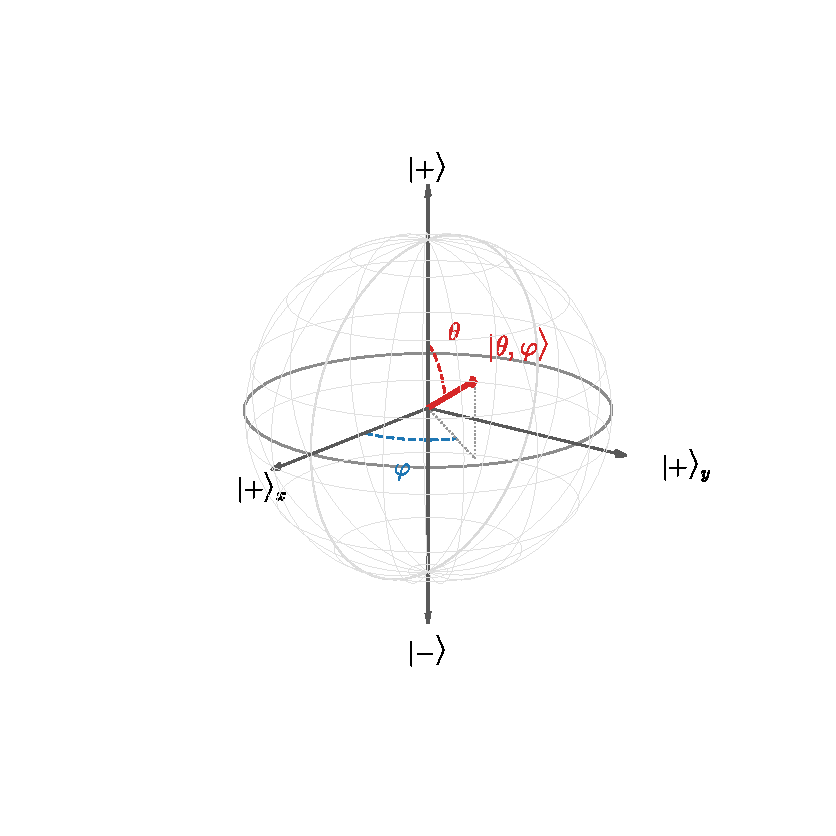
\includegraphics[width=0.56\textwidth]{fig_bloch.pdf}
  \caption{The \emph{pure-state} Bloch sphere: the states
  \eqref{eq:bloch-state} of a spin-$\tfrac12$ system, mapped to unit
  vectors by the exact correspondence $\langle\vec S\rangle =
  \tfrac\hbar2(\sin\theta\cos\varphi, \sin\theta\sin\varphi,
  \cos\theta)$. Poles: the $S_z$ eigenstates; equator at $\varphi =
  0$: the $S_x$ eigenstate $\ket+_x$. Antipodal points --- and only
  antipodal points --- are orthogonal: the sphere's geometry encodes
  the Hilbert space's. (This surface is the boundary of a ball;
  Remark~\ref{rem:bloch-ball}.)}
  \label{fig:bloch}
\end{figure}

\begin{remark}[The sphere is the boundary of a ball]\label{rem:bloch-ball}
The name ``Bloch sphere'' refers to a larger object than
Postulate~\ref{post:states} describes. The general state concept
of quantum mechanics --- covering ensembles and subsystems, not just
maximally-known preparations --- is the \emph{density matrix}
$\rho$, and for two levels every such object is
\begin{equation}
  \rho = \tfrac12\bigl(\idop + \vec r\cdot\vec\sigma\bigr),
  \qquad |\vec r\,| \le 1 ,
\end{equation}
one point of the solid \emph{Bloch ball} per state. Purity is the
boundary condition: $\rho^2 = \rho \iff |\vec r\,| = 1$, and there
$\vec r = \langle\vec\sigma\rangle$ reproduces exactly the map
of Fig.~\ref{fig:bloch} --- what this document calls a state is the
ball's surface, with the interior (mixed states, the center
$\tfrac12\idop$ the ``knows-nothing'' state) describing situations
where the preparation itself is uncertain. This document works with
pure states throughout and does not develop $\rho$; the machinery
is stated here so the figure is not mistaken for the whole story.
[stated; see Sakurai's treatment of density operators and
ensembles --- density matrices are where quantum mechanics meets
statistical mechanics and decoherence.]
\end{remark}

\begin{example}[Stern--Gerlach made quantitative]\label{ex:SG-quant}
The sequence of \S\ref{sec:classical-failures} can now be computed.
The $S_x$ eigenstates sit on the equator, at
$(\theta, \varphi) = (\tfrac\pi2, 0)$ and $(\tfrac\pi2, \pi)$ in
\eqref{eq:bloch-state}:
\begin{equation}
  \ket\pm_x = \tfrac{1}{\sqrt2}\bigl(\ket+ \pm \ket-\bigr),
  \qquad
  \bigl|{}_x\!\braket{+}{+}\bigr|^{\,2}
  = \Bigl|\tfrac{1}{\sqrt2}\Bigr|^2 = \tfrac12 .
\end{equation}
So: the beam filtered to $\ket+$ splits $50{:}50$ at the $S_x$
magnet; the $\ket+_x$ beam, expressed in the $z$ basis, is an equal
superposition again, and the final $S_z$ magnet splits it
$50{:}50$ --- one quarter of the twice-filtered atoms emerge with
$S_z = -\hbar/2$, the value the first filter had \emph{removed}. The
numbers say what \S\ref{sec:classical-failures} could only gesture
at: measuring $S_x$ prepared an $S_x$ eigenstate, which is not an
$S_z$ eigenstate but a superposition of both --- filtering is
\emph{preparation}, and incompatible preparations overwrite each
other. (What ``measurement prepares eigenstates'' means as a
postulate is \S\ref{sec:measurement}'s opening business.)
\end{example}

\subsection{Composite systems: the tensor product}
\label{sec:tensor-product}

One construction completes the kit. Two systems with spaces
$\mathcal H_1, \mathcal H_2$ compose into one with the \emph{tensor
product} $\mathcal H_1 \otimes \mathcal H_2$: basis kets are pairs
$\ket{a}\otimes\ket{b} \equiv \ket{a, b}$, dimensions
\emph{multiply}, operators of system 1 act as $A \otimes \idop$
(each subsystem's operators ignore the other), and inner products
factorize on product kets. The physically loaded fact is what the
construction contains beyond products: a general vector of
$\mathcal H_1 \otimes \mathcal H_2$ is a superposition of product
kets that need not \emph{be} a product ket --- for two spins,
\begin{equation}
  \tfrac{1}{\sqrt2}\bigl(
    \ket{+,-} - \ket{-,+}
  \bigr)
\end{equation}
assigns neither spin a state of its own. Such states are called
\emph{entangled}, they are the generic case (product states are a
measure-zero subset), and their consequences --- correlations no
classical joint distribution reproduces --- are flagged here and
delivered as a physical specimen in \S\ref{sec:addition}
(Remark~\ref{rem:singlet-entangled}); the outlook's identical
particles are where nature makes the choice of symmetric versus
antisymmetric combinations for us. [stated at flag level; the Bell-inequality
story is real, quantitative, and outside this document's arc.]

\medskip
\noindent
The stage is built. What has not been said is what happens on it
when someone \emph{looks} --- the postulates connecting the
formalism to laboratory statistics, and the inequality that
\S\ref{sec:algebra-consequences} promised to make quantitative.


%=======================================================================
\section{Measurement and Uncertainty}
%=======================================================================
\label{sec:measurement}

The stage of \S\ref{sec:hilbert} connects to laboratory statistics
through two postulates --- what the outcomes are, and what remains
afterward. Both were used, unproved, in
Example~\ref{ex:SG-quant}; this section supplies them, extracts the
algebraic criterion for when two observables tolerate each other,
and converts \S\ref{sec:algebra-consequences}'s qualitative ``no
common eigenvectors'' into the quantitative uncertainty relation ---
derived, then \emph{stress-tested}: the section ends by exhibiting,
with Hall, a state that seems to violate it, and locating the
loophole.

\subsection{The measurement postulates}
\label{sec:postulates-measurement}

\begin{postulate}[Born rule]\label{post:born}
Measuring an observable $A = \sum_a a\,P_a$ (spectral form,
\S\ref{sec:computational-moves}) on a normalized state $\ket\psi$
returns one of the eigenvalues $a$, with probability
\begin{equation}
  \boxed{\;
  P(a) = \bra\psi P_a \ket\psi
  \;}
  \qquad
  \bigl(= |\braket a\psi|^2 \text{ when } a \text{ is
  nondegenerate}\bigr).
  \label{eq:born}
\end{equation}
\end{postulate}

\begin{postulate}[Projection]\label{post:projection}
If the outcome is $a$, the state immediately after the measurement
is
\begin{equation}
  \ket\psi \;\longrightarrow\;
  \frac{P_a\ket\psi}{\sqrt{P(a)}} .
  \label{eq:collapse}
\end{equation}
\end{postulate}

\noindent
Three consistency checks, each one line, each delivering a piece of
\S\ref{sec:computational-moves}:
\begin{itemize}
  \item \textbf{Probabilities sum to one} because the projectors do:
  $\sum_a P(a) = \bra\psi\bigl(\sum_a P_a\bigr)\ket\psi
  = \braket\psi\psi = 1$ --- the resolution of the identity
  \eqref{eq:resolution-identity} \emph{is} the conservation of
  probability, which is the physical reason completeness sat in the
  postulates at all.
  \item \textbf{Measurement is repeatable}: measuring $A$ again on
  the post-measurement state \eqref{eq:collapse} returns $a$ with
  probability $\bra\psi P_a^{\,3}\ket\psi/P(a) = 1$ by idempotence
  --- ``asking twice equals asking once,'' now a law rather than a
  slogan, and exactly the ``filtering is preparation'' that
  Example~\ref{ex:SG-quant} read off the beams.
  \item \textbf{Statistics match}: $\sum_a a\,P(a) =
  \bra\psi A\ket\psi$ --- the expectation value
  \eqref{eq:expectation} is the mean of the Born distribution, as
  \S\ref{sec:computational-moves} promised.
\end{itemize}

\begin{remark}[What the postulates do not say]
\label{rem:measurement-problem}
Equation \eqref{eq:collapse} is a \emph{rule}, not a mechanism: it
does not say what physical process implements the jump, when exactly
``a measurement'' has occurred, or how the linear, deterministic
dynamics of Part II coexists with a nonlinear, stochastic update.
These questions --- the measurement problem, decoherence, the
classical limit of measuring devices --- are genuine, quantitative,
and open in parts; this document uses the postulates as every
working calculation does, and flags the foundations rather
than litigating them. [stated; decoherence theory is where the
modern discussion lives.]
\end{remark}

\subsection{Compatible and incompatible observables}
\label{sec:compatibility}

When can two observables have sharp values together? Exactly when
their operators share an eigenbasis --- and the criterion is the
commutator, closing the loop opened by Stern--Gerlach in
\S\ref{sec:classical-failures}.

\begin{proposition}[Compatibility criterion]
\label{prop:compatibility}
Two Hermitian operators with $[A, B] = 0$ possess a common
orthonormal eigenbasis, and conversely.
\end{proposition}

\begin{proof}[Proof (nondegenerate case, displayed; general case
stated)]
Let $A\ket a = a\ket a$ with $a$ nondegenerate. Then
\begin{equation}
  A\,\bigl(B\ket a\bigr)
  = B\,A\ket a
  = a\,\bigl(B\ket a\bigr) :
\end{equation}
$B\ket a$ is again an $a$-eigenvector of $A$, hence (nondegeneracy)
proportional to $\ket a$ --- which says $B\ket a = b\ket a$: the
$A$-eigenbasis already diagonalizes $B$. The converse is immediate
(diagonal matrices commute). [Degenerate case: diagonalize $B$
within each $A$-eigenspace; Sakurai's compatible-observables
discussion runs the induction.]
\end{proof}

\noindent
Compatible observables can be measured in either order with the same
statistics, and their eigenvalues can label states jointly --- the
practice, formalized as a \emph{complete set of commuting
observables} (CSCO), of naming a state by the full list of sharp
quantum numbers it carries. The hydrogen atom's $\ket{n, \ell, m}$
(\S\ref{sec:hydrogen}) is the series' destination example.
Incompatible observables are the interesting ones:
$[S_z, S_x] = \ii\hbar\, S_y \ne 0$, and the Stern--Gerlach
overwriting of \S\ref{sec:classical-failures} now has its one-line
algebraic diagnosis. How \emph{much} incompatibility costs is the
next subsection's theorem.

\subsection{Derivation of the uncertainty relation}
\label{sec:uncertainty}

\begin{theorem}[Robertson]\label{thm:robertson}
For Hermitian $A, B$ and a normalized state $\ket\psi$ (in the
domains of the operators involved --- a clause that
Remark~\ref{rem:uncertainty-counterexample} will show is load-%
bearing),
\begin{equation}
  \boxed{\;
  \Delta A\;\Delta B
  \;\ge\;
  \tfrac12\,\bigl|\bra\psi\,[A, B]\,\ket\psi\bigr| .
  \;}
  \label{eq:robertson}
\end{equation}
\end{theorem}

\begin{proof}
Center the operators: $\bar A \equiv A - \langle A\rangle$,
$\bar B \equiv B - \langle B\rangle$, so that
$(\Delta A)^2 = \|\bar A\ket\psi\|^2$ by \eqref{eq:variance}, and
note the shifts cancel inside the commutator,
$[\bar A, \bar B] = [A, B]$. Cauchy--Schwarz on the two vectors
$\bar A\ket\psi$, $\bar B\ket\psi$:
\begin{equation}
  (\Delta A)^2 (\Delta B)^2
  = \|\bar A\ket\psi\|^2\,\|\bar B\ket\psi\|^2
  \;\ge\;
  \bigl|\bra\psi \bar A\,\bar B\ket\psi\bigr|^2 .
  \label{eq:CS-step}
\end{equation}
Split the product into its Hermitian and anti-Hermitian parts,
\begin{equation}
  \bar A \bar B
  = \tfrac12\{\bar A, \bar B\}
  + \tfrac12[\bar A, \bar B],
\end{equation}
whose expectation values are respectively real and purely imaginary
(the anticommutator of Hermitians is Hermitian; the commutator,
anti-Hermitian --- the same computation as in
\S\ref{sec:brackets-commutators}'s ``the $\ii$'' note). A complex
number's modulus dominates its imaginary part:
\begin{equation}
  \bigl|\bra\psi\bar A\bar B\ket\psi\bigr|^2
  = \tfrac14\,\bigl\langle\{\bar A, \bar B\}\bigr\rangle^2
  + \tfrac14\,\bigl|\bigl\langle[A, B]\bigr\rangle\bigr|^2
  \;\ge\;
  \tfrac14\,\bigl|\bigl\langle[A, B]\bigr\rangle\bigr|^2 ,
  \label{eq:decompose-step}
\end{equation}
and chaining \eqref{eq:CS-step}--\eqref{eq:decompose-step} and
taking square roots gives \eqref{eq:robertson}. (Keeping the
anticommutator term instead of discarding it strengthens the bound
to the \emph{Schr\"odinger} inequality; the discarded term measures
the $A$--$B$ correlations in the state.)
\end{proof}

\noindent
Feed the canonical pair to the theorem: $[\op q, \op p] =
\ii\hbar\,\idop$ has a \emph{state-independent} expectation, so
\begin{equation}
  \boxed{\;
  \Delta q\;\Delta p \;\ge\; \frac{\hbar}{2}
  \;}
  \label{eq:heisenberg}
\end{equation}
for every state in the operators' domains (the theorem's
parenthetical clause rides along) --- the quantitative flesh on
\S\ref{sec:algebra-consequences}'s skeleton, with the classical
limit visible in the formula: the floor under the statistics is set
by exactly the deformation parameter of
Convention~\ref{conv:hbar}. For non-canonical pairs the right-hand
side is an expectation value and therefore \emph{state-dependent}:
\begin{equation}
  \Delta S_x\,\Delta S_y \;\ge\; \tfrac\hbar2\,
  \bigl|\langle S_z\rangle\bigr| ,
  \label{eq:spin-uncertainty}
\end{equation}
a weaker-looking statement with a physical point --- there exist
states ($\langle S_z\rangle = 0$, anywhere on the Bloch equator)
where nothing prevents sharp $S_x$ \emph{and} $S_y$ statistics from
coexisting in the bound, and the bound correctly goes slack.

\begin{example}[The pole saturates]\label{ex:spin-saturation}
Run \eqref{eq:spin-uncertainty} on the laboratory. In the state
$\ket+$ (north pole of Fig.~\ref{fig:bloch}): the Pauli identity
\eqref{eq:pauli-algebra} gives $S_x^2 = S_y^2 = \tfrac{\hbar^2}4
\idop$, while $\langle S_x\rangle = \langle S_y\rangle = 0$ (the
matrices \eqref{eq:pauli} are purely off-diagonal). So
\begin{equation}
  \Delta S_x = \Delta S_y = \frac\hbar2,
  \qquad
  \Delta S_x\,\Delta S_y = \frac{\hbar^2}{4}
  = \frac\hbar2\,\bigl|\langle S_z\rangle\bigr| :
\end{equation}
the inequality is \emph{saturated} --- the spin-up state is a
minimum-uncertainty state of the transverse pair, its unavoidable
transverse spread exactly the floor the algebra charges for a sharp
$S_z$. (Geometrically: a Bloch vector pinned to the pole has its
transverse components maximally undetermined --- the sphere picture
and the algebra agree.)
\end{example}

\paragraph{What saturation requires in general.} Equality in
\eqref{eq:robertson} needs equality at both inequalities of the
proof: Cauchy--Schwarz collapses only when the two vectors are
parallel, $\bar B\ket\psi = c\,\bar A\ket\psi$, and the discarded
anticommutator term vanishes only when
$\operatorname{Re} c = 0$ (substitute the parallelism into
$\langle\{\bar A,\bar B\}\rangle = 2\operatorname{Re}(c)\,
(\Delta A)^2$). Hence the \emph{minimum-uncertainty condition}:
\begin{equation}
  \bigl(\bar B - \ii\lambda\,\bar A\bigr)\ket\psi = 0,
  \qquad \lambda \in \R .
  \label{eq:min-uncertainty-condition}
\end{equation}
For the canonical pair this is a first-order equation whose solution
requires a representation to solve in --- an IOU:
\S\ref{sec:position-momentum} builds the position representation,
solves \eqref{eq:min-uncertainty-condition} there in two lines, and
finds the Gaussian wave packet: \emph{the} state, unique up to
translations, that sits exactly on the floor
\eqref{eq:heisenberg}.

\begin{remark}[Interpretive care: preparation statistics versus disturbance]
\label{rem:ensembles-not-disturbance}
Everything in \eqref{eq:robertson} refers to \emph{preparation
statistics}: $\Delta A$ and $\Delta B$ are standard deviations of
outcome distributions over many runs on identically prepared
systems, each run measuring \emph{one} observable. The theorem says
incompatible statistics cannot both be sharp \emph{in the same
preparation} --- it does not, by itself, quantify how measuring $A$
disturbs a subsequent measurement of $B$ on the same system
(Heisenberg's original microscope heuristic). The disturbance
question is real physics with its own modern formulations, and
conflating the two readings is a standard misstatement of the
uncertainty principle. [stated; error--disturbance
relations are a living literature.]
\end{remark}

\begin{remark}[The counterexample and where the proof leans]
\label{rem:uncertainty-counterexample}
Now the stress test, following Hall \S12.2. Work on
$L^2[-1, 1]$ with the bounded ``position'' $A\psi(x) = x\,\psi(x)$
and the ``momentum'' $B = -\ii\hbar\,\dd/\dd x$ on continuously
differentiable functions with \emph{periodic} boundary values
$\psi(-1) = \psi(1)$ --- a legitimate, essentially self-adjoint
operator (its eigenvectors $\psi_n = \ee^{\ii\pi n x}/\sqrt2$,
$n \in \mathbb Z$, form an orthonormal basis). On a dense domain
one checks $AB - BA = \ii\hbar$, exactly the canonical value. Yet
take $\ket\psi = \psi_n$: it is an eigenvector of $B$, so
$\Delta B = 0$, while $\Delta A$ is finite --- and
\begin{equation}
  \Delta A\;\Delta B = 0 \;<\; \frac\hbar2\;,
\end{equation}
an apparent violation. The resolution is the parenthetical clause of
Theorem~\ref{thm:robertson}: the proof applies $B$ after $A$, and
$A\psi_n = x\,\psi_n$ \emph{violates the periodic boundary
condition} ($x\,\psi_n$ takes different values at $\pm1$), so
$\psi_n \notin \operatorname{Dom}(BA)$ --- the state sits exactly
outside the hypotheses, and the inequality never applied to it. Two
morals, one local, one global. Local: the physical system here is a
particle on a \emph{ring}, $A$ is (essentially) an angle and $B$ an
angular momentum, and the lesson is that a bounded, periodic
coordinate admits no naive uncertainty relation with its conjugate
momentum --- a fact that returns, constructively, when
\S\ref{sec:J-spectrum} builds angular momentum. Global: this is the
promised second bite of Remark~\ref{rem:self-adjoint-pothole} ---
domains are not decoration, and the hypotheses of a theorem
are part of its physics. [Example verified against Hall \S12.2.]
\end{remark}

\medskip
\noindent
Kinematics still lacks its most-used representation: the one in
which states are \emph{functions}, $\psi(x)$, and
\eqref{eq:min-uncertainty-condition} becomes a differential
equation. Building it --- and deriving
$\op p = -\ii\hbar\,\partial_x$ within it --- is the next section's
business.


%=======================================================================
\section{Position, Momentum, and Translation}
%=======================================================================
\label{sec:position-momentum}

Kinematics closes with its most-used representation: states as
functions. Building it means confronting an operator whose spectrum
is a continuum --- which imports the delta
apparatus of the field-theory notes --- and the payoff is
structural: the canonical commutator, \emph{postulated} in
\S\ref{sec:brackets-commutators} as a deformation of the classical
bracket, will here be \emph{derived} a second, independent way, from
the geometry of translations. Two roads, one commutator; their
convergence is the first entry of the quantum Noether dictionary.

\subsection{The position basis and its fine print}
\label{sec:position-basis}

A particle on a line has a position operator $\op q$ whose possible
sharp values fill $\R$: a continuous spectrum. Write formal
eigenkets $\op q\ket x = x\ket x$ and trade
Theorem~\ref{thm:spectral}'s sums for integrals, replacing the
Kronecker delta of orthonormality by its continuum original:
\begin{equation}
  \braket{x'\!}{x} = \delta(x - x'),
  \qquad
  \boxed{\;
  \idop = \int \dd x\; \ket x\bra x .
  \;}
  \label{eq:position-completeness}
\end{equation}
The delta function arrives with the license already issued in
[Fld.\ \S10.2, App.~B]: not a function but a distribution, every
manipulation below the shadow of a legitimate operation on smeared
objects --- the identical fiction, imported wholesale. The fine
print: $\ket x$ itself is \emph{not} a vector of the Hilbert space
(its ``norm'' is $\delta(0)$); it is a computational scaffold, and
the physically meaningful objects are the coefficients it produces,
\begin{equation}
  \psi(x) \equiv \braket x\psi ,
  \qquad
  \braket\psi\psi = \int\dd x\,\bigl|\psi(x)\bigr|^2 = 1 ,
\end{equation}
--- the \emph{wavefunction}: the state's components in the position
basis, exactly as $\braket a\psi$ were its components in a discrete
one. Born's rule \eqref{eq:born} reads through the trade: with no
normalizable eigenvector, $|\psi(x)|^2$ is a probability
\emph{density}, its integral over a region the probability of
finding the particle there. [The mathematically clean route is the
spectral theorem without eigenvectors, Hall Ch.\ 10; rigged Hilbert
spaces legitimizing $\ket x$ directly are a second route, outside
Hall; stated, and the working
notation is safe for everything this document does.]

\subsection{Translation and the operator it generates}
\label{sec:translation}

Now the geometry. Define the \emph{translation operator} by its
action on the position basis,
\begin{equation}
  T(a)\,\ket x = \ket{x + a},
\end{equation}
extended by linearity. It is unitary (it maps the orthonormal
continuum \eqref{eq:position-completeness} onto itself), composes as
the line's additive group, $T(a)\,T(b) = T(a + b)$, $T(0) = \idop$,
and carries one commutator on its face: on any basis ket,
\begin{equation}
  \op q\,T(a)\ket x = (x + a)\ket{x+a},
  \qquad
  T(a)\,\op q\ket x = x\ket{x+a}
  \qquad\Longrightarrow\qquad
  [\op q,\, T(a)] = a\,T(a) .
  \label{eq:q-T-commutator}
\end{equation}
Look at an infinitesimal translation. Unitarity and smoothness force
the form
\begin{equation}
  T(\dd a)
  = \idop - \frac{\ii}{\hbar}\,\op p\;\dd a + O(\dd a^2),
  \label{eq:generator-def}
\end{equation}
which \emph{defines} an operator $\op p$ --- the \emph{generator} of
translations --- Hermitian because $T$ is unitary (expand
$T^\dagger T = \idop$ to first order: $\op p^\dagger = \op p$), with
the $\hbar$ inserted so that $[\op p] = [\text{action}]/[\text{%
length}] = [\text{momentum}]$: the name is a promise, about
to be kept. Insert \eqref{eq:generator-def} into
\eqref{eq:q-T-commutator} and keep first order:
\begin{equation}
  -\frac{\ii}{\hbar}\,[\op q, \op p]\;\dd a
  = \dd a\;\idop
  \qquad\Longrightarrow\qquad
  \boxed{\;
  [\op q, \op p] = \ii\hbar\,\idop .
  \;}
  \label{eq:CCR-derived}
\end{equation}

\begin{remark}[Two roads to one commutator: the quantum Noether
dictionary]\label{rem:quantum-noether}
Equation \eqref{eq:CCR-derived} is the canonical commutation
relation \eqref{eq:CCR} again --- reached by a completely different
road. Section~\ref{sec:brackets-commutators} \emph{deformed} the
classical bracket ($\{q, p\} = 1$, Dirac's rule); this section never
mentioned a bracket, only the statement \emph{``$\op p$ is what
translates.''} That the two roads meet is not a coincidence to
admire but a dictionary to use: in mechanics, Noether traded each
symmetry for a conserved quantity, and momentum \emph{was} the
translation entry [Mech.\ \S3.3], as it was again for fields
[Fld.\ \S9.4]. Quantum mechanics keeps the trade and sharpens it:
\emph{the conserved quantity is the symmetry's generator}, as an
operator ---
\begin{center}
\begin{tabular}{lll}
\toprule
symmetry & generator & where \\
\midrule
spatial translation & $\op p$ & here \\
time translation & $\op H$ & \S\ref{sec:evolution} \\
rotation & $\op J_i$ & \S\ref{sec:rotations} \\
\bottomrule
\end{tabular}
\end{center}
--- and the commutators among generators are the transcription of
the classical bracket algebra, one theorem per row ahead.
\end{remark}

\subsection{$\op p$ in the position representation}
\label{sec:p-position-rep}

What does $\op p$ do to wavefunctions? Compute
$\bra x T(\dd a)\ket\psi$ twice. Geometrically: acting leftward,
$\bra x T(\dd a) = \bra{x - \dd a}$ (the adjoint of
$T(\dd a)\ket x = \ket{x + \dd a}$, since $T^\dagger(\dd a) =
T(-\dd a)$), so
\begin{equation}
  \bra x T(\dd a)\ket\psi
  = \psi(x - \dd a)
  = \psi(x) - \dd a\,\pd\psi x + O(\dd a^2).
\end{equation}
Algebraically, via \eqref{eq:generator-def}:
$\bra x T(\dd a)\ket\psi = \psi(x) - \tfrac\ii\hbar\,\dd a\,
\bra x\op p\ket\psi$. Equate the first orders:
\begin{equation}
  \boxed{\;
  \bra x\,\op p\,\ket\psi
  = -\,\ii\hbar\,\pd{}{x}\,\psi(x)
  \;}
  \label{eq:p-position}
\end{equation}
--- the textbook formula for momentum: here not a postulate
but the unique answer to ``what must the translation
generator look like on functions that get dragged.'' Hermiticity in
this representation is one integration by parts,
$\int\psi_1^{*}(-\ii\hbar\,\partial_x\psi_2)\,\dd x =
\int(-\ii\hbar\,\partial_x\psi_1)^{*}\psi_2\,\dd x$ + boundary
terms --- and the boundary terms are precisely where the potholes of
Remarks~\ref{rem:self-adjoint-pothole} and
\ref{rem:uncertainty-counterexample} lived: on the full line with
decay they vanish and all is well; on intervals, they were the whole
story.

The eigenvalue problem of \eqref{eq:p-position} is immediate:
$-\ii\hbar\,\partial_x\braket xp = p\braket xp$ gives
\begin{equation}
  \braket xp
  = \frac{1}{\sqrt{2\pi\hbar}}\;
    \ee^{\ii p x/\hbar},
  \qquad
  \braket{p'\!}p
  = \frac{1}{2\pi\hbar}\int\dd x\;
    \ee^{\ii(p - p')x/\hbar}
  = \delta(p - p')
  \label{eq:momentum-eigenstate}
\end{equation}
(the normalization check is the Fourier representation of the
delta: the $\sigma \to \infty$ limit of the Gaussian pair
\eqref{eq:gaussian-fourier}, read distributionally under the license
of [Fld.\ App.~B]). A momentum eigenstate is a plane wave
of wavelength
\begin{equation}
  \lambda = \frac{2\pi\hbar}{p} = \frac{h}{p}
\end{equation}
--- de Broglie's relation, here neither postulate nor analogy but
the shape of the translation generator's eigenfunctions.

\subsection{The momentum representation and the Fourier bridge}
\label{sec:momentum-rep}

The momentum eigenkets are delta-normalized and complete in their
own right, so a state has momentum-basis components
$\varphi(p) \equiv \braket p\psi$, and the bridge between the two
descriptions is one insertion of
\eqref{eq:position-completeness}:
\begin{equation}
  \varphi(p)
  = \int\dd x\;\braket px\,\braket x\psi
  = \int\frac{\dd x}{\sqrt{2\pi\hbar}}\;
    \ee^{-\ii p x/\hbar}\,\psi(x)
  \label{eq:fourier-bridge}
\end{equation}
--- the Fourier transform, with its inverse running the other way.
This is Remark~\ref{rem:adapted-coordinates-qm} delivered in
full: position and momentum representations are the two adapted
coordinate systems ($\op q$ diagonal versus $\op p$ diagonal), the
change between them is a basis change like any other, and the
celebrated transform is nothing but
$\braket px$ used as a transition matrix. In the momentum
representation the roles swap symmetrically: $\op p$ multiplies and
$\bra p\op q\ket\psi = +\ii\hbar\,\partial_p\varphi(p)$ (same
derivation, sign from conjugating \eqref{eq:momentum-eigenstate}).

\subsection{The Gaussian minimum-uncertainty packet}
\label{sec:gaussian-packet}

Section~\ref{sec:uncertainty} left one item open: the
minimum-uncertainty
condition \eqref{eq:min-uncertainty-condition}, waiting for a
representation to be solved in. In the position representation,
with $\bar p = \op p - p_0$ and $\bar q = \op q - x_0$
(expectations $p_0, x_0$), the condition
$(\bar p - \ii\lambda\bar q)\ket\psi = 0$ reads
\begin{equation}
  \Bigl(
    -\ii\hbar\,\pd{}{x} - p_0
    - \ii\lambda\,(x - x_0)
  \Bigr)\,\psi(x) = 0
  \qquad\Longrightarrow\qquad
  \pd\psi x
  = \Bigl[
      \frac{\ii p_0}{\hbar}
      - \frac{\lambda}{\hbar}(x - x_0)
    \Bigr]\psi ,
\end{equation}
a first-order linear equation with a two-line solution:
\begin{equation}
  \boxed{\;
  \psi(x)
  = N\,
    \exp\!\Bigl[
      \frac{\ii p_0 x}{\hbar}
      \;-\;
      \frac{(x - x_0)^2}{4(\Delta x)^2}
    \Bigr],
  \qquad
  (\Delta x)^2 = \frac{\hbar}{2\lambda} ,
  \;}
  \label{eq:gaussian-packet}
\end{equation}
normalizable precisely when $\lambda > 0$, with the variance read
off the profile
$|\psi|^2 \propto \exp[-(x-x_0)^2/2(\Delta x)^2]$
(integrals: Appendix~\ref{app:gaussians}). No further computation is needed for
the momentum spread: the state was \emph{constructed} to saturate,
so $\Delta p = \hbar/(2\,\Delta x)$ by Theorem~\ref{thm:robertson}'s
equality case --- and the direct check confirms it: the Fourier
bridge \eqref{eq:fourier-bridge} of a Gaussian is again a Gaussian
(Appendix~\ref{app:gaussians}), with exactly the reciprocal width.
\emph{The Gaussian wave packet is the unique family of states
sitting on the floor} $\Delta x\,\Delta p = \hbar/2$
(Fig.~\ref{fig:wavepacket}): squeeze the left panel and the right
panel broadens in exact compensation, the deformation parameter
$\hbar$ fixing the product.

\begin{figure}[htbp]
  \centering
  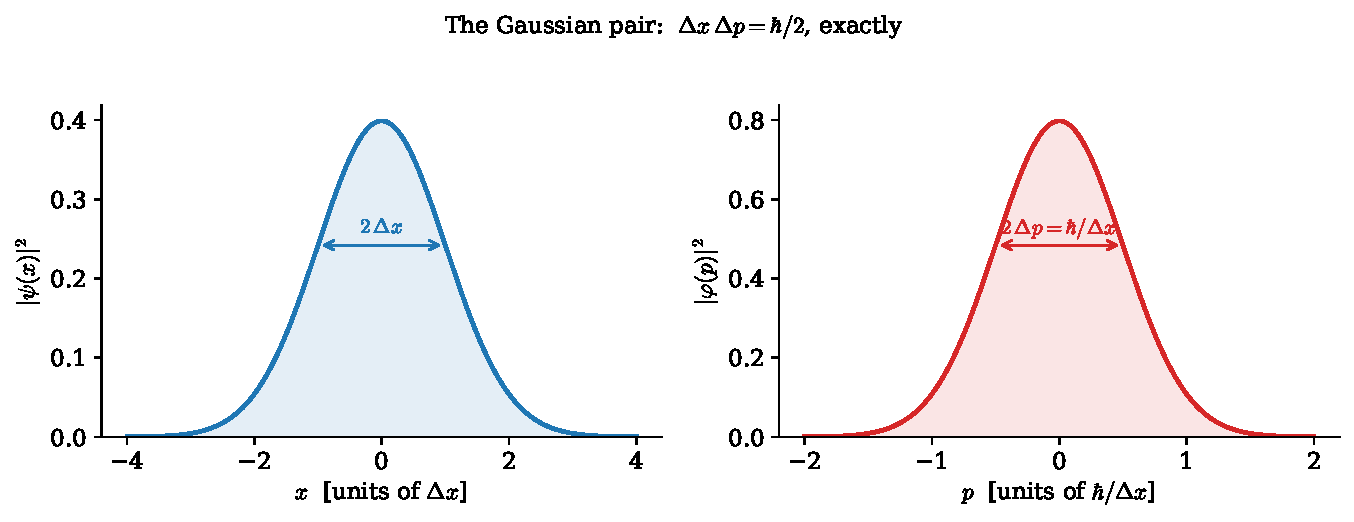
\includegraphics[width=0.94\textwidth]{fig_wavepacket.pdf}
  \caption{The minimum-uncertainty state
  \eqref{eq:gaussian-packet} in both adapted coordinate systems,
  drawn from the exact formulas ($\hbar = 1$, $\Delta x = 1$,
  $x_0 = p_0 = 0$). The widths are reciprocal,
  $\Delta p = \hbar/(2\Delta x)$: narrowing the position
  distribution forces a wider momentum distribution, the product
  fixed at $\Delta x\,\Delta p = \hbar/2$.}
  \label{fig:wavepacket}
\end{figure}

\begin{example}[Why atoms are the size they are]
\label{ex:atomic-size}
The uncertainty floor is not philosophy; it is a pressure, and it
holds atoms up --- answering the first puzzle of
\S\ref{sec:classical-failures}. Confine an electron to an
atomic length, $\Delta x \approx 0.5\,\text{\AA} =
5\times10^{-11}\,\mathrm m$. The floor \eqref{eq:heisenberg} forces
\begin{equation}
  p \;\gtrsim\; \frac{\hbar}{2\,\Delta x}
  \approx 1.1\times10^{-24}\,\mathrm{kg\,m/s}
  \qquad\Longrightarrow\qquad
  E_{\text{kin}} \sim \frac{p^2}{2m_e}
  \approx 6.1\times10^{-19}\,\mathrm J
  \approx 3.8\,\mathrm{eV} :
\end{equation}
electron-volt-scale kinetic energy, forced by localization alone
--- the atomic energy scale, from nothing but $\hbar$, $m_e$, and a
length. Squeezing the electron further toward the nucleus raises
this cost as $1/(\Delta x)^2$, faster than the Coulomb energy
$\sim -1/\Delta x$ can compensate; the balance point \emph{is} the atom,
and the classical spiral-in of
\S\ref{sec:classical-failures} is arrested by the same inequality
drawn in Fig.~\ref{fig:wavepacket}. (The balance is made exact, with
the numerical constant earned, at the hydrogen capstone of
\S\ref{sec:hydrogen}.)
\end{example}

\medskip
\noindent
Part I is complete: an algebra (\S\ref{sec:brackets-commutators}), a
stage (\S\ref{sec:hilbert}), measurement rules
(\S\ref{sec:measurement}), and coordinates
(\S\ref{sec:position-momentum}). Nothing yet \emph{moves}. Part II
turns on time --- and the first thing it will do is run the quantum
Noether dictionary's second row.


%=======================================================================
\clearpage
\part{Dynamics}
%=======================================================================

%=======================================================================
\section{Time Evolution}
%=======================================================================
\label{sec:evolution}

Nothing in Part I moved. This section turns on time, and the
structure is deliberately a rerun: exactly as \S\ref{sec:translation}
derived the momentum operator from ``something must implement
spatial shifts,'' here the Hamiltonian is derived from ``something
must implement waiting'' --- which fills the second
row of the quantum Noether dictionary
(Remark~\ref{rem:quantum-noether}). The
section ends where quantum dynamics always ends: in the energy
eigenbasis, where the whole of time evolution is a set of rotating
phases --- and with the series' laboratory precessing on the Bloch
sphere --- the working principle of MRI.

\subsection{The evolution operator and where $H$ comes from}
\label{sec:evolution-operator}

Let $\ket{\psi(t)}$ be the state at time $t$ of a system prepared as
$\ket{\psi(0)}$. Two physical requirements pin down the map between
them:
\begin{itemize}
  \item \textbf{Probability is conserved}: $\braket{\psi(t)}{\psi(t)}
  = 1$ at all times, for every initial state --- the map
  $U(t)$ with $\ket{\psi(t)} = U(t)\ket{\psi(0)}$ must be
  \emph{unitary} (\S\ref{sec:operators}: unitaries are exactly the
  inner product's isometries).
  \item \textbf{Waiting composes}: evolving for $t_1$ and then $t_2$
  is evolving for $t_1 + t_2$, and no moment is special (a closed
  system; explicit time dependence would encode an outside agent):
  $U(t_2)\,U(t_1) = U(t_1 + t_2)$, $U(0) = \idop$.
\end{itemize}
These are verbatim the properties that \S\ref{sec:translation} used
for spatial shifts --- a one-parameter unitary group, now in time
--- so the same move applies: expand the infinitesimal element,
\begin{equation}
  U(\dd t)
  = \idop - \frac{\ii}{\hbar}\,\op H\,\dd t + O(\dd t^2),
  \label{eq:H-generator}
\end{equation}
which \emph{defines} a Hermitian operator $\op H$ --- the generator
of time translations --- with $\hbar$ inserted so that
$[\op H] = [\text{action}]/[\text{time}] = [\text{energy}]$. The
name \emph{Hamiltonian} is the dictionary's second row: in mechanics,
the conserved quantity guaranteed by time-translation invariance
\emph{was} the Hamiltonian [Mech.\ \S\S3.3, 6.2], and quantum
mechanics
promotes that conserved quantity to the generator itself. [That
every strongly continuous one-parameter unitary group has such a
self-adjoint generator is Stone's theorem --- Hall \S10.2; stated,
and it is the precise justification for \eqref{eq:H-generator}.]

Differentiate the composition law at finite $t$ --- or simply apply
\eqref{eq:H-generator} to $U(t + \dd t) = U(\dd t)\,U(t)$ --- to get
the operator equation and its state-level shadow:
\begin{equation}
  \boxed{\;
  \ii\hbar\,\pd{}{t}\,U(t) = \op H\,U(t),
  \qquad
  \ii\hbar\,\pd{}{t}\,\ket{\psi(t)} = \op H\,\ket{\psi(t)}
  \;}
  \label{eq:schrodinger}
\end{equation}
--- the \emph{Schr\"odinger equation}, obtained here as the
differential form of ``waiting is unitary and composes,'' with all
its famous features inherited rather than postulated: linear
(because $U$ is), probability-conserving (because $U$ is), and
first order in time (because groups have one-parameter tangents).
For an $\op H$ with no explicit time dependence the solution
closes:
\begin{equation}
  U(t) = \exp\!\Bigl[-\frac{\ii\,\op H\,t}{\hbar}\Bigr].
  \label{eq:U-exponential}
\end{equation}
(Sandwiching \eqref{eq:schrodinger} in the position basis, with the
Hamiltonian $\op p^2/2m + V(\op q)$ and the representation
\eqref{eq:p-position}, produces the wave equation
$\ii\hbar\,\partial_t\psi = -\tfrac{\hbar^2}{2m}\partial_x^2\psi +
V\psi$ --- the form \S\ref{sec:one-dim} will live in.)

\subsection{The energy eigenbasis: dynamics is phases}
\label{sec:stationary-states}

Now the adapted-coordinates discipline
(Remark~\ref{rem:adapted-coordinates-qm}), fourth appearance ---
and its most consequential. Diagonalize the operator that generates the
dynamics: $\op H\ket n = E_n\ket n$. In this basis
\eqref{eq:U-exponential} is diagonal, and every initial state
evolves by
\begin{equation}
  \boxed{\;
  \ket{\psi(t)}
  = \sum_n c_n\;\ee^{-\ii E_n t/\hbar}\,\ket n,
  \qquad
  c_n = \braket n{\psi(0)} :
  \;}
  \label{eq:phase-evolution}
\end{equation}
\emph{the entire dynamics of quantum mechanics is a set of rotating
phases}, one per energy level, at rates set by the spectrum. Solving
a quantum system \emph{means} finding the spectrum; everything after
is \eqref{eq:phase-evolution}. Two immediate consequences, one per
extreme:
\begin{itemize}
  \item \textbf{One term: stationary states.} An energy eigenstate
  evolves as $\ee^{-\ii E_n t/\hbar}\ket n$ --- an overall phase,
  physically empty (\S\ref{sec:kets}): every probability, every
  expectation value is frozen. Here, at last, is the full answer to
  \S\ref{sec:classical-failures}'s stability crisis: an atom in its
  ground state is not an electron \emph{orbiting} --- not a charge
  accelerating, not a system doing anything --- it is a stationary
  state, and stationary states have no dynamics to radiate away.
  \item \textbf{Two terms: beats at the Bohr frequency.} A
  superposition $c_1\ket 1 + c_2\ket 2$ has one \emph{relative}
  phase --- physical (\S\ref{sec:kets}) --- rotating at
  \begin{equation}
    \omega_{21} = \frac{E_2 - E_1}{\hbar},
    \label{eq:bohr-frequency}
  \end{equation}
  so every observable connecting the two levels oscillates at
  $\omega_{21}$: the quantum system \emph{beats}, exactly as two
  coupled classical modes did [Osc.\ \S6.6], with energy differences
  playing the role of frequency differences. This is why atoms emit
  \emph{lines} and why the lines sit at differences of a fixed set
  of terms (the Rydberg--Ritz combination principle, mysterious in
  1908, one line in \eqref{eq:bohr-frequency}): this answers the second
  experimental puzzle of \S\ref{sec:classical-failures} in structure;
  the numbers arrive at the hydrogen capstone. [One gap,
  flagged: an atom \emph{prepared} in an excited stationary state
  also radiates --- spontaneous emission --- which no isolated-atom
  stationary state can explain; the mechanism is the coupling to the
  quantized field of the outlook, and the beat picture above is its
  semiclassical face. Stated.]
\end{itemize}

\subsection{The laboratory precesses: spin in a magnetic field}
\label{sec:precession}

Run the machinery end to end on the two-state laboratory. A
spin-$\tfrac12$ magnetic moment in a uniform field $\vec B = B\hat z$
has
\begin{equation}
  \op H = -\gamma B\,\op S_z,
  \qquad
  E_\pm = \mp\,\frac{\gamma\hbar B}{2},
  \qquad
  \omega \equiv \frac{E_- - E_+}{\hbar} = \gamma B
\end{equation}
($\gamma$ the gyromagnetic ratio; the $S_z$ eigenstates are the
stationary states, and $\omega$ is the Bohr frequency of the only
pair there is). Prepare the state at the equator,
$\ket{\psi(0)} = \ket+_x = (\ket+ + \ket-)/\sqrt2$, and apply
\eqref{eq:phase-evolution}:
\begin{equation}
  \ket{\psi(t)}
  = \frac{1}{\sqrt2}\Bigl(
      \ee^{\ii\omega t/2}\,\ket+
      + \ee^{-\ii\omega t/2}\,\ket-
    \Bigr),
\end{equation}
which is the Bloch state \eqref{eq:bloch-state} with
$\theta = \tfrac\pi2$, $\varphi = -\omega t$: the expectation
vector,
\begin{equation}
  \langle S_x\rangle = \tfrac\hbar2\cos\omega t,
  \qquad
  \langle S_y\rangle = -\tfrac\hbar2\sin\omega t,
  \qquad
  \langle S_z\rangle = 0,
\end{equation}
\emph{precesses} around the field at the \emph{Larmor frequency}
$\omega = \gamma B$ --- uniform circular motion of the Bloch vector
on the equator of Fig.~\ref{fig:bloch}: the figure of
\S\ref{sec:spin-half}, now a movie.

\begin{example}[Larmor precession in the clinic: MRI]
\label{ex:mri}
For a proton, $\gamma_p/2\pi = 42.58\,\mathrm{MHz/T}$
[experimental input; CODATA]. In the
$3\,\mathrm T$ field of a clinical MRI magnet, the hydrogen nuclei
of the body's water precess at
\begin{equation}
  f = \frac{\gamma_p B}{2\pi}
  = 42.58\,\mathrm{MHz/T} \times 3\,\mathrm T
  \approx 128\,\mathrm{MHz}
\end{equation}
--- a radio frequency. An MRI machine is a Larmor-precession
transceiver: it tips the protons' Bloch vectors off axis, listens
for the $128\,\mathrm{MHz}$ signal of their collective precession,
and maps tissue by how the precession decays. A clinical scan
is Eq.~\eqref{eq:phase-evolution} run on $\sim 10^{27}$ copies of
the two-state laboratory.
\end{example}

\begin{remark}[The $2\pi$ seed]\label{rem:2pi-seed}
Watch the state, not just its expectation vector, through one full
turn. At $t = 2\pi/\omega$ the Bloch vector has returned --- but the
ket has not:
\begin{equation}
  \ket{\psi(2\pi/\omega)}
  = \frac{1}{\sqrt2}\bigl(
      \ee^{\ii\pi}\ket+ + \ee^{-\ii\pi}\ket-
    \bigr)
  = -\,\ket{\psi(0)} :
\end{equation}
a full $2\pi$ of precession multiplies the state by $-1$, and only
$4\pi$ restores it. For an isolated spin the sign is an overall
phase, invisible (\S\ref{sec:kets}) --- but a phase becomes
\emph{relative}, and hence measurable, the moment the spin is one
arm of an interferometer. That experiment exists, with neutrons, and
\S\ref{sec:su2} owes the reader its number; the present remark is
the seed: the $-1$ is not an artifact of this Hamiltonian but the
signature of what kind of representation of the rotation group a
spin-$\tfrac12$ carries.
\end{remark}

\begin{remark}[Energy--time is not Robertson]
\label{rem:energy-time}
A caution the two-level beat invites. There is no time operator to
feed Theorem~\ref{thm:robertson} --- in this formalism $t$ is a
parameter, not an observable [stated; the obstruction to a
self-adjoint time conjugate to a bounded-below $H$ is Pauli's
observation], so ``$\Delta E\,\Delta t \ge \hbar/2$'' cannot mean
what $\Delta q\,\Delta p$ means. The precise version is one line
away. Differentiate an expectation value with
\eqref{eq:schrodinger}:
\begin{equation}
  \tot{}{t}\langle A\rangle
  = \frac{\ii}{\hbar}\,
    \bigl\langle\,[\op H, \op A]\,\bigr\rangle
  \qquad(\text{$A$ with no explicit $t$-dependence}),
  \label{eq:expectation-flow}
\end{equation}
then run Robertson on the pair $(\op A, \op H)$ and substitute:
$\Delta A\,\Delta E \ge \tfrac\hbar2\,|\dd\langle A\rangle/\dd t|$,
i.e.
\begin{equation}
  \Delta E\;\tau_A \;\ge\; \frac{\hbar}{2},
  \qquad
  \tau_A \equiv
  \frac{\Delta A}{\bigl|\dd\langle A\rangle/\dd t\bigr|}
  \label{eq:mandelstam-tamm}
\end{equation}
(Mandelstam--Tamm): $\tau_A$ is the time for the statistics of $A$
to shift by one standard deviation, and the theorem says
\emph{states with sharp energy change slowly} --- the stationary
state ($\Delta E = 0$, nothing moves) is its extreme case, and a
spectral line's width--lifetime relation its laboratory face.
Equation \eqref{eq:expectation-flow} is more than this remark's
tool: it is the quantum mirror of $\dot F = \{F, H\}$ [Mech.\ \S8.2],
about to be promoted from expectation values to the operators
themselves --- which is precisely the next section.
\end{remark}


%=======================================================================
\section{Two Pictures of One Physics}
%=======================================================================
\label{sec:pictures}

Remark~\ref{rem:energy-time} ended mid-promotion: the flow equation
\eqref{eq:expectation-flow} moved \emph{expectation values}, and the
promise was to move the operators themselves. This section keeps it
--- and the payoff, for a reader of the mechanics notes: the quantum equation
of motion \emph{is} the classical bracket flow, transcribed by
Dirac's rule with nothing lost in translation. The section then
locates the classical limit (Ehrenfest), and closes by dissolving a
historical rivalry into a choice of coordinates.

\subsection{The Heisenberg picture: operators flow}
\label{sec:heisenberg-picture}

Everything measurable is a sandwich, and a sandwich has two slices:
\begin{equation}
  \bra{\psi(t)}\,\op A\,\ket{\psi(t)}
  = \bra{\psi(0)}\;
    \underbrace{U^\dagger(t)\,\op A\,U(t)}_{\displaystyle
    \equiv\; \op A_H(t)}
    \;\ket{\psi(0)} .
  \label{eq:picture-split}
\end{equation}
Section~\ref{sec:evolution} attached the evolution to the state (the
\emph{Schr\"odinger picture}); attach it instead to the operator ---
states frozen at $\ket{\psi(0)}$, observables carrying the time ---
and nothing measurable changes, because \eqref{eq:picture-split} is
an identity. This is the \emph{Heisenberg picture}, and its equation
of motion is one derivative away. With $\op H$ time-independent,
$U(t) = \ee^{-\ii\op H t/\hbar}$ commutes with $\op H$, and
differentiating $\op A_H = U^\dagger \op A\, U$ by the product rule
(using \eqref{eq:schrodinger} and its adjoint):
\begin{equation}
  \tot{\op A_H}{t}
  = \frac{\ii}{\hbar}\,U^\dagger\,[\op H, \op A]\,U
  = \frac{\ii}{\hbar}\,[\op H, \op A_H],
\end{equation}
i.e., written to make the point unmissable:
\begin{equation}
  \boxed{\;
  \tot{\op A_H}{t}
  = \frac{1}{\ii\hbar}\,\bigl[\op A_H,\, \op H\bigr]
  \;}
  \qquad\text{versus}\qquad
  \tot Ft = \{F, H\}
  \quad\text{[Mech.\ \S8.2]}.
  \label{eq:heisenberg-eom}
\end{equation}
Dirac's rule \eqref{eq:dirac-rule} was installed in
\S\ref{sec:brackets-commutators} as a statement about
\emph{kinematics} --- replace the bracket's realization, keep its
algebra. Equation \eqref{eq:heisenberg-eom} says the replacement
extends to \emph{dynamics} verbatim: the law of motion is the same
sentence in the new realization. Three corollaries fall out at the
speed of substitution:
\begin{itemize}
  \item \textbf{Conservation is commutation.} $[\op A, \op H] = 0$
  freezes $\op A_H$ for all time --- the quantum Noether loop closes
  at the operator level: the generators of
  Remark~\ref{rem:quantum-noether}'s table are conserved exactly
  when their symmetry is a symmetry \emph{of the dynamics}, and by
  \S\ref{sec:compatibility} the conserved quantities are precisely
  the observables sharable with energy. A CSCO containing $\op H$
  is therefore the natural naming scheme for stationary states ---
  the $(n, \ell, m)$ of the hydrogen capstone are exactly such a
  list.
  \item \textbf{The canonical structure rides along.} Unitary
  conjugation preserves commutators, so
  $[\op q_H(t), \op p_H(t)] = \ii\hbar$ at every (equal) time ---
  the quantum echo of the classical fact that time evolution
  preserves the fundamental brackets [time evolution is the flow
  generated by $H$, Mech.\ \S8.3; that Hamiltonian flows preserve
  the fundamental brackets is part of the canonical-transformation
  theory the mechanics notes' outlook only points to --- stated
  there, proved neither there nor here].
  \item \textbf{The algebra of \S\ref{sec:algebra-consequences} was
  built for this.} The derivative formulas
  \eqref{eq:commutator-derivative} turn \eqref{eq:heisenberg-eom}
  into operator-valued classical mechanics, next.
\end{itemize}

\subsection{Operator Newton: two flows run explicitly}
\label{sec:operator-newton}

\emph{Free particle}, $\op H = \op p^2/2m$: the flow equations
\begin{equation}
  \tot{\op p_H}t = 0,
  \qquad
  \tot{\op q_H}t
  = \frac{1}{\ii\hbar}\Bigl[\op q_H, \frac{\op p_H^2}{2m}\Bigr]
  = \frac{\op p_H}{m}
\end{equation}
(the second by \eqref{eq:commutator-derivative}) integrate to
\begin{equation}
  \op q_H(t) = \op q(0) + \frac{\op p(0)}{m}\,t
  \label{eq:free-trajectory}
\end{equation}
--- the classical trajectory, \emph{as an operator identity}. The
quantum content hides in what the classical formula cannot say:
\begin{equation}
  \bigl[\op q_H(t),\, \op q_H(0)\bigr]
  = \frac{t}{m}\,[\op p(0), \op q(0)]
  = -\,\frac{\ii\hbar\, t}{m}
  \;\ne\; 0 :
  \label{eq:position-noncommute}
\end{equation}
\emph{the position now and the position later are incompatible
observables}. By Theorem~\ref{thm:robertson}, a sharp position at
$t = 0$ forces growing position spread later ---
$\Delta q(t)\,\Delta q(0) \ge \hbar t/2m$ --- which is wave-packet
spreading, obtained with no wavefunction in sight; the
wave-mechanical version, with the full time profile, is
\S\ref{sec:one-dim}'s opening act.

\emph{General potential}, $\op H = \op p^2/2m + V(\op q)$: the same
two lines give
\begin{equation}
  \tot{\op q_H}t = \frac{\op p_H}m,
  \qquad
  \tot{\op p_H}t = -\,V'(\op q_H)
  \qquad\Longrightarrow\qquad
  m\,\frac{\dd^2\op q_H}{\dd t^2} = -\,V'(\op q_H)
  \label{eq:operator-newton}
\end{equation}
--- Newton's second law, wearing hats.

\subsection{Ehrenfest and where the classical world sits}
\label{sec:ehrenfest}

Sandwich \eqref{eq:operator-newton} in the (frozen) state:
\begin{equation}
  m\,\frac{\dd^2}{\dd t^2}\,\langle\op q\rangle
  = -\,\bigl\langle V'(\op q)\bigr\rangle
  \qquad\text{(Ehrenfest)},
  \label{eq:ehrenfest}
\end{equation}
and resist the tempting misreading: the right side is
$-\langle V'(\op q)\rangle$, \emph{not} $-V'(\langle\op q\rangle)$,
and the two differ whenever the packet is wide enough to sample the
potential's curvature --- Taylor-expand about the center,
\begin{equation}
  \bigl\langle V'(\op q)\bigr\rangle
  = V'(\langle q\rangle)
  + \tfrac12\,V'''(\langle q\rangle)\,(\Delta q)^2 + \cdots ,
\end{equation}
so the center of a quantum state obeys classical mechanics exactly
when (i) the potential is at most quadratic --- $V''' = 0$: the free
particle, the uniform field, and, decisively for
\S\ref{sec:sho-quantum}, \emph{the harmonic oscillator}, whose
packet centers are perfectly classical --- or (ii) the spread is
negligible on the scale over which the force varies: the
$S \gg \hbar$ regime of \S\ref{sec:brackets-commutators}, now with
its precise small parameter, $(\Delta q)^2 V'''/V'$. Classical
mechanics is the dynamics of centers, valid where centers are all
one can resolve.

\begin{remark}[Matrix mechanics recovered]
\label{rem:matrix-mechanics}
In the energy eigenbasis, the Heisenberg operator's matrix elements
evolve by \eqref{eq:phase-evolution} applied twice:
\begin{equation}
  \bigl(\op A_H(t)\bigr)_{mn}
  = A_{mn}\;\ee^{\ii\omega_{mn} t},
  \qquad
  \omega_{mn} = \frac{E_m - E_n}{\hbar} :
\end{equation}
every observable is a table of numbers oscillating at the Bohr
frequencies \eqref{eq:bohr-frequency} --- which is literally what
Heisenberg wrote down in 1925, abstracted from the frequencies
atoms were observed to emit, before wavefunctions existed. Matrix
mechanics \emph{is} the Heisenberg picture in the energy basis; the
document's structural route has arrived at the historical starting
point, from the other side.
\end{remark}

\subsection{One physics, a choice of bookkeeping}
\label{sec:pictures-remark}

The formal content of the section fits in a table --- where the time
dependence is attached, everything else being forced by
\eqref{eq:picture-split}:
\begin{center}
\begin{tabular}{lll}
\toprule
 & Schr\"odinger picture & Heisenberg picture \\
\midrule
states & $\ket{\psi(t)} = U(t)\ket{\psi(0)}$ & frozen \\
operators & frozen & $\op A_H(t) = U^\dagger \op A\, U$ \\
equation of motion & \eqref{eq:schrodinger} on kets &
\eqref{eq:heisenberg-eom} on operators \\
natural kin & wave mechanics (\S\ref{sec:position-momentum}) &
matrix mechanics (Remark~\ref{rem:matrix-mechanics}) \\
\bottomrule
\end{tabular}
\end{center}

\begin{remark}[One theory, many coordinates --- the dynamical
instance]\label{rem:pictures-coordinates}
Remark~\ref{rem:stone-von-neumann} promised this moment: Heisenberg's
matrix mechanics (1925) and Schr\"odinger's wave mechanics (1926)
were briefly rival theories, with partisans; they are the two
columns of the table, related by the unitary bookkeeping shift
\eqref{eq:picture-split} --- one theory, coordinatized twice, the
rivalry dissolved by a change of variables. The pattern is the series'
oldest (Remark~\ref{rem:adapted-coordinates-qm}), and it has one
more consequence worth planting: when quantum mechanics meets
relativity, it is the \emph{Heisenberg} picture that survives
gracefully --- operators carrying the spacetime label, states
carrying none, is exactly the form the quantization program of
[Fld.\ \S14.2] leads to once run in full, and the outlook carries
this out.
(A third attachment --- splitting $\op H$ and letting each piece
carry part of the time --- is the \emph{interaction picture}, the
natural home of time-dependent perturbation theory; it belongs to
the sequel course and is flagged, not built. [stated.])
\end{remark}


%=======================================================================
\section{Stationary States in One Dimension}
%=======================================================================
\label{sec:one-dim}

The energy eigenbasis is where dynamics lives
(\S\ref{sec:stationary-states}); this section actually finds it, for
the potentials a line can hold --- and it opens with a conservation
law the document has met before, in relativistic dress. Everything
here runs in the position representation: the Schr\"odinger equation
of \S\ref{sec:evolution-operator},
\begin{equation}
  \ii\hbar\,\pd\psi t
  = -\frac{\hbar^2}{2m}\,\pd{^2\psi}{x^2}
  + V(x)\,\psi ,
  \label{eq:schrodinger-position}
\end{equation}
with stationary states $\psi(x, t) = \ee^{-\ii E t/\hbar}\,u(x)$ and
the time-independent problem $-\tfrac{\hbar^2}{2m}u'' + Vu = Eu$.

\subsection{The probability current}
\label{sec:probability-current}

Track the probability density $\rho = |\psi|^2$ in time, using
\eqref{eq:schrodinger-position} and its conjugate --- the potential
terms cancel (real $V$), the kinetic terms assemble into a total
derivative:
\begin{equation}
  \pd\rho t
  = \frac{\ii\hbar}{2m}\Bigl(
      \psi^{*}\,\partial_x^2\psi
      - \psi\,\partial_x^2\psi^{*}
    \Bigr)
  = -\,\partial_x
    \underbrace{\Bigl[
      \frac{\hbar}{m}\,
      \operatorname{Im}\bigl(\psi^{*}\partial_x\psi\bigr)
    \Bigr]}_{\displaystyle \equiv\; j(x, t)} ,
\end{equation}
\begin{equation}
  \boxed{\;
  \pd\rho t + \pd jx = 0,
  \qquad
  j = \frac{\hbar}{m}\,
      \operatorname{Im}\bigl(\psi^{*}\partial_x\psi\bigr) .
  \;}
  \label{eq:continuity-qm}
\end{equation}
A continuity equation --- and the reader of the field-theory notes
has seen this exact machine: \eqref{eq:continuity-qm} is
[Fld.\ \S9.2]'s local conservation law, and its pedigree is the same
too. The Schr\"odinger equation inherits the global phase symmetry
$\psi \to \ee^{\ii\alpha}\psi$ of the complex scalar, the conserved
current of that symmetry is exactly $j$, and probability
conservation is \emph{Noether's theorem for the phase} --- the
nonrelativistic shadow of the $U(1)$ current of [Fld.\ \S9.3], with
one instructive difference: there, $j^0$ was not positive definite
and had to be read as charge; here $\rho = |\psi|^2 \ge 0$, and the
probability reading Born installed is consistent --- the very
consistency that failed relativistically and forced the
reinterpretation. (Global conservation, $\int\rho\,\dd x = 1$
forever, was already guaranteed by unitarity in
\S\ref{sec:evolution-operator}; \eqref{eq:continuity-qm} is the
\emph{local} refinement --- probability does not teleport, it
flows.)

Two immediate readings calibrate $j$. A plane wave
$\ee^{\ii(px - Et)/\hbar}$ carries $j = \rho\,p/m = \rho v$ ---
density times velocity, as a current should. And in a
\emph{stationary} state $\partial_t\rho = 0$, so $j$ is constant in
$x$: for a bound state ($u$ real up to a global phase, via the
nondegeneracy of one-dimensional bound states\footnote{Three lines,
so [verified here]: two solutions $u_1, u_2$ of
$-\tfrac{\hbar^2}{2m}u'' + Vu = Eu$ at the same $E$ have Wronskian
$W = u_1 u_2' - u_2 u_1'$ with $W' = 0$, since both satisfy the same
equation; a bound state and its derivative vanish at infinity, so
$W \to 0$, hence $W \equiv 0$ --- which integrates to
$u_2 \propto u_1$.}) that
constant is zero, while for scattering states it is the
nonzero number out of which the transmission coefficients of
\S\ref{sec:tunneling} are built.

\subsection{The spreading of the free packet}
\label{sec:spreading}

Section~\ref{sec:operator-newton} proved positions at different
times incompatible, \eqref{eq:position-noncommute}; here is the full
time profile, and the Heisenberg picture delivers it without a
single integral. From the operator trajectory
\eqref{eq:free-trajectory}, the variance at time $t$ is
\begin{equation}
  \bigl(\Delta q(t)\bigr)^2
  = \Bigl\langle
      \bigl(\bar q + \tfrac tm\,\bar p\bigr)^2
    \Bigr\rangle
  = (\Delta q_0)^2
  + \frac{t^2}{m^2}(\Delta p_0)^2
  + \frac tm\,
    \bigl\langle\{\bar q, \bar p\}\bigr\rangle ,
\end{equation}
all expectations in the frozen initial state. For the Gaussian
packet \eqref{eq:gaussian-packet} the cross term vanishes ---
elegantly: the minimum-uncertainty condition
\eqref{eq:min-uncertainty-condition} makes
$\langle\bar q\,\bar p\rangle = \ii\hbar/2$ \emph{purely imaginary},
so the anticommutator's (real) expectation is zero --- and
saturation fixes $\Delta p_0 = \hbar/2\Delta q_0$:
\begin{equation}
  \boxed{\;
  \Delta q(t)
  = \Delta q_0
    \sqrt{\,1 + \Bigl(
      \frac{\hbar\, t}{2m\,(\Delta q_0)^2}
    \Bigr)^{\!2}\,}
  \;}
  \label{eq:spreading}
\end{equation}
--- ballistic spreading at late times, at speed $\Delta p_0/m$: the
packet's own momentum spread, in motion. The timescale
$\tau = 2m(\Delta q_0)^2/\hbar$ is the $S/\hbar$ switch of
\S\ref{sec:brackets-commutators} wearing dynamics: an electron
localized to $1\,$\AA\ doubles its width in
$\tau\sqrt3 \approx 3\times10^{-16}\,\mathrm s$ --- quantum
delocalization is, for electrons, effectively instantaneous ---
while a microgram dust grain localized to a micron needs
$\sim 10^{6}$ \emph{years}: the same formula, thirty orders of
magnitude apart, and the reason tables do not diffuse.

\subsection{The infinite well: an old set of modes}
\label{sec:box}

Hard walls at $x = 0, L$ impose $u(0) = u(L) = 0$ (the
boundary-condition discipline of
Remark~\ref{rem:self-adjoint-pothole}, here doing constructive
work), and inside, $u'' = -k^2 u$ with $k = \sqrt{2mE}/\hbar$. Requiring
the sine to fit both walls quantizes it:
\begin{equation}
  \boxed{\;
  u_n(x) = \sqrt{\frac 2L}\,\sin\frac{n\pi x}{L},
  \qquad
  E_n = \frac{n^2\pi^2\hbar^2}{2mL^2},
  \qquad n = 1, 2, 3, \dots
  \;}
  \label{eq:box-spectrum}
\end{equation}
(Fig.~\ref{fig:well-tunnel}, left). Three readings, in ascending
order of reach:
\begin{itemize}
  \item \textbf{The floor is the uncertainty floor.} $E_1 > 0$: a
  confined particle cannot sit still, and the scaling is
  Example~\ref{ex:atomic-size}'s --- $\Delta x \lesssim L$ forces
  $E \gtrsim \hbar^2/8mL^2$, and the exact
  $\pi^2\hbar^2/2mL^2$ is that estimate with its constant earned.
  \item \textbf{Discreteness comes from confinement.} The continuum
  of free momenta became a ladder because the walls admit only
  fitting waves --- the same mechanism, and in fact the same
  \emph{modes}, as the pinned string: $\sin(n\pi x/L)$ is verbatim
  [Osc.\ \S9.3]'s pinned-endpoint mode set. One eigenvalue problem,
  two theories sharing it: the string attaches a frequency
  $\omega_n \propto n$ (linear dispersion), the box an energy
  $E_n \propto n^2$ (quadratic) --- the difference between the two
  columns of physics built on one column of mathematics.
  \item \textbf{Nodes count.} $u_n$ has $n - 1$ interior nodes ---
  the ground state none, each excitation adding one --- an instance
  of the general one-dimensional oscillation theorem [stated;
  Sturm--Liouville theory], useful as a free consistency check on
  any computed spectrum.
\end{itemize}

\subsection{The finite well: counting bound states}
\label{sec:finite-well}

\begin{remark}[Parity]\label{rem:parity}
For a symmetric potential, $V(-x) = V(x)$, define the \emph{parity
operator} $(\op P\psi)(x) \equiv \psi(-x)$: Hermitian,
$\op P^2 = \idop$ (so eigenvalues $\pm1$), and $[\op H, \op P] = 0$
(the kinetic term is even in $\partial_x$, and $V$ is even by
hypothesis). A \emph{nondegenerate} bound state $u$ is therefore an
eigenstate of $\op P$ --- two lines: $\op P u$ solves the same
eigenvalue problem at the same $E$, nondegeneracy forces
$\op P u = c\,u$, and $\op P^2 = \idop$ forces $c = \pm1$. Every
bound state of the well below is \emph{even or odd}; this is why
its catalogue splits into two families, and the same operator,
promoted to $L^2(\R^3)$, returns as the $(-1)^\ell$ of the dipole
selection rules (\S\ref{sec:dipole-selection}).
\end{remark}

Soften the walls: $V = -V_0$ on $|x| < a/2$, zero outside. Bound
states ($-V_0 < E < 0$) oscillate inside and decay outside,
$u \sim \ee^{-\kappa|x|}$ with $\kappa = \sqrt{2m|E|}/\hbar$, and
matching $u$ and $u'$ at the edges turns the spectrum into a
transcendental intersection problem (the even and odd families of
Remark~\ref{rem:parity},
$\kappa = k\tan(ka/2)$ and $\kappa = -k\cot(ka/2)$). Two facts
survive the details and are worth owning:
\begin{itemize}
  \item \textbf{A one-dimensional well always binds.} However
  shallow, the symmetric well holds at least one (even) bound state
  --- the even matching curve always intersects once [stated; the
  graphical argument is two lines, and the fact fails in three
  dimensions, where shallow wells can be empty --- a genuine
  dimension-dependence with physical consequences, e.g.\ for the
  deuteron].
  \item \textbf{The count is the well's ``size in quanta.''} The
  number of bound states is
  $N = 1 + \lfloor z_0/\pi \rfloor$ with
  $z_0 = \sqrt{2mV_0}\,a/\hbar$ [stated; read off the intersection
  graph]: the dimensionless depth $z_0$ --- an action in units of
  $\hbar$, once again --- measures how many fitting waves the well
  can hold.
\end{itemize}

\subsection{Tunneling and the microscope built on it}
\label{sec:tunneling}

Now the inverted problem: a barrier, $V = V_0 > 0$ on $[0, a]$, and
a wave incident with $0 < E < V_0$ --- classically, certain
reflection. Quantum mechanically the interior solution does not
vanish; it decays, $u \sim \ee^{\pm\kappa x}$ with
$\kappa = \sqrt{2m(V_0 - E)}/\hbar$, and a decaying tail that
reaches the far edge leaks. Matching $u, u'$ at both edges (the
algebra is mechanical and not displayed) and defining the
transmission coefficient as the ratio of
\S\ref{sec:probability-current}'s currents,
$T = j_{\text{trans}}/j_{\text{inc}}$:
\begin{equation}
  \boxed{\;
  T
  = \Biggl[
      1 + \frac{V_0^2\,\sinh^2(\kappa a)}
               {4E\,(V_0 - E)}
    \Biggr]^{-1}
  \;\;\xrightarrow[\kappa a \gg 1]{}\;\;
  \frac{16\,E(V_0 - E)}{V_0^2}\;
  \ee^{-2\kappa a} :
  \;}
  \label{eq:transmission}
\end{equation}
through a thick barrier, transmission is \emph{exponential} in the
width, with decay rate $2\kappa$ set by the deficit $V_0 - E$
(Fig.~\ref{fig:well-tunnel}, right --- which also shows the
above-barrier resonances, $T = 1$ whenever a whole number of
half-wavelengths fits the barrier: the same fitting-waves mechanism as
the box, working in transmission). Lowest checks: $a \to 0$ gives
$T \to 1$ --- no barrier, no reflection --- and $E \to V_0$ gives
the finite $T = [1 + z_0^2/4]^{-1}$ from both branches, the
$\sinh$ and $\sin$ forms meeting continuously at the top.

\begin{figure}[htbp]
  \centering
  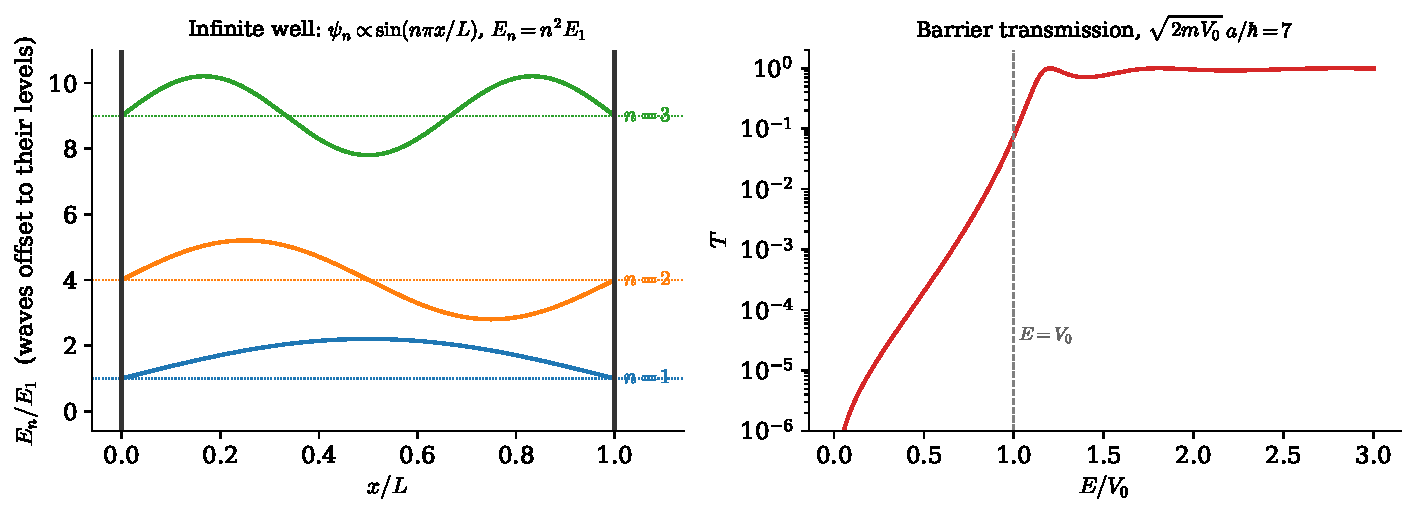
\includegraphics[width=0.97\textwidth]{fig_well_tunnel.pdf}
  \caption{One dimension, both regimes, exact formulas. \emph{Left}:
  the infinite well's first three stationary states
  \eqref{eq:box-spectrum}, each drawn at its energy --- the pinned
  string's mode shapes, now carrying quantum energies
  ($E_n \propto n^2$).
  \emph{Right}: barrier transmission \eqref{eq:transmission} (log
  scale) for $z_0 = \sqrt{2mV_0}\,a/\hbar = 7$: exponential
  tunneling below $V_0$, unit-transmission resonances above ---
  fitting waves again.}
  \label{fig:well-tunnel}
\end{figure}

\begin{example}[The scanning tunneling microscope]
\label{ex:stm}
The exponential in \eqref{eq:transmission} is an instrument. Between
an STM tip and a metal surface, the vacuum gap is a barrier of
height set by the work function, $\phi \approx 4.5\,\mathrm{eV}$
for typical metals, so
\begin{equation}
  \kappa = \frac{\sqrt{2 m_e \phi}}{\hbar}
  \approx 1.09\;\text{\AA}^{-1},
  \qquad
  \frac{T(a)}{T(a + 1\,\text{\AA})}
  = \ee^{2\kappa\cdot 1\,\text{\AA}}
  \approx 9 :
\end{equation}
the tunneling current changes by nearly an \emph{order of magnitude
per \aa ngstr\"om} of tip height. That extreme sensitivity is the
whole instrument: a feedback loop holding the current constant
traces the surface to sub-atomic precision, and every STM image of
individual atoms is Eq.~\eqref{eq:transmission}'s exponential read
out as topography.
\end{example}

\begin{remark}[Slow potentials: WKB in brief]
\label{rem:wkb}
Between the exactly solvable and the numerical lies the
\emph{slowly-varying} potential, and the ansatz that owns it is
worth one display even unproved:
\begin{equation}
  u(x) \;\approx\;
  \frac{C}{\sqrt{p(x)}}\;
  \exp\Bigl[\pm\frac{\ii}{\hbar}\int^x p(x')\,\dd x'\Bigr],
  \qquad
  p(x) = \sqrt{2m\bigl(E - V(x)\bigr)}
  \label{eq:wkb}
\end{equation}
--- the phase is the \emph{classical action} accumulating along the
path, the amplitude $p^{-1/2}$ is flux conservation
(\eqref{eq:continuity-qm}: constant $j = \rho\,p/m$ forces
$\rho \propto 1/p$), and the patching across turning points (where
$p \to 0$ and the ansatz fails; the exact linear-potential solution,
an Airy function, supplies the splice [stated; Hall Ch.\ 15]) yields the
Bohr--Sommerfeld quantization $\oint p\,\dd x = (n + \tfrac12)\,h$
of the old quantum theory [stated; Hall Ch.\ 15 gives the full
treatment].
Why the action sits in the phase is not explicable at this level ---
but it is two sections ahead: \S\ref{sec:path-integral} will show
every amplitude is a sum of $\ee^{\ii S/\hbar}$ over paths, and
\eqref{eq:wkb} is what that sum looks like when one path dominates.
The remark is a promise; \S\ref{sec:path-integral} keeps
it.
\end{remark}


%=======================================================================
\section{Quantizing the Harmonic Oscillator}
%=======================================================================
\label{sec:sho-quantum}

The object that opened the series --- one mass, one spring
[Osc.\ \S2] --- makes its fifth appearance, and its most
consequential: quantized here, it becomes in the outlook the atom
of every quantum field. The solution method is pure algebra --- no
differential equation is solved until the wavefunctions are wanted
--- and the algebraic engine, a ladder built from the commutator,
will be reused, unchanged, for angular momentum in
\S\ref{sec:J-spectrum}.

\subsection{Factorizing the Hamiltonian}
\label{sec:factorizing}

The Hamiltonian
\begin{equation}
  \op H = \frac{\op p^2}{2m} + \frac12\,m\omega^2\op q^2
\end{equation}
calls for factoring as a sum of squares,
$u^2 + v^2 = (u - \ii v)(u + \ii v)$ --- and the obstruction to
doing so, $[\op q, \op p] \ne 0$, turns out to carry all of the
problem's quantum content, as the derivation below makes explicit. Define the dimensionless combination (and its adjoint)
\begin{equation}
  \op a
  = \sqrt{\frac{m\omega}{2\hbar}}
    \Bigl(\op q + \frac{\ii\,\op p}{m\omega}\Bigr),
  \qquad
  \op a^\dagger
  = \sqrt{\frac{m\omega}{2\hbar}}
    \Bigl(\op q - \frac{\ii\,\op p}{m\omega}\Bigr),
  \label{eq:ladder-def}
\end{equation}
and multiply out, letting the cross terms manufacture the
commutator:
\begin{equation}
  \op a^\dagger\op a
  = \frac{m\omega}{2\hbar}
    \Bigl(
      \op q^2 + \frac{\op p^2}{m^2\omega^2}
    \Bigr)
  + \frac{\ii}{2\hbar}\,[\op q, \op p]
  = \frac{\op H}{\hbar\omega} - \frac12 ,
  \qquad
  [\op a, \op a^\dagger] = 1
\end{equation}
(the second relation by the same two lines with the sign flipped).
Hence
\begin{equation}
  \boxed{\;
  \op H = \hbar\omega\,\Bigl(\op N + \tfrac12\Bigr),
  \qquad
  \op N \equiv \op a^\dagger \op a,
  \qquad
  [\op a, \op a^\dagger] = 1 .
  \;}
  \label{eq:H-ladder}
\end{equation}

\begin{remark}[The classical amplitude promoted to an operator]
\label{rem:classical-amplitude}
Equation \eqref{eq:ladder-def} is not a clever guess; it is the
series' oldest move. From the classical oscillator's
amplitude--phase solution $q = A\cos(\omega t - \phi)$
[Osc.\ \S2.3], form the combination $z \equiv q + \ii p/m\omega
= q + \ii\dot q/\omega$: one line gives
$z = A\,\ee^{-\ii(\omega t - \phi)}$ [verified here] --- a complex
amplitude that rotates rigidly, $z(t) = z(0)\,\ee^{-\ii\omega t}$.
The operator $\op a$ \emph{is} the promotion of that combination
--- and the Heisenberg flow confirms it inherits the
rigid rotation:
$\dd\op a_H/\dd t = [\op a_H, \op H]/\ii\hbar
= -\ii\omega\,\op a_H$, so
$\op a_H(t) = \op a\,\ee^{-\ii\omega t}$, verbatim the classical
solution with a hat.
\end{remark}

\subsection{The spectrum from the algebra alone}
\label{sec:sho-spectrum}

Everything now follows from \eqref{eq:H-ladder} --- three steps, no
analysis.

\emph{Step 1: the ladder.} From
$[\op N, \op a] = [\op a^\dagger\op a, \op a]
= [\op a^\dagger, \op a]\,\op a = -\,\op a$ (Leibniz,
\eqref{eq:commutator-leibniz}), and its adjoint
$[\op N, \op a^\dagger] = +\,\op a^\dagger$: if
$\op N\ket\nu = \nu\ket\nu$, then
\begin{equation}
  \op N\,\bigl(\op a\ket\nu\bigr)
  = (\nu - 1)\,\bigl(\op a\ket\nu\bigr),
  \qquad
  \op N\,\bigl(\op a^\dagger\ket\nu\bigr)
  = (\nu + 1)\,\bigl(\op a^\dagger\ket\nu\bigr) :
\end{equation}
$\op a$ steps down the spectrum by one, $\op a^\dagger$ up.

\emph{Step 2: the floor.} Norms bound the ladder:
\begin{equation}
  \bigl\|\op a\ket\nu\bigr\|^2
  = \bra\nu\op a^\dagger\op a\ket\nu
  = \nu
  \;\ge\; 0 .
  \label{eq:ladder-bound}
\end{equation}
Descending from any $\nu$ produces eigenvalues $\nu - 1, \nu - 2,
\dots$, which \eqref{eq:ladder-bound} forbids from passing below
zero --- so the descent must \emph{terminate}: some rung is
annihilated, $\op a\ket{\nu_{\min}} = 0$, and then
\eqref{eq:ladder-bound} says $\nu_{\min} = 0$. Termination is only
possible if the starting $\nu$ was a whole number of steps above
zero:
\begin{equation}
  \nu = n \in \{0, 1, 2, \dots\} .
\end{equation}

\emph{Step 3: the bookkeeping.} Fixing phases,
\begin{equation}
  \boxed{\;
  E_n = \hbar\omega\Bigl(n + \tfrac12\Bigr),
  \qquad
  \op a\ket n = \sqrt n\,\ket{n{-}1},
  \qquad
  \op a^\dagger\ket n = \sqrt{n{+}1}\,\ket{n{+}1},
  \qquad
  \ket n = \frac{(\op a^\dagger)^n}{\sqrt{n!}}\,\ket 0 .
  \;}
  \label{eq:sho-spectrum}
\end{equation}
The spectrum \S\ref{sec:classical-failures} demanded --- energy in
uniform lumps of $\hbar\omega$ --- is now a theorem: the ladder has
constant rungs because $[\op a, \op a^\dagger]$ is a \emph{number}.
[Completeness of the $\ket n$ --- that the ladder built from
$\ket 0$ exhausts the Hilbert space --- is true and quietly
nontrivial; Hall \S11.4. Stated.]

\begin{remark}[The floor is the Gaussian again]
\label{rem:sho-ground-gaussian}
The termination condition $\op a\ket 0 = 0$ is, written out via
\eqref{eq:ladder-def},
$(\op p - \ii\, m\omega\,\op q)\ket 0 = 0$ --- which is
\emph{verbatim} the minimum-uncertainty condition
\eqref{eq:min-uncertainty-condition} with $\lambda = m\omega$ and
centers at the origin. The oscillator's ground state \emph{is} the
Gaussian of \S\ref{sec:gaussian-packet}, width
$(\Delta q)^2 = \hbar/2m\omega$, sitting exactly on the floor
$\Delta q\,\Delta p = \hbar/2$; and the zero-point energy is that
floor expressed as an energy --- minimizing
$\langle H\rangle = (\Delta p)^2/2m + \tfrac12 m\omega^2(\Delta q)^2$
subject to the uncertainty bound gives exactly $\hbar\omega/2$, the
algebra's $\tfrac12$ re-derived as a variational fact. The particle
cannot sit at the bottom of the well for the same reason the atom of
Example~\ref{ex:atomic-size} cannot collapse: stillness is
not an available state.
\end{remark}

\begin{example}[One molecule's quantum and frozen heat]
\label{ex:CO}
Carbon monoxide's vibrational frequency, spectroscopically
$\tilde\nu = 2143\,\mathrm{cm}^{-1}$, puts its quantum at
\begin{equation}
  \hbar\omega = hc\tilde\nu
  \approx 4.26\times10^{-20}\,\mathrm J
  \approx 0.266\,\mathrm{eV},
  \qquad
  \frac{\hbar\omega}{k_B T}\bigg|_{300\,\mathrm K}
  \approx 10.3 :
\end{equation}
ten times the thermal energy, so the Boltzmann weight of even the
first excited rung is $\ee^{-10.3} \approx 3\times10^{-5}$ --- at
room temperature the vibration is \emph{frozen out}, the molecule
locked to $n = 0$, and the vibrational degree of freedom silently
withdraws from the specific heat. Classical equipartition's
room-temperature failure --- half of
\S\ref{sec:classical-failures}'s second bullet --- is this number;
the first rung sits an order of magnitude above the thermal
energy.
\end{example}

\subsection{Wavefunctions from the ladder}
\label{sec:sho-wavefunctions}

When shapes are wanted, the algebra dictates them. The ground state
solves $\op a\, u_0 = 0$ in the position representation --- a
first-order equation,
$(m\omega x + \hbar\,\partial_x)\,u_0 = 0$, whose solution is the
Gaussian Remark~\ref{rem:sho-ground-gaussian} promised --- and every
excited state is $(\op a^\dagger)^n$ applied to it: each application
of $\op a^\dagger \propto (m\omega x - \hbar\partial_x)$ multiplies
by a polynomial of one higher degree, generating the Hermite family,
\begin{equation}
  u_n(x)
  = \Bigl(\frac{m\omega}{\pi\hbar}\Bigr)^{1/4}
    \frac{1}{\sqrt{2^n n!}}\;
    H_n(\xi)\;\ee^{-\xi^2/2},
  \qquad
  \xi = x\,\sqrt{\frac{m\omega}{\hbar}}
  \label{eq:hermite}
\end{equation}
[normalizations stated; the generation from $\op a^\dagger$ is the
proof strategy, and it also delivers $n$ nodes for $u_n$ --- the
oscillation theorem of \S\ref{sec:box} passing its check].
Figure~\ref{fig:sho} shows the family at its rungs, tails
penetrating the classically forbidden region --- tunneling's
kinship (\S\ref{sec:tunneling}) --- and, at $n = 20$, the
correspondence principle in the flesh: the quantum density's ripples
average to the classical dwell-time distribution
$1/\pi\sqrt{A^2 - x^2}$, largest at the turning points where the
classical particle lingers.

\begin{figure}[htbp]
  \centering
  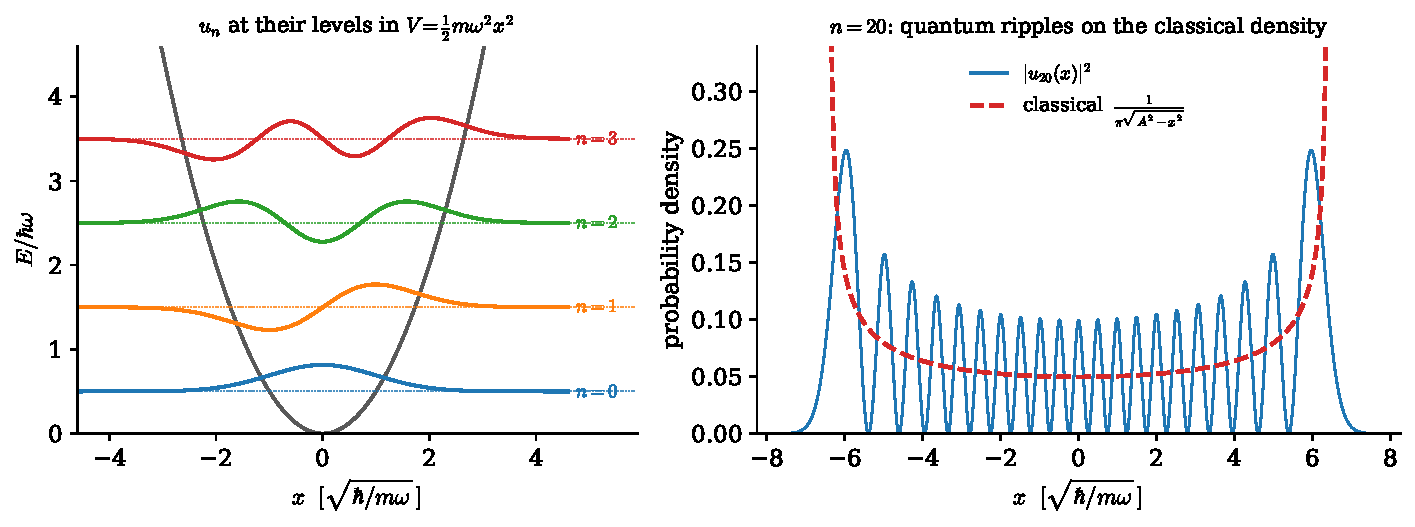
\includegraphics[width=0.97\textwidth]{fig_sho.pdf}
  \caption{The quantized oscillator, exact formulas
  ($\hbar = m = \omega = 1$). \emph{Left}: eigenfunctions
  \eqref{eq:hermite}, $n = 0$--$3$, at their levels
  $E_n = n + \tfrac12$ in the potential --- equal rungs, $n$ nodes,
  Gaussian floor, forbidden-region tails. \emph{Right}: at $n = 20$
  the quantum density ripples about the classical dwell-time
  distribution (dashed), which diverges at the turning points
  $\pm A$, $A = \sqrt{2E_n}$ --- the correspondence principle,
  drawn.}
  \label{fig:sho}
\end{figure}

\subsection{Coherent states: where the classical oscillator lives}
\label{sec:coherent}

Ehrenfest (\S\ref{sec:ehrenfest}) promised that quadratic potentials
evolve packet centers exactly classically; here are the packets that
take fullest advantage. Define \emph{coherent states} as eigenstates
of the (non-Hermitian --- eigenkets are still legal) lowering
operator,
\begin{equation}
  \op a\,\ket\alpha = \alpha\,\ket\alpha,
  \qquad \alpha \in \C,
  \qquad
  \ket\alpha
  = \ee^{-|\alpha|^2/2}
    \sum_{n=0}^{\infty}
    \frac{\alpha^n}{\sqrt{n!}}\,\ket n
  \label{eq:coherent}
\end{equation}
(the expansion follows by feeding $\sum c_n\ket n$ to the
eigenvalue equation, whence
$c_{n} = \alpha\,c_{n-1}/\sqrt n$ by \eqref{eq:sho-spectrum}). Three properties make them the classical
limit's residents:
\begin{itemize}
  \item \textbf{They stay coherent, and $\alpha$ rotates
  classically.} Apply \eqref{eq:phase-evolution} to
  \eqref{eq:coherent}: the phases $\ee^{-\ii E_n t/\hbar}$
  reassemble the same sum with
  $\alpha \to \alpha\,\ee^{-\ii\omega t}$ (times a global phase) ---
  the label traces exactly the classical complex amplitude of
  Remark~\ref{rem:classical-amplitude}, so
  $\langle q\rangle(t)$ and $\langle p\rangle(t)$ run the classical
  trajectory \emph{exactly}, at any amplitude.
  \item \textbf{They ride the floor.} A coherent state is the ground
  -state Gaussian rigidly displaced (in $q$ and $p$ by
  $\operatorname{Re}$, $\operatorname{Im}$ of $\alpha$), so it
  saturates $\Delta q\,\Delta p = \hbar/2$ at every instant [one-line
  check: $\op a\ket\alpha = \alpha\ket\alpha$ \emph{is} the
  minimum-uncertainty condition with shifted centers] --- a
  wave packet that oscillates forever \emph{without spreading}, the
  loophole to \S\ref{sec:spreading} that only the quadratic
  potential's rigidity permits.
  \item \textbf{They are what ``classical amplitude $A$'' means.}
  The excitation statistics are Poisson,
  $P(n) = \ee^{-|\alpha|^2}|\alpha|^{2n}/n!$, with mean
  $\langle N\rangle = |\alpha|^2$: a macroscopic oscillation is a
  coherent state with $|\alpha|^2 \sim S_{\text{cl}}/\hbar \gg 1$
  quanta --- the $S/\hbar$ switch of
  \S\ref{sec:brackets-commutators} counting rungs --- and laser
  light is, to excellent approximation, this state of the
  electromagnetic field's modes. [stated; quantum optics'
  founding fact.]
\end{itemize}

\medskip
\noindent
One bookkeeping note closes the section, aimed at the outlook: the
pair $(\op a, \op a^\dagger)$ with $[\op a, \op a^\dagger] = 1$ is
the entire quantum content of \emph{one} oscillator --- and
[Fld.\ \S14.1] showed a free field is a countable family of them,
one per wavevector. Quantizing the field will mean writing one
ladder per mode, $[\op a_{\vec k}, \op a^\dagger_{\vec k'}] =
\delta_{\vec k\vec k'}$, and reading $\op a^\dagger_{\vec k}\ket 0$
as \emph{a particle}. Every technical prerequisite for that sentence
is now on the table.


%=======================================================================
\section{The Propagator by Two Routes}
%=======================================================================
\label{sec:path-integral}

The field-theory notes could only \emph{mark} the fork between the
two quantizations --- canonical, with its time slicing, and the path
integral, built on the scalar action [Fld.\ \S10.3]. This section
walks both roads in full, at the one level where both are completely
tractable, and verifies they arrive at the same place. Along the
way it keeps the promise of Remark~\ref{rem:wkb}, answers the
series' oldest open question --- \emph{why} nature extremizes
actions --- and returns the central object of the mechanics notes,
the action, as a phase.

\subsection{The object: the propagator and its composition law}
\label{sec:propagator-def}

Define the \emph{propagator} as the open sandwich of
\S\ref{sec:computational-moves}(d) with the evolution inside:
\begin{equation}
  \boxed{\;
  K(x_b, T;\, x_a, 0)
  \;\equiv\;
  \bra{x_b}\,U(T)\,\ket{x_a}
  \;}
  \label{eq:propagator-def}
\end{equation}
--- the amplitude to be found at $x_b$ after time $T$, having
started at $x_a$. It carries the whole of dynamics: inserting
$\idop = \int\dd x_a\ket{x_a}\bra{x_a}$ into
$\ket{\psi(T)} = U(T)\ket{\psi(0)}$,
\begin{equation}
  \psi(x_b, T)
  = \int\dd x_a\;
    K(x_b, T; x_a, 0)\;\psi(x_a, 0),
\end{equation}
so solving for $K$ solves every initial-value problem at once. And
it obeys one structural identity, obtained by splitting
$U(T) = U(T - t_c)\,U(t_c)$ and inserting a position resolution
between the factors:
\begin{equation}
  K(x_b, T; x_a, 0)
  = \int\dd x_c\;
    K(x_b, T; x_c, t_c)\;
    K(x_c, t_c; x_a, 0) :
  \label{eq:composition}
\end{equation}
\emph{amplitudes for successive legs multiply; amplitudes for
alternative waypoints add.} Equation \eqref{eq:composition} looks
like bookkeeping. Iterated, it is a theory
(\S\ref{sec:time-slicing}).

\subsection{Route 1: the spectral representation}
\label{sec:spectral-route}

Canonically, $K$ is computed by diagonalizing: insert the energy
eigenbasis into \eqref{eq:propagator-def},
\begin{equation}
  K(x_b, T; x_a, 0)
  = \sum_n
    u_n(x_b)\,u_n^{*}(x_a)\;
    \ee^{-\ii E_n T/\hbar}
  \label{eq:spectral-rep}
\end{equation}
--- the whole kernel, from the spectrum. For the free particle the
sum is an integral over momentum eigenstates
\eqref{eq:momentum-eigenstate}, and it is a Gaussian
(Appendix~\ref{app:gaussians}, in its Fresnel form
\eqref{eq:fresnel}):
\begin{align}
  K_{\text{free}}
  &= \int\frac{\dd p}{2\pi\hbar}\;
    \exp\Bigl[
      \frac{\ii}{\hbar}\Bigl(
        p\,(x_b - x_a) - \frac{p^2 T}{2m}
      \Bigr)
    \Bigr]
  \notag\\[2pt]
  &= \sqrt{\frac{m}{2\pi\ii\hbar\, T}}\;
    \exp\Bigl[
      \frac{\ii}{\hbar}\,
      \frac{m\,(x_b - x_a)^2}{2T}
    \Bigr]
  \label{eq:free-propagator}
\end{align}
(complete the square in $p$; the shifted Gaussian is
\eqref{eq:gaussian-linear}--\eqref{eq:fresnel}). Now look hard at
the exponent. The quantity $m(x_b - x_a)^2/2T$ is
$\tfrac12 m v^2\, T$ for the uniform motion connecting the
endpoints --- it is \emph{the classical action of the classical
path},
\begin{equation}
  K_{\text{free}}
  = \sqrt{\frac{m}{2\pi\ii\hbar\, T}}\;
    \ee^{\,\ii S_{\text{cl}}/\hbar} .
  \label{eq:free-Scl}
\end{equation}
Nothing in Route 1 asked for the action; no Lagrangian was
mentioned; and yet the action of [Mech.] stands in the exponent.
Route 1 cannot explain this. Route 2 is the
explanation.

\subsection{Route 2: time slicing and the sum over paths}
\label{sec:time-slicing}

Iterate the composition law \eqref{eq:composition} $N - 1$ times
with uniform slices $\varepsilon = T/N$:
\begin{equation}
  K(x_b, T; x_a, 0)
  = \int \dd x_1 \cdots \dd x_{N-1}\;
    \prod_{j=0}^{N-1}
    \bra{x_{j+1}}\,U(\varepsilon)\,\ket{x_j},
  \qquad x_0 = x_a,\ x_N = x_b .
\end{equation}
Only the \emph{short-time} amplitude is needed, and for
$\op H = \op p^2/2m + V(\op q)$ the two terms can be exponentiated
separately at cost $O(\varepsilon^2)$ per slice [stated; the Trotter
product formula is the precise justification]. The kinetic factor is
computed by inserting momentum states --- the identical Gaussian as
\eqref{eq:free-propagator} with $T \to \varepsilon$ --- and the
potential factor is diagonal:
\begin{equation}
  \bra{x_{j+1}} U(\varepsilon)\ket{x_j}
  \approx
  \sqrt{\frac{m}{2\pi\ii\hbar\varepsilon}}\;
  \exp\Biggl[
    \frac{\ii\varepsilon}{\hbar}
    \biggl(
      \frac m2
      \Bigl(\frac{x_{j+1} - x_j}{\varepsilon}\Bigr)^{\!2}
      - V(x_j)
    \biggr)
  \Biggr].
\end{equation}
Multiply the slices: the exponents \emph{add}, and what they add up
to is a Riemann sum ---
\begin{equation}
  \sum_{j}\varepsilon
  \Bigl[
    \frac m2\Bigl(\frac{\Delta x_j}{\varepsilon}\Bigr)^2
    - V(x_j)
  \Bigr]
  \;\xrightarrow[N \to \infty]{}\;
  \int_0^T \dd t\;
  \Bigl[\frac m2\,\dot x^2 - V(x)\Bigr]
  \;=\; S[x] ,
\end{equation}
the \emph{action} of [Mech.\ \S3], kinetic minus potential,
evaluated along the broken-line path through the waypoints. In the
limit:
\begin{equation}
  \boxed{\;
  K(x_b, T; x_a, 0)
  \;=\;
  \int\!\mathcal D x(t)\;\;
  \ee^{\,\ii S[x]/\hbar}
  \;}
  \label{eq:path-integral}
\end{equation}
--- the \emph{path integral}, with $\mathcal Dx$ shorthand for the
sliced measure and its prefactors [the continuum measure's
existence is a genuine mathematical subtlety; stated, with the
sliced definition as the operational meaning]. The reading
(Fig.~\ref{fig:paths}): \emph{every} path from $(x_a, 0)$ to
$(x_b, T)$ contributes --- jagged, backtracking, absurd ones
included --- all with the \emph{same magnitude}, distinguished only
by a phase, and the phase is the classical action in units of
$\hbar$. Democracy of paths; the classical trajectory holds no
privilege in the integrand.

\begin{figure}[htbp]
  \centering
  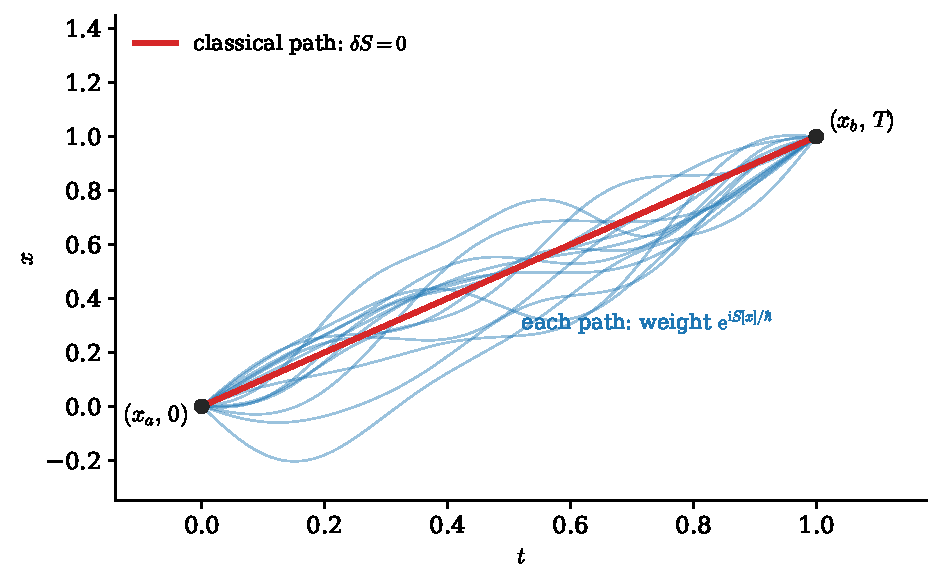
\includegraphics[width=0.62\textwidth]{fig_paths.pdf}
  \caption{The sum over paths \eqref{eq:path-integral}: every
  history from $(x_a, 0)$ to $(x_b, T)$ carries the same weight in
  magnitude, phase $S[x]/\hbar$. The classical path (bold) is
  distinguished not by the integrand but by \emph{interference}:
  it is where the phase is stationary, so neighboring paths add
  coherently instead of canceling.}
  \label{fig:paths}
\end{figure}

\subsection{Stationary phase: the origin of Hamilton's principle}
\label{sec:stationary-phase}

Where does the classical world sit inside
\eqref{eq:path-integral}? In the interference. When
$S \gg \hbar$ --- the switch of \S\ref{sec:brackets-commutators},
one last time --- the phase $S[x]/\hbar$ spins wildly under any
deformation of the path, and contributions cancel in pairs \emph{%
except} where the phase is stationary:
\begin{equation}
  \delta S[x] = 0
  \qquad\text{--- Hamilton's principle.}
\end{equation}
The variational principle that the mechanics notes installed as
their axiom [Mech.\ \S3] is hereby demoted and thereby explained:
\emph{it is the stationary-phase approximation to the sum over
histories} --- nature does not prefer the extremal path; it takes
all of them, and only near the extremum do the amplitudes survive
their own interference. This answers the question the mechanics
notes could only postpone --- why extremizing $S$ was ever the
right principle --- and it keeps
Remark~\ref{rem:wkb}'s promise: the WKB
wavefunction \eqref{eq:wkb}, action in the phase and flux in the
amplitude, is exactly what \eqref{eq:path-integral} looks like when
one stationary path dominates and Gaussian fluctuations around it
supply the prefactor.

For \emph{quadratic} Lagrangians the story sharpens from
approximation to identity: expanding
$x(t) = x_{\text{cl}}(t) + \eta(t)$, the action splits exactly ---
$S[x] = S_{\text{cl}} + S_2[\eta]$ with no higher terms, the linear
term absent by $\delta S = 0$ --- and the fluctuation integral
factors off as an endpoint-independent function of time:
\begin{equation}
  K = F(T)\;\ee^{\,\ii S_{\text{cl}}/\hbar}
  \qquad\text{(exactly, for quadratic } L\text{)} .
  \label{eq:quadratic-exact}
\end{equation}
That is why \eqref{eq:free-Scl}'s exponent was \emph{exactly} the
classical action: the free particle is quadratic. So is the
oscillator --- the payoff:

\paragraph{Route 2 applied to the oscillator, with Route 1 as the check.} The
classical action of the harmonic path between fixed endpoints is a
classical-mechanics exercise in [Mech.]'s toolkit:
\begin{equation}
  S_{\text{cl}}
  = \frac{m\omega}{2\sin\omega T}
    \Bigl[
      (x_a^2 + x_b^2)\cos\omega T - 2\,x_a x_b
    \Bigr],
\end{equation}
and the fluctuation factor [computable as a product over the modes
of $S_2$; stated --- or fixed, more cheaply, by matching the
$\omega \to 0$ free limit \eqref{eq:free-propagator}] completes the
kernel:
\begin{equation}
  K_{\text{SHO}}
  = \sqrt{\frac{m\omega}{2\pi\ii\hbar\,\sin\omega T}}\;
    \exp\Bigl[\frac{\ii}{\hbar}\,S_{\text{cl}}\Bigr].
  \label{eq:mehler}
\end{equation}
Route 1 now checks Route 2. Set $x_a = x_b = x$ and integrate ---
the \emph{trace} of the propagator, which by the spectral
representation \eqref{eq:spectral-rep} must equal
$\sum_n \ee^{-\ii E_n T/\hbar}$. The integral is one more Gaussian
(exponent
$\ii m\omega\,x^2(\cos\omega T - 1)/\hbar\sin\omega T$, Appendix
\ref{app:gaussians}), and with $1 - \cos\omega T =
2\sin^2(\omega T/2)$:
\begin{equation}
  \int\dd x\; K_{\text{SHO}}(x, T; x, 0)
  = \frac{1}{2\ii\,\sin(\omega T/2)}
  = \frac{\ee^{-\ii\omega T/2}}{1 - \ee^{-\ii\omega T}}
  = \sum_{n=0}^{\infty}
    \ee^{-\ii\omega\left(n + \frac12\right) T}
  \label{eq:trace-check}
\end{equation}
[the geometric series converges under the standard
$T \to T(1 - \ii\epsilon)$ prescription; stated]
--- a geometric series whose exponents read off
$E_n = \hbar\omega(n + \tfrac12)$: \emph{the path integral knows the
ladder's spectrum} \eqref{eq:sho-spectrum}, rung for rung, zero-%
point included. Two routes, one kernel, one spectrum; the fork's two
roads, walked to the same destination and checked against each
other.

\begin{remark}[The fork revisited]
\label{rem:fork-revisited}
[Fld.\ \S10.3] could only gesture at what has just been done in
full. The canonical route (Routes 1 here, Heisenberg/Schr\"odinger
machinery throughout) slices time: unitarity is manifest, but a
frame has been chosen --- the same trade-off, at the same Legendre
step, as in the mechanics and field notes. The path-integral route weights
histories by the \emph{scalar} $S[x]$: no slicing in the weight, no
picture, no operator ordering --- but unitarity is now a theorem to
prove rather than a structure to see. At this document's level the
choice is convenience; one level up, where $S$ is the Lorentz
scalar of [Fld.\ \S8.1], the path integral is what keeps covariance
visible while the canonical formalism keeps probability visible ---
and quantum field theory, needing both, keeps both formalisms and
translates freely. The translation's proof of concept is this
section: \eqref{eq:spectral-rep} and \eqref{eq:path-integral} are
the same object, as \eqref{eq:trace-check} verifies.
\end{remark}

\medskip
\noindent
Part II is complete: evolution, pictures, spectra, and the two
grand formalisms reconciled on the series' own mascot. Part III
turns from time to \emph{space} --- rotations, and everything the
word ``angular momentum'' is about to mean.


%=======================================================================
\clearpage
\part{Symmetry}
%=======================================================================

%=======================================================================
\section{Rotations and Angular Momentum}
%=======================================================================
\label{sec:rotations}

Part III is the symmetry part, and it opens by finishing a table.
The quantum Noether dictionary
(Remark~\ref{rem:quantum-noether}) has run twice --- translations
yielded $\op p$, waiting yielded $\op H$ --- and its third row,
rotations, is richer than both: three generators instead of one,
and, for the first time, generators that \emph{do not commute with
each other}. That non-commutativity is inherited straight from the
geometry of turning, it reproduces the classical bracket algebra of
the mechanics notes on cue, and it is loose enough ---
no $\idop$ on its right-hand side --- to admit the finite-%
dimensional representations that Theorem~\ref{thm:no-finite-dim}
exempted. The standing laboratory is about to receive its
derivation.

\subsection{Symmetries act unitarily}
\label{sec:wigner-theorem}

What should ``the system, rotated'' mean on Hilbert space? A map
$\ket\alpha \to \ket{\alpha'}$ that preserves all physical
predictions --- all transition probabilities,
$|\braket\beta\alpha|^2$. A foundational theorem pins down what
such maps can be:

\begin{theorem}[Wigner]\label{thm:wigner}
Any map of rays preserving all transition probabilities is
implemented by an operator that is either unitary or antiunitary.
[stated; the antiunitary option is realized in nature by time
reversal, and is deferred with it.]
\end{theorem}

\noindent
Continuous symmetries connect to the identity, which is unitary, so
each rotation $R$ acts by a unitary $U(R)$, and composition respects
the group --- up to a phase, since states are rays
(\S\ref{sec:kets}): $U(R_2)U(R_1) = \ee^{\ii\gamma}\,
U(R_2 R_1)$. That innocent-looking phase has consequences: for most
groups it can be removed by redefinitions; for the rotation group
the irreducible ambiguity is exactly a \emph{sign} --- the sign
Remark~\ref{rem:2pi-seed} watched a precessing spin acquire --- and
\S\ref{sec:su2} is where it surfaces. [stated at this level;
the classification of the phases is the theory of projective
representations.]

For an infinitesimal rotation by $\dd\varphi$ about the axis
$\hat n$, the third run of the generator move
(\S\ref{sec:translation}, \S\ref{sec:evolution-operator}):
\begin{equation}
  U(\hat n, \dd\varphi)
  = \idop
  - \frac{\ii}{\hbar}\,\dd\varphi\;
    \hat n\cdot\op{\vec J}
  + O(\dd\varphi^2),
  \label{eq:J-generator}
\end{equation}
defining three Hermitian generators $\op J_x, \op J_y, \op J_z$ ---
the \emph{angular momentum} operators, $[\op J] = [\text{action}]$
this time, no $\hbar$-repair needed --- and completing the
dictionary's table. What remains is their algebra.

\subsection{The algebra by both roads}
\label{sec:rotation-algebra}

The document's standing pattern --- one commutator, two independent
derivations --- applies verbatim.

\emph{Road A: deform the classical bracket.} The mechanics notes
recorded the closed bracket of the classical angular momenta,
$\{L_x, L_y\} = L_z$ [Mech.\ \S8.2]; the full family
$\{L_i, L_j\} = \epsilon_{ijk} L_k$ is the same two-line
computation from the fundamental brackets, run for each pair
[verify once]. Dirac's rule
\eqref{eq:dirac-rule} transcribes in one line:
\begin{equation}
  \boxed{\;
  [\op J_i, \op J_j]
  = \ii\hbar\,\epsilon_{ijk}\,\op J_k .
  \;}
  \label{eq:J-algebra}
\end{equation}

\emph{Road B: read the geometry of turning.} Rotations about
different axes do not commute, and the failure is quantitative.
For the $3\times3$ rotation matrices, a direct expansion to second
order gives the classic identity
\begin{equation}
  R_x(\varepsilon)\,R_y(\varepsilon)\,
  R_x(-\varepsilon)\,R_y(-\varepsilon)
  = R_z(\varepsilon^2) + O(\varepsilon^3)
  \label{eq:rotation-commutator}
\end{equation}
--- go around the little $x$--$y$ commutator loop and you have
turned, slightly, about $z$ (verify once with the matrices: the
$O(\varepsilon)$ terms cancel by construction, and the surviving
$\varepsilon^2$ entries sit exactly in the $xy$ block). Demand that
the unitaries represent this, insert \eqref{eq:J-generator} on both
sides, and match at order $\varepsilon^2$: the left side's surviving
second-order term is
$-[\op J_x, \op J_y]\,\varepsilon^2/\hbar^2$ (the $\op J_x^2$ and
$\op J_y^2$ terms cancel pairwise between the $+\varepsilon$ and
$-\varepsilon$ factors), the right side's is
$-\ii\op J_z\,\varepsilon^2/\hbar$, whence
$[\op J_x, \op J_y] = \ii\hbar\,\op J_z$ --- \eqref{eq:J-algebra}
again, cyclically. The two roads' agreement is
Remark~\ref{rem:quantum-noether}'s convergence, third instance: the
bracket algebra of mechanics \emph{was} the geometry of the
symmetry group all along, and quantization preserves both because
they are one.

\begin{remark}[Why the laboratory was allowed]
\label{rem:finite-dim-legal}
Look at the right-hand side of \eqref{eq:J-algebra}: operators, not
$\ii\hbar\,\idop$. The trace obstruction of
Theorem~\ref{thm:no-finite-dim} evaporates ---
$\operatorname{tr}\,\epsilon_{ijk}\op J_k = 0$ is perfectly
satisfiable by traceless matrices --- and finite-dimensional
representations are \emph{allowed}: the algebra itself does not fix
the size of its stage, and \S\ref{sec:J-spectrum} will find one
stage per half-integer. The two-dimensional laboratory of
\S\ref{sec:spin-half} has operated on exactly this exemption since
\S\ref{sec:algebra-consequences} first noted it; the exemption is
now explained.
\end{remark}

\subsection{Orbital angular momentum: the classical entry}
\label{sec:orbital}

The oldest realization of \eqref{eq:J-algebra} is the quantized
classical angular momentum,
\begin{equation}
  \op L_i = \epsilon_{ijk}\,\op q_j\,\op p_k
\end{equation}
(no ordering ambiguity: $\epsilon_{ijk}$ only pairs $j \ne k$, and
$[\op q_j, \op p_k] = 0$ for $j \ne k$ --- Dirac's rule applies
without ambiguity). Verify the family with a single commutator:
\begin{align}
  [\op L_x, \op L_y]
  &= [\op q_y\op p_z - \op q_z\op p_y,\;
      \op q_z\op p_x - \op q_x\op p_z]
  \notag\\
  &= \op q_y\op p_x\,[\op p_z, \op q_z]
   + \op q_x\op p_y\,[\op q_z, \op p_z]
  = \ii\hbar\,\bigl(\op q_x\op p_y - \op q_y\op p_x\bigr)
  = \ii\hbar\,\op L_z
\end{align}
(only the terms sharing a $z$-pair survive; Leibniz
\eqref{eq:commutator-leibniz} does the bookkeeping). And $\op L$
is a generator in the concrete sense: in polar coordinates on
the plane, the same two-line computation as
\S\ref{sec:p-position-rep} --- drag the wavefunction,
$\psi(\varphi - \dd\varphi)$, match against the generator --- gives
\begin{equation}
  \bra{\vx}\,\op L_z\,\ket\psi
  = -\,\ii\hbar\,\pd{}{\varphi}\,\psi(\vx) :
  \label{eq:Lz-polar}
\end{equation}
$\op L_z$ is to the angle what $\op p$ was to position --- with the
one crucial difference that the angle is \emph{periodic}, which is
about to quantize $\op L_z$'s spectrum (\S\ref{sec:J-spectrum}) by
the same fitting-waves mechanism as \S\ref{sec:box}, and which is
the constructive face of the bounded-coordinate warning in
Remark~\ref{rem:uncertainty-counterexample}.

\subsection{Spin: internal rotation and the sign}
\label{sec:spin-formalized}

Now the laboratory itself. Spin is angular momentum with no
$\op q\times\op p$ inside --- generators acting on an
\emph{internal} index of the state, touching the spatial argument
not at all: the precise analogue of the internal--spacetime split
that [Fld.\ \S9.3] drew for field symmetries. For spin-$\tfrac12$,
$\op S_i = \tfrac\hbar2\sigma_i$, and the Pauli identity
\eqref{eq:pauli-algebra}'s antisymmetric part \emph{is}
\eqref{eq:J-algebra} --- verified back in \S\ref{sec:spin-half},
now recognized as the rotation algebra in its smallest allowed
representation (Remark~\ref{rem:finite-dim-legal}).

The finite rotations come cheap, and they carry the section's
punchline. Exponentiate the generator using the Pauli identity's
symmetric part, $(\hat n\cdot\vec\sigma)^2 = \idop$: the power
series splits into even and odd,
\begin{equation}
  \boxed{\;
  U(\hat n, \varphi)
  = \exp\Bigl[
      -\frac{\ii\varphi}{2}\,\hat n\cdot\vec\sigma
    \Bigr]
  = \cos\frac\varphi2\;\idop
  \;-\; \ii\,\sin\frac\varphi2\;\hat n\cdot\vec\sigma ,
  \;}
  \label{eq:spin-rotation}
\end{equation}
--- and set $\varphi = 2\pi$:
\begin{equation}
  U(\hat n, 2\pi) = -\,\idop .
  \label{eq:minus-one}
\end{equation}
A full turn is \emph{minus} the identity --- for any axis, any
spin-$\tfrac12$ state. Remark~\ref{rem:2pi-seed} watched one
Hamiltonian produce this sign dynamically; \eqref{eq:minus-one}
says the Hamiltonian was innocent: the sign belongs to the
\emph{representation}, hard-wired into \eqref{eq:spin-rotation}'s
half-angles, which trace back through the exponential to the
$\tfrac\hbar2$ in the generators --- to what spin-$\tfrac12$
\emph{is}. It is also exactly the projective phase
Theorem~\ref{thm:wigner}'s fine print permitted: $U(2\pi)$
represents the same rotation as $U(0)$, differing by a sign that
rays cannot see but interferometers can. What kind of mathematical
object carries such a representation --- and what experiment
measures the sign --- is the next section entire.


%=======================================================================
\section{$SU(2)$, $SO(3)$, and the Double Cover}
%=======================================================================
\label{sec:su2}

Section~\ref{sec:spin-formalized} left a sign in the room:
$U(2\pi) = -\idop$, hard-wired into the half-angles of
\eqref{eq:spin-rotation}. This section identifies the sign's origin
--- the states of a spin-$\tfrac12$ do not carry the rotation group
at all, but its \emph{double cover} --- explains why no redefinition
can remove it, and then does what a physics document must: reports
the experiment in which the sign was measured, interference fringes
with a period of $720^\circ$.

\subsection{Two groups for one geometry}
\label{sec:two-groups}

The rotation group $SO(3)$ is an old acquaintance: the
$\mathsf G = \idop$, $\det = +1$ member of the one-template family
$\mathsf M^{\mathsf T}\mathsf G\,\mathsf M = \mathsf G$ [Fld.\
\S3.1] --- this subsection is that remark's quantum sequel. The new
group is the one \S\ref{sec:spin-formalized} was unknowingly
computing in: $SU(2)$, the $2\times2$ unitaries of unit
determinant. Its general element is exactly
\eqref{eq:spin-rotation},
\begin{equation}
  U = a\,\idop + \ii\,\vec b\cdot\vec\sigma,
  \qquad
  a, \vec b \in \R,
  \qquad
  a^2 + |\vec b|^2 = 1
  \label{eq:su2-param}
\end{equation}
(unitarity plus $\det U = 1$ force real $(a, \vec b)$ on the unit
sphere) --- so as a space, \emph{$SU(2)$ is the three-sphere}
$S^3$. The bridge to rotations is conjugation. Package a vector as
a matrix, $X = \vx\cdot\vec\sigma$, and let $U$ act by
\begin{equation}
  X \;\longrightarrow\; U\,X\,U^\dagger
  \;\equiv\; \vx'\cdot\vec\sigma .
  \label{eq:covering-map}
\end{equation}
The map $\vx \to \vx'$ is linear, and it is a \emph{rotation} by a
two-line argument: $\det X = -|\vx|^2$ (write it out from
\eqref{eq:pauli}), conjugation preserves determinants, so lengths
are preserved; and $SU(2)$ being connected, the map connects to the
identity --- orientation preserved, $R(U) \in SO(3)$. Composition
is automatic, $R(U_2 U_1) = R(U_2)R(U_1)$. But the correspondence
is not one-to-one:
\begin{equation}
  \boxed{\;
  R(-U) = R(U)
  \;}
  \qquad\text{--- two elements of } SU(2)
  \text{ per rotation,}
  \label{eq:two-to-one}
\end{equation}
since the sign cancels between $U$ and $U^\dagger$ in
\eqref{eq:covering-map} (and $\pm U$ are the \emph{only} such pairs:
the kernel is the center $\{\pm\idop\}$). $SU(2)$ is a
\emph{double cover} of $SO(3)$: the sphere $S^3$, wrapped twice
around the space of rotations, antipodal points $U, -U$ landing on
the same $R$. The spin-$\tfrac12$ sign is now identified rather
than mysterious: the state transforms under $SU(2)$; ``rotate by
$2\pi$'' is a path in $SO(3)$ that returns to the identity, but its
\emph{lift} to $SU(2)$ walks from $\idop$ to the other preimage,
$-\idop$ --- which re-derives Eq.~\eqref{eq:minus-one} as a
statement of geography.

\begin{remark}[Why the sign cannot be redefined away]
\label{rem:topology}
Could a cleverer assignment of phases make $U(2\pi) = +\idop$? No,
and the obstruction is topological. In $SO(3)$ the $2\pi$-rotation
loop \emph{cannot be continuously contracted to a point} --- the
group is not simply connected, $\pi_1(SO(3)) = \mathbb Z_2$
[stated; the ``belt trick'' is the tabletop proof, and the
$4\pi$ loop \emph{does} contract] --- so a representation is free
to assign the loop a sign, and no continuous redefinition can
change a discrete assignment. $SU(2) = S^3$ \emph{is} simply
connected: it is the universal cover, its true (non-projective)
representations
are exactly the projective representations
Theorem~\ref{thm:wigner}'s fine print allowed for $SO(3)$, and the
classification splits cleanly in two --- representations blind to
the sign (the true $SO(3)$ representations: integer spin) and
representations that carry it (half-integer spin), a dichotomy the
algebra of \S\ref{sec:J-spectrum} is about to reproduce from the
other end. [The general theory --- covering groups, projective
representations --- is stated at exactly this depth and no
further.]
\end{remark}

\subsection{Measuring the sign: neutrons and $720^\circ$}
\label{sec:neutron}

An overall sign on an isolated state is invisible
(\S\ref{sec:kets}); the measurement therefore requires making the
sign \emph{relative}, as Remark~\ref{rem:2pi-seed}'s closing
sentence anticipated. Split a beam in two, rotate the spin on
\emph{one}
arm, recombine:
\begin{equation}
  I \;\propto\;
  \bigl\|\ket\psi + U(\hat n, \varphi)\ket\psi\bigr\|^2
  = 2 + 2\operatorname{Re}
    \bra\psi\,U(\hat n, \varphi)\,\ket\psi
  \;\overset{\text{\eqref{eq:spin-rotation}}}{=}\;
  2\Bigl(1 + \cos\frac\varphi2\Bigr)
  \label{eq:interference-fringe}
\end{equation}
(for $\ket\psi$ an eigenstate of $\hat n\cdot\vec\sigma$; the
general case only adds contrast factors). The fringe pattern is
periodic in the rotation angle with period
\begin{equation}
  \varphi_{\text{period}} = 4\pi = 720^\circ,
\end{equation}
and at $\varphi = 2\pi$ --- one full rotation --- the two arms
interfere \emph{destructively}: the state rotated by a full turn is
minus itself, measurably.

\begin{example}[The experiment and its numbers]
\label{ex:neutron-interferometry}
The experiment was run in 1975 (Rauch and collaborators; Werner and
collaborators, independently) with thermal neutrons in a
single-crystal silicon interferometer --- the beam split and
recombined by Bragg diffraction, one arm threading a magnet. The
rotation is Larmor precession (\S\ref{sec:precession}): a neutron
of thermal speed $v \approx 2200\,\mathrm{m/s}$ crossing a field
region of length $\ell \approx 2\,\mathrm{cm}$ precesses by
$\varphi = \gamma_n B\,\ell/v$, and with
$|\gamma_n| = 1.83\times10^{8}\,\mathrm{rad/(s\,T)}$ [experimental
input] the field
needed for one \emph{fringe} period ($\varphi = 4\pi$) is
\begin{equation}
  B_{4\pi}
  = \frac{4\pi\, v}{|\gamma_n|\,\ell}
  \approx 7.5\,\mathrm{mT}
\end{equation}
--- laboratory-bench scale, and sweepable. Sweeping it, the
measured intensity oscillated with a period of
$\approx 716^\circ \pm 4^\circ$ [experimental input; consistent
with $720^\circ$, the small offset understood from field
inhomogeneity], and emphatically not $360^\circ$: the neutron
count itself, plotted against the precession angle, is a graph of
Eq.~\eqref{eq:interference-fringe} --- a direct measurement of the
minus sign in \eqref{eq:minus-one}. A rotation by $2\pi$ is
not nothing; it is $-1$, and a silicon crystal can tell.
\end{example}

\subsection{Finite rotations tabulated: the $\mathscr D$-matrices}
\label{sec:D-functions}

For bookkeeping that \S\ref{sec:spherical-tensors} will reference
--- the finite form of the tensor-operator definition --- name
the matrix elements of a finite rotation in a given representation.
Parametrize rotations by Euler angles,
$U(\alpha, \beta, \gamma)
= \ee^{-\ii\alpha J_z/\hbar}\,
  \ee^{-\ii\beta J_y/\hbar}\,
  \ee^{-\ii\gamma J_z/\hbar}$, and define
\begin{equation}
  \mathscr D^{(j)}_{m'm}(\alpha, \beta, \gamma)
  \;\equiv\;
  \bra{j, m'}\,U(\alpha, \beta, \gamma)\,\ket{j, m}
\end{equation}
--- the \emph{Wigner $\mathscr D$-functions}, one unitary matrix
per rotation per representation (the labels $(j, m)$ are
\S\ref{sec:J-spectrum}'s to construct; the definition is parked
here with the group, where it belongs). For the one representation
already in hand, everything is explicit: with
$J_z = \tfrac\hbar2\sigma_z$, $J_y = \tfrac\hbar2\sigma_y$ and the
half-angle formula \eqref{eq:spin-rotation},
\begin{equation}
  \mathscr D^{(1/2)}(\alpha, \beta, \gamma)
  =
  \begin{pmatrix}
    \ee^{-\ii(\alpha + \gamma)/2}\,\cos\frac\beta2
    & -\,\ee^{-\ii(\alpha - \gamma)/2}\,\sin\frac\beta2
    \\[4pt]
    \ee^{\ii(\alpha - \gamma)/2}\,\sin\frac\beta2
    & \ee^{\ii(\alpha + \gamma)/2}\,\cos\frac\beta2
  \end{pmatrix},
  \label{eq:D-half}
\end{equation}
half-angles throughout --- the double cover legible in every entry
($\alpha \to \alpha + 2\pi$ multiplies the whole matrix by $-1$,
Eq.~\eqref{eq:minus-one} again). The
higher-$j$ families follow the same definition once
\S\ref{sec:J-spectrum} builds their stages, and they are the
rotation group's complete answer to ``how does anything
transform''; \S\ref{sec:spherical-tensors} consumes them as the
finite form of the tensor-operator definition.

\medskip
\noindent
The group theory is settled: two groups for one geometry, and the
sign has been identified, measured, and tabulated. What has
\emph{not} been done
is find the representations themselves --- which pairs $(j, m)$
exist, and why $j$ comes in halves. That is pure ladder algebra, the
oscillator's argument reused, and it is next.


%=======================================================================
\section{The Angular Momentum Spectrum from the Algebra}
%=======================================================================
\label{sec:J-spectrum}

Sections~\ref{sec:rotations} and \ref{sec:su2} settled which group
acts and what its topology permits; this section finds the stages
--- every Hilbert space the algebra \eqref{eq:J-algebra} can act on
irreducibly --- using nothing but the algebra itself. The engine is
a ladder bounded by norms, the oscillator's argument
(\S\ref{sec:sho-spectrum}) reused; the
output is the celebrated $(j, m)$ catalogue, half-integers
included; and the closing subsection explains why \emph{orbital}
angular momentum, for all its seniority, realizes only half the
catalogue.

\subsection{The commuting set and the ladder}
\label{sec:J-ladder}

The three generators do not commute with each other, so pick the
largest compatible set (\S\ref{sec:compatibility}). The rotation-%
invariant combination
$\op{\vec J}^{\,2} = \op J_x^2 + \op J_y^2 + \op J_z^2$ commutes
with all three components ---
\begin{equation}
  [\op{\vec J}^{\,2}, \op J_z]
  = \sum_i\bigl(
      \op J_i\,[\op J_i, \op J_z]
      + [\op J_i, \op J_z]\,\op J_i
    \bigr)
  = \ii\hbar\sum_{i,k}\epsilon_{izk}
    \bigl(\op J_i\op J_k + \op J_k\op J_i\bigr)
  = 0
\end{equation}
(Leibniz, then the sym-against-antisym lemma of [Fld.\ \S3.7]:
the antisymmetric $\epsilon_{izk}$ contracts a product symmetrized
in $i \leftrightarrow k$ to zero --- a one-line lemma the series
uses repeatedly) --- so $\{\op{\vec J}^{\,2}, \op J_z\}$ is the
working pair. Label the joint eigenstates
\begin{equation}
  \op{\vec J}^{\,2}\ket{\lambda, m}
  = \hbar^2\lambda\,\ket{\lambda, m},
  \qquad
  \op J_z\ket{\lambda, m} = \hbar m\,\ket{\lambda, m},
\end{equation}
and build the ladder from the transverse pair:
\begin{equation}
  \op J_\pm \equiv \op J_x \pm \ii\,\op J_y,
  \qquad
  [\op J_z, \op J_\pm] = \pm\hbar\,\op J_\pm,
  \qquad
  [\op J_+, \op J_-] = 2\hbar\,\op J_z,
  \qquad
  [\op{\vec J}^{\,2}, \op J_\pm] = 0
  \label{eq:Jpm-algebra}
\end{equation}
(each a one-line consequence of \eqref{eq:J-algebra}). The first
relation is the oscillator's $[\op N, \op a^\dagger] = \op a^\dagger$
wearing a $z$: $\op J_\pm$ shifts $m$ by $\pm1$; the last says it
does so \emph{within} a fixed $\lambda$ --- the ladder climbs a
finite tower, if the norms allow.

\subsection{The norm constraint and the catalogue}
\label{sec:J-spectrum-derivation}

They allow only so much. Multiply out (using
\eqref{eq:Jpm-algebra}):
\begin{equation}
  \op J_\mp\op J_\pm
  = \op J_x^2 + \op J_y^2
    \pm \ii\,[\op J_x, \op J_y]
  = \op{\vec J}^{\,2} - \op J_z^2 \mp \hbar\,\op J_z ,
\end{equation}
so the squared norms of the rungs above and below are
\begin{equation}
  \bigl\|\op J_\pm\ket{\lambda, m}\bigr\|^2
  = \hbar^2\,\bigl[\lambda - m(m \pm 1)\bigr]
  \;\ge\; 0 .
  \label{eq:J-ladder-bound}
\end{equation}
Unlike the oscillator's one-sided constraint
\eqref{eq:ladder-bound}, this one squeezes from \emph{both} ends:
large $|m|$ of either sign violates it. So the ladder must
terminate both ways --- there is a top rung killed by $\op J_+$ and
a bottom rung killed by $\op J_-$ --- and
\eqref{eq:J-ladder-bound} fixes them:
\begin{equation}
  \lambda = m_{\max}(m_{\max} + 1)
  \quad\text{and}\quad
  \lambda = m_{\min}(m_{\min} - 1)
  \qquad\Longrightarrow\qquad
  m_{\min} = -\,m_{\max} \equiv -j
\end{equation}
(the quadratic's other root, $m_{\min} = m_{\max} + 1$, contradicts
$m_{\min} \le m_{\max}$).
The ladder runs from $-j$ to $+j$ in unit steps, so $2j$ is a
nonnegative \emph{integer} --- and that is the entire derivation:
\begin{equation}
  \boxed{\;
  \begin{aligned}
    &\op{\vec J}^{\,2}:\;\hbar^2\, j(j+1),
    \qquad
    j \in \bigl\{0, \tfrac12, 1, \tfrac32, 2, \dots\bigr\},
    \\[2pt]
    &\op J_z:\;\hbar m,
    \qquad
    m \in \{-j, -j{+}1, \dots, +j\}
    \quad\text{--- } 2j + 1 \text{ states,}
    \\[2pt]
    &\op J_\pm\ket{j, m}
    = \hbar\sqrt{j(j+1) - m(m\pm1)}\;\ket{j, m{\pm}1}.
  \end{aligned}
  \;}
  \label{eq:J-catalogue}
\end{equation}
[The derivation fixes the coefficient's modulus; taking it real and
positive is a phase convention --- Condon--Shortley, the one
App.~\ref{app:cg-tables} uses.]

Three readings of the box:
\begin{itemize}
  \item \textbf{The halves are half the answer.} Nothing was
  assumed but the commutators, and the algebra delivered integer
  \emph{and} half-integer $j$ on equal footing --- the
  half-integers are not an exotic appendix but fifty percent of the
  catalogue, and \S\ref{sec:su2} has already identified them:
  they are precisely the representations that ride the
  double cover and carry the sign \eqref{eq:minus-one}. Setting
  $j = \tfrac12$ in \eqref{eq:J-catalogue} reproduces the standing
  laboratory from nothing --- two states, $\op J_z$ eigenvalues
  $\pm\hbar/2$, and the $\op J_\pm$ matrix elements assemble
  exactly $\tfrac\hbar2\sigma_{x, y}$ --- a derivation of the
  Pauli matrices that \S\ref{sec:spin-half} could only posit.
  \item \textbf{Same engine, different termination.} The oscillator's
  norm constraint \eqref{eq:ladder-bound} bounded the ladder below only
  --- one termination, infinite tower, one representation. Here
  \eqref{eq:J-ladder-bound} bounds both ends --- two terminations
  that must be an integer number of rungs apart, \emph{finite}
  towers, one per $j$: the finite-dimensionality that
  Remark~\ref{rem:finite-dim-legal} allowed is here explicitly
  constructed. One lemma of bookkeeping distinguishes a
  particle count from a spin.
  \item \textbf{The catalogue is complete.} Every irreducible
  representation of the algebra is one of
  \eqref{eq:J-catalogue}'s towers [stated; the standard
  induction], so the catalogue is exhaustive: this \emph{is}
  what angular momentum can be.
\end{itemize}

\subsection{Orbital angular momentum realizes only the integers}
\label{sec:orbital-integers}

Now the realization of \S\ref{sec:orbital}. In the position
representation $\op L_z = -\ii\hbar\,\partial_\varphi$
\eqref{eq:Lz-polar}, so its eigenfunctions are
$\ee^{\ii m\varphi}$ --- and the coordinate $\varphi$ is an
\emph{angle}: the harvest of the periodicity planted in
\S\ref{sec:orbital} and flagged in
Remark~\ref{rem:uncertainty-counterexample}. A wavefunction on
physical space takes one value per point,
$\psi(\varphi + 2\pi) = \psi(\varphi)$, and the fitting-waves
mechanism of \S\ref{sec:box} --- walls there, closure here ---
quantizes
\begin{equation}
  m \in \mathbb Z :
\end{equation}
half-integer $m$ would make $\ee^{\ii m\varphi}$ double-valued, not
a function on the circle at all. Orbital angular momentum therefore
realizes only the integer-$j$ towers of \eqref{eq:J-catalogue}.
[Caveat: as stated this is the quick argument, and its edge
--- \emph{why} must $\psi$ be single-valued when phases are cheap?
--- deserves acknowledgment. The airtight version: $\op{\vec L} =
\op{\vec q}\times\op{\vec p}$ acts on $L^2(\R^3)$, and that space
decomposes into integer representations only, the spherical
harmonics below being a complete angular basis; the half-integer
towers simply do not occur in it. Half-integer angular momentum is
not a funny wavefunction --- it requires an \emph{internal} index,
which is what spin is. Stated, with the decomposition as the
citation-level fact.]

The integer towers, realized as functions on the sphere, are the
\emph{spherical harmonics} $Y_{\ell m}(\theta, \varphi) =
\braket{\theta, \varphi}{\ell, m}$: joint eigenfunctions of
$\op{\vec L}^2$ (eigenvalue $\hbar^2\ell(\ell+1)$) and $\op L_z$
($\hbar m$), constructible by the ladder itself --- kill the top,
$\op L_+ Y_{\ell\ell} = 0$, a first-order equation giving
$Y_{\ell\ell} \propto \sin^\ell\!\theta\;\ee^{\ii\ell\varphi}$, and
descend with $\op L_-$ --- the oscillator's
$(\op a^\dagger)^n\ket0$ construction, sideways. The low family
explicitly:
\begin{equation}
  Y_{00} = \frac{1}{\sqrt{4\pi}},
  \qquad
  Y_{10} = \sqrt{\frac{3}{4\pi}}\,\cos\theta,
  \qquad
  Y_{1,\pm1} = \mp\sqrt{\frac{3}{8\pi}}\,
    \sin\theta\;\ee^{\pm\ii\varphi}
  \label{eq:Ylm-low}
\end{equation}
[normalizations stated; completeness on the sphere stated] ---
$Y_{10} \propto \cos\theta = z/r$ is chemistry's $p_z$ orbital, and
Fig.~\ref{fig:ylm} draws the angular shapes through $\ell = 2$:
$\ell$ counts total angular nodes, $|m|$ tilts them between polar
and equatorial, and the $\varphi$-independence of every $|Y_{\ell
m}|^2$ is $\op L_z$-eigenstate stationarity made visible
(\S\ref{sec:stationary-states}: sharp $m$, uniformly distributed
conjugate angle).

\begin{figure}[htbp]
  \centering
  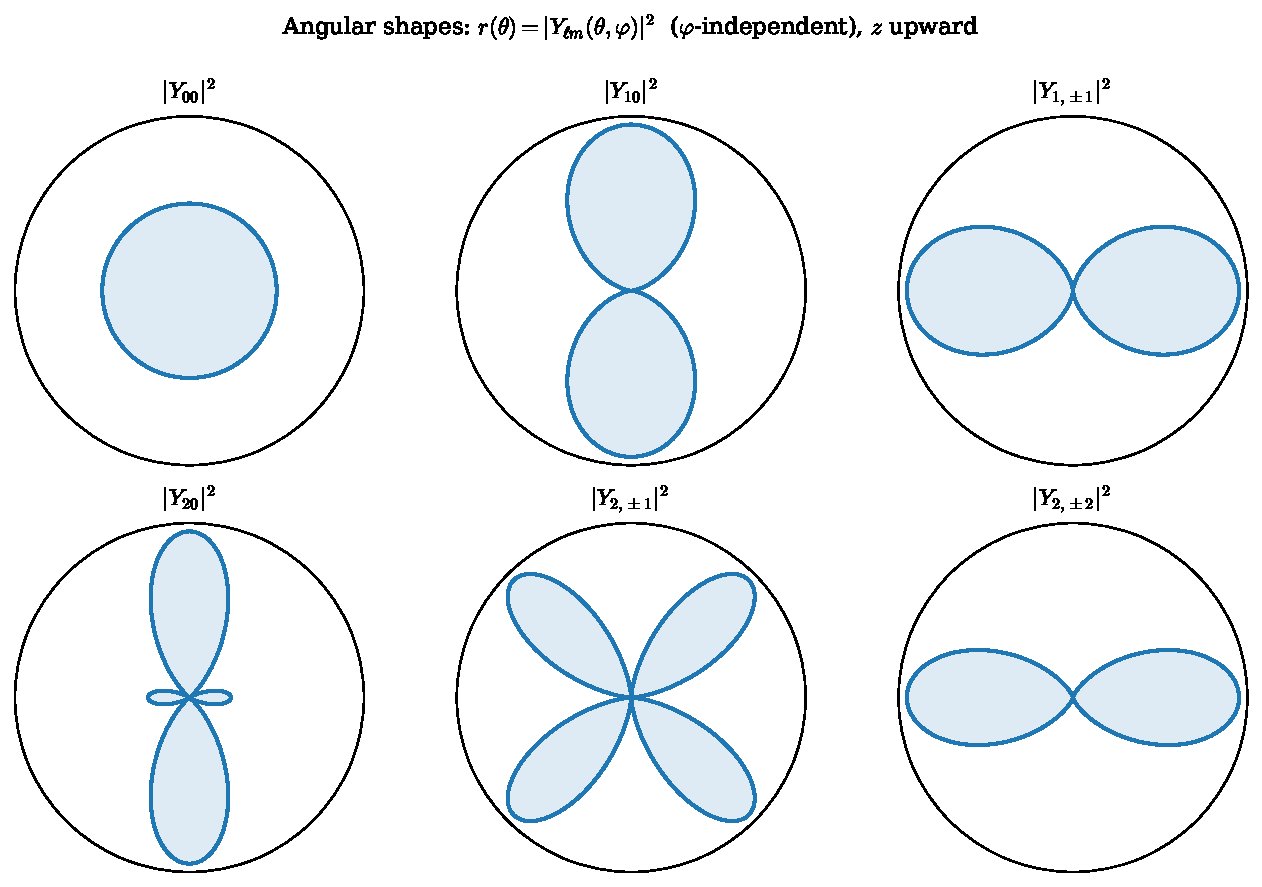
\includegraphics[width=0.9\textwidth]{fig_ylm.pdf}
  \caption{The integer catalogue on the sphere: angular probability
  profiles $|Y_{\ell m}(\theta)|^2$ through $\ell = 2$, exact
  closed forms, $z$ upward ($|Y_{\ell m}|^2$ is
  $\varphi$-independent, so the planar cut is the whole story).
  $\ell$ sets the angular structure; $m$ distributes it between pole
  and equator --- $|m| = \ell$ hugs the equator, $m = 0$ the axis.}
  \label{fig:ylm}
\end{figure}

\medskip
\noindent
The kinematics of rotation is now complete: the group
(\S\ref{sec:rotations}), its cover (\S\ref{sec:su2}), and every
stage it can play on \eqref{eq:J-catalogue}, with the spherical
harmonics as the integer towers' concrete realization. What is
missing is a \emph{dynamics} to put on the stage --- a Hamiltonian
that respects the rotations --- and the payoff for choosing one is
the hydrogen atom, the document's capstone.


%=======================================================================
\section{Central Potentials and Hydrogen}
%=======================================================================
\label{sec:hydrogen}

The document's threads converge here. The stage is
\S\ref{sec:J-spectrum}'s; the boundary-condition discipline and the
one-dimensional intuition are \S\ref{sec:one-dim}'s; the naming
scheme is \S\ref{sec:heisenberg-picture}'s CSCO; and the open
puzzle is
\S\ref{sec:classical-failures}'s --- an atom that should not exist,
emitting discrete lines with no classical origin. This section builds the
hydrogen atom from the Coulomb potential and answers that puzzle in
nanometers.

\subsection{Central potentials: three dimensions become one}
\label{sec:central}

Let $V = V(r)$: rotationally invariant, so $[\op H, \op{\vec L}] =
0$ --- angular momentum is conserved
(\S\ref{sec:heisenberg-picture}), and
$\{\op H, \op{\vec L}^2, \op L_z\}$ is a commuting set: the states
can carry the labels $(E, \ell, m)$ jointly. Separate accordingly.
In the position representation the kinetic operator splits into
radial and angular parts,
\begin{equation}
  -\hbar^2\nabla^2
  = -\,\hbar^2\,\frac1r\,\pd{^2}{r^2}\,r
  \;+\; \frac{\op{\vec L}^2}{r^2}
  \label{eq:laplacian-split}
\end{equation}
[the identity is a coordinate computation; stated, with the angular
part recognizable as $\op{\vec L}^2$ from \eqref{eq:Lz-polar} and
its siblings], so the ansatz
$\psi = R(r)\,Y_{\ell m}(\theta, \varphi)$ absorbs the angular
dependence entirely into \S\ref{sec:J-spectrum}'s eigenvalue
$\hbar^2\ell(\ell+1)$, and the substitution $u(r) = r\,R(r)$ lands
on
\begin{equation}
  \boxed{\;
  -\frac{\hbar^2}{2m}\,u''
  + \Bigl[
      V(r) + \frac{\hbar^2\,\ell(\ell+1)}{2m\,r^2}
    \Bigr] u
  = E\,u,
  \qquad
  u(0) = 0
  \;}
  \label{eq:radial-equation}
\end{equation}
--- a \emph{one-dimensional} Schr\"odinger problem on the half-line:
the whole of \S\ref{sec:one-dim} applies wholesale, with two new
fixtures. The boundary condition $u(0) = 0$ is a hard wall at the
origin ($R = u/r$ must stay finite --- the quick reason; the
airtight one: $u(0) \ne 0$ gives $R \sim 1/r$, and
$\nabla^2(1/r) = -4\pi\,\delta^3(\vx)$ plants a delta source the
equation cannot balance [stated]), so the origin is
\S\ref{sec:box}'s wall relocated; and the potential has acquired
the \emph{centrifugal barrier} --- the quantum version of the
classical $\ell^2/2mr^2$ of the central-force reduction
[Mech.\ \S3.3], with $\ell(\ell+1)$ where $\ell^2$ might have
been guessed (the ladder's $j(j+1)$, \eqref{eq:J-catalogue},
insists). States of higher $\ell$ are pushed off the origin; only
$\ell = 0$ states touch the nucleus.

\subsection{Hydrogen: scales first, then the spectrum}
\label{sec:hydrogen-spectrum}

The Coulomb problem is
$V(r) = -e^2/r$, with $e^2 \equiv q_e^2/4\pi\epsilon_0$ as
shorthand. Before solving anything, do what the house style demands:
ask what the parameters $(\hbar, m, e^2)$ can build. Exactly one
length and one energy can be built,
\begin{equation}
  a_0 = \frac{\hbar^2}{m e^2}
  \approx 0.529\,\text{\AA},
  \qquad
  \mathrm{Ry} = \frac{m e^4}{2\hbar^2}
  = \frac{e^2}{2 a_0}
  \approx 13.61\,\mathrm{eV}
  \label{eq:bohr-scales}
\end{equation}
--- and these are Example~\ref{ex:atomic-size}'s balance point made
exact: the radius where localization cost
($\sim \hbar^2/2ma_0^2$) and Coulomb gain ($\sim e^2/a_0$)
compete on equal terms. The atom's size was fixed by dimensional
analysis before a single equation; the equation's job is the
numerical coefficients and the \emph{pattern} of levels.

Solve \eqref{eq:radial-equation} in units $\rho = r/a_0$,
$\epsilon = E/\mathrm{Ry}$. The two ends dictate asymptotics ---
decay $u \sim \ee^{-\sqrt{-\epsilon}\,\rho}$ at infinity (bound
state), $u \sim \rho^{\ell+1}$ at the origin (imposed by the
centrifugal wall) --- so peel both off, $u = \rho^{\ell+1}\,
\ee^{-\sqrt{-\epsilon}\,\rho}\, w(\rho)$, and feed $w$ a power
series. The recursion that falls out relates consecutive
coefficients by
\begin{equation}
  \frac{c_{k+1}}{c_k}
  = \frac{2\bigl[\sqrt{-\epsilon}\,(k + \ell + 1) - 1\bigr]}
         {(k + 1)(k + 2\ell + 2)}
  \;\xrightarrow[k \to \infty]{}\;
  \frac{2\sqrt{-\epsilon}}{k} ,
\end{equation}
and the large-$k$ tail is the series of
$\ee^{+2\sqrt{-\epsilon}\,\rho}$: a non-terminating series
overwhelms the decay and the state fails to normalize --- the same
normalizability constraint that bounded \S\ref{sec:sho-spectrum}'s
ladder. Survival
requires \emph{termination}: some numerator must vanish,
$\sqrt{-\epsilon}\,(n_r + \ell + 1) = 1$ for a nonnegative integer
$n_r$, i.e., with $n \equiv n_r + \ell + 1$:
\begin{equation}
  \boxed{\;
  E_n = -\,\frac{\mathrm{Ry}}{n^2},
  \qquad n = 1, 2, 3, \dots,
  \qquad
  \ell \in \{0, 1, \dots, n-1\},
  \qquad
  \text{degeneracy } \sum_{\ell=0}^{n-1}(2\ell + 1) = n^2 .
  \;}
  \label{eq:hydrogen-spectrum}
\end{equation}

\begin{example}[Hydrogen's spectral lines in nanometers]
\label{ex:hydrogen-lines}
Section~\ref{sec:classical-failures} opened with spectral lines the
classical atom could not have; \S\ref{sec:stationary-states} showed
lines live at Bohr frequencies between levels; here are the levels,
so here are the lines. Between $n = 2$ and $n = 1$:
\begin{equation}
  \Delta E = \mathrm{Ry}\Bigl(1 - \tfrac14\Bigr)
  = 10.20\,\mathrm{eV}
  \qquad\Longrightarrow\qquad
  \lambda = \frac{hc}{\Delta E} = 121.5\,\mathrm{nm}
\end{equation}
--- Lyman-$\alpha$, the ultraviolet workhorse of astronomy. Between
$3$ and $2$: $\Delta E = 1.89\,\mathrm{eV}$, $\lambda =
656\,\mathrm{nm}$ --- H$\alpha$, \emph{the} red line of emission
nebulae, now a two-line computation. The whole zoo compresses to
the Rydberg formula
$1/\lambda = R_\infty(1/n_1^2 - 1/n_2^2)$ with
$R_\infty = \mathrm{Ry}/hc = 1.097\times10^7\,\mathrm m^{-1}$ ---
which derives the empirical rule of 1888, instantiates the
Rydberg--Ritz combination principle
(\S\ref{sec:stationary-states}), and answers the
document's opening puzzle in full, in the observed decimal
places. [Scope: nonrelativistic, spinless
electron, infinitely heavy proton --- the reduced-mass correction
is a factor $(1 + m_e/m_p)^{-1} \approx 1 - 1/1836$, already
visible in precision data, and fine structure needs the tools of
\S\S\ref{sec:addition}--\ref{sec:wigner-eckart} plus relativity;
stated.]
\end{example}

\subsection{The radial catalogue}
\label{sec:radial-functions}

Termination at $n_r = n - \ell - 1$ makes $w$ a polynomial of that
degree (an associated Laguerre polynomial [normalization stated]),
so the radial function $R_{n\ell}$ has exactly $n - \ell - 1$ nodes
--- the oscillation theorem of \S\ref{sec:box} passing its check in
the radial column. The low family, explicitly ($\rho = r/a_0$, in
units $a_0^{-3/2}$):
\begin{equation}
  R_{10} = 2\,\ee^{-\rho},
  \qquad
  R_{20} = \frac{2 - \rho}{2\sqrt2}\,\ee^{-\rho/2},
  \qquad
  R_{21} = \frac{\rho}{2\sqrt6}\,\ee^{-\rho/2},
\end{equation}
and Fig.~\ref{fig:hydrogen} draws the radial probability densities
$P_{n\ell} = r^2|R_{n\ell}|^2$ through $n = 3$. Three features to
read off: the ground state peaks at exactly $r = a_0$ (differentiate
$\rho^2\ee^{-2\rho}$); size grows quadratically, $\langle r\rangle
\sim n^2 a_0$ --- Rydberg atoms are \emph{large}; and at fixed $n$,
higher $\ell$ means fewer radial nodes but a stronger centrifugal
push off the origin --- the $(3,0)$ state touches the nucleus, the
$(3,2)$ state cannot, a distinction that controls everything from
hyperfine structure to which orbitals chemistry builds bonds with.

\begin{figure}[htbp]
  \centering
  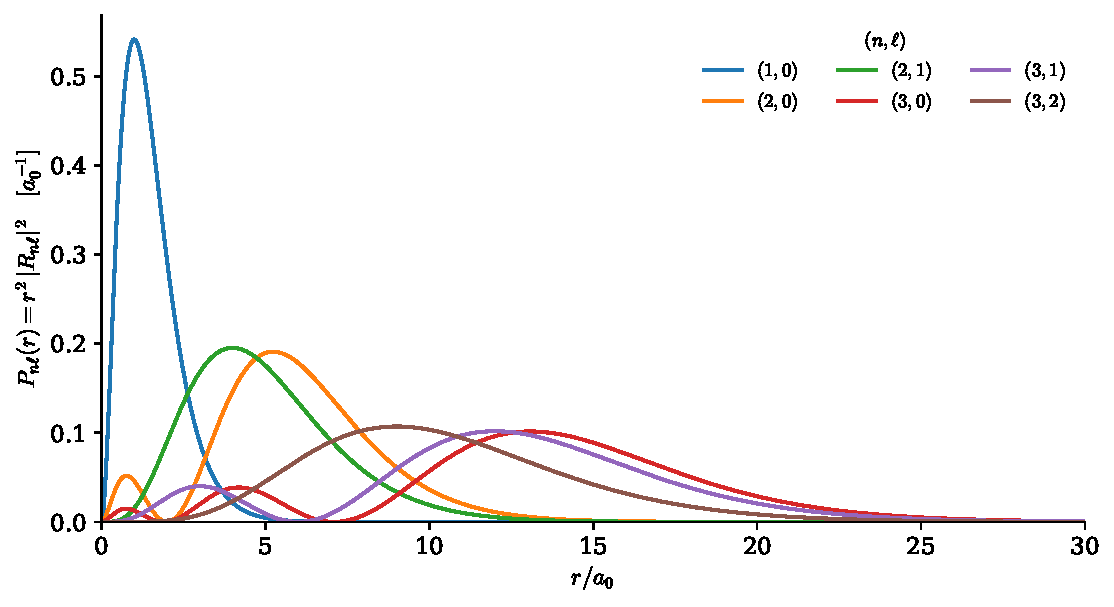
\includegraphics[width=0.82\textwidth]{fig_hydrogen.pdf}
  \caption{Hydrogen's radial probability densities
  $P_{n\ell}(r) = r^2|R_{n\ell}|^2$ through $n = 3$, exact closed
  forms; each curve numerically verified to unit norm by the figure
  script. Node count
  $n - \ell - 1$; ground-state peak at exactly $a_0$; the $n^2$
  growth of size; the centrifugal exclusion of high-$\ell$ states
  from the origin.}
  \label{fig:hydrogen}
\end{figure}

\begin{remark}[The degeneracy is not an accident --- it is a bigger
symmetry]\label{rem:runge-lenz}
Rotational symmetry explains the $(2\ell + 1)$-fold degeneracy in
$m$ --- states of one $\ell$-tower are rotations of each other ---
but it does \emph{not} explain why $\ell = 0, \dots, n{-}1$ all
land on the same $E_n$: a generic central potential splits them,
and \eqref{eq:hydrogen-spectrum}'s $n^2$ is special to $1/r$. The
classical fingerprint of the same specialness is that Coulomb
orbits \emph{close} (ellipses that do not precess --- a property
$1/r$ shares only with $r^2$ [stated; Bertrand's theorem]), and
closed orbits mean an extra conserved quantity: the Runge--Lenz
vector, pointing along the ellipse's fixed axis. Quantum
mechanically the corresponding operator commutes with $\op H$, and
together with $\op{\vec L}$ it closes a \emph{larger} algebra ---
$SO(4)$, rotations of a four-dimensional space --- whose
representation theory delivers exactly the $n^2$-dimensional
multiplets [stated; one of the subject's classic algebraic
solutions, Pauli 1926]. The moral is the document's in miniature:
where there is an unexplained degeneracy, look for the symmetry
that explains it.
\end{remark}

\medskip
\noindent
One atom is built. But the electron has spin the capstone ignored,
and real atoms have more than one angular momentum to their name
--- orbital and spin, electron and nucleus. Composing them is not
optional bookkeeping; it is where the tensor product of
\S\ref{sec:tensor-product} finally does physics, and it is next.


%=======================================================================
\section{Addition of Angular Momenta}
%=======================================================================
\label{sec:addition}

The hydrogen capstone ended on a confession: the electron carries a
spin the calculation ignored, so even one hydrogen atom holds
\emph{two} angular momenta --- $\op{\vec L}$ of the orbit,
$\op{\vec S}$ of the electron --- and nature's Hamiltonians couple
them. This section works out what ``the total angular momentum of a
composite'' means and what values it can take. The material has a
reputation for abstraction, so the treatment is deliberately slow:
the \emph{problem} is stated before the machinery, the commutator
computation that creates the two-bases problem is displayed in full
rather than left at [stated] level, and
the simplest nontrivial case is then worked out completely.

\subsection{A careful statement of the problem}
\label{sec:addition-problem}

Two subsystems with angular momenta $j_1$ and $j_2$ live, by
\S\ref{sec:tensor-product}, on the tensor product
\begin{equation}
  \mathcal H = \mathcal H_1 \otimes \mathcal H_2,
  \qquad
  \dim \mathcal H = (2j_1 + 1)(2j_2 + 1),
\end{equation}
with the obvious product basis
$\ket{j_1 m_1}\otimes\ket{j_2 m_2} \equiv \ket{m_1, m_2}$ (the
$j$'s fixed throughout, suppressed when unambiguous). Each factor
carries its own generators, acting only on its own slot ---
$\op{\vec J}_1 \otimes \idop$ and $\idop \otimes \op{\vec J}_2$,
written $\op{\vec J}_1$, $\op{\vec J}_2$ for short --- and because
they touch different slots they commute with each other:
$[\op J_{1i}, \op J_{2k}] = 0$, always.

Now rotate the \emph{whole} system. A rotation turns both parts at
once, $U(R) = U_1(R)\otimes U_2(R)$, and expanding each factor to
first order (\eqref{eq:J-generator}, twice) shows the composite's
generator is the sum:
\begin{equation}
  \op{\vec J} \;\equiv\; \op{\vec J}_1 + \op{\vec J}_2
  \qquad\text{(meaning }
  \op{\vec J}_1\otimes\idop + \idop\otimes\op{\vec J}_2\text{)}.
\end{equation}
This is what ``adding angular momenta'' means --- not a numerical
addition but an operator sum on a tensor product --- and the first
sanity check is that the sum still \emph{is} an angular momentum:
\begin{equation}
  [\op J_i, \op J_k]
  = [\op J_{1i}, \op J_{1k}] + [\op J_{2i}, \op J_{2k}]
  = \ii\hbar\,\epsilon_{ikl}
    \bigl(\op J_{1l} + \op J_{2l}\bigr)
  = \ii\hbar\,\epsilon_{ikl}\,\op J_l
  \label{eq:sum-is-J}
\end{equation}
(the cross terms vanish --- different slots), so the entire
catalogue \eqref{eq:J-catalogue} applies to $\op{\vec J}$: its
representation content is some collection of $(j, m)$ towers. The
question of the section: \emph{which} towers, and how they sit
inside the product basis.

Here is why the question has content. There are now two natural
complete sets of commuting observables:
\begin{center}
\begin{tabular}{ll}
\toprule
\emph{uncoupled} set & \emph{coupled} set \\
\midrule
$\op{\vec J}_1^{\,2},\ \op{\vec J}_2^{\,2},\
\op J_{1z},\ \op J_{2z}$
& $\op{\vec J}_1^{\,2},\ \op{\vec J}_2^{\,2},\
\op{\vec J}^{\,2},\ \op J_z$ \\[2pt]
basis $\ket{m_1, m_2}$ & basis $\ket{j, m}$ \\[2pt]
answers: each part's $z$-component
& answers: the total's magnitude and $z$-component \\
\bottomrule
\end{tabular}
\end{center}
Both are legitimate; they answer different experimental questions;
and they are \emph{different bases}, because the coupled set's
$\op{\vec J}^{\,2}$ refuses to commute with the uncoupled set's
$\op J_{1z}$. That refusal is the crux of the whole subject, so it
deserves its computation. Expand
\begin{equation}
  \op{\vec J}^{\,2}
  = \op{\vec J}_1^{\,2} + \op{\vec J}_2^{\,2}
    + 2\,\op{\vec J}_1\!\cdot\op{\vec J}_2 ,
  \label{eq:J2-expansion}
\end{equation}
note the first two terms commute with everything in sight, and hit
the cross term:
\begin{equation}
  \bigl[\op{\vec J}_1\!\cdot\op{\vec J}_2,\ \op J_{1z}\bigr]
  = [\op J_{1x}, \op J_{1z}]\,\op J_{2x}
  + [\op J_{1y}, \op J_{1z}]\,\op J_{2y}
  = \ii\hbar\bigl(
      \op J_{1x}\op J_{2y} - \op J_{1y}\op J_{2x}
    \bigr)
  \;\ne\; 0
  \label{eq:crux-commutator}
\end{equation}
(only slot-1 operators feel the commutator; the result is the
$z$-component of $\op{\vec J}_1\times\op{\vec J}_2$). Physically:
the total magnitude involves the \emph{relative orientation} of the
two spins, and pinning down one spin's $z$-component disturbs
exactly that. So sharp $(m_1, m_2)$ and sharp $(j, m)$ are
incompatible bookkeeping --- two adapted coordinate systems
(Remark~\ref{rem:adapted-coordinates-qm}, once more) for one space,
and the change of basis between them is this section's deliverable.

Two members are shared: $\op J_z = \op J_{1z} + \op J_{2z}$
commutes with both sets, and acting on a product state,
\begin{equation}
  \op J_z\ket{m_1, m_2}
  = \hbar\,(m_1 + m_2)\ket{m_1, m_2}
  \qquad\Longrightarrow\qquad
  m = m_1 + m_2 :
  \label{eq:m-additive}
\end{equation}
the $z$-components \emph{do} add numerically. This one additive
quantum number is the crack through which the whole structure can
be pried open.

\subsection{Which totals occur: counting by $m$}
\label{sec:m-counting}

Since every $j$-tower contributes exactly one state at each $m \in
\{-j, \dots, j\}$, the multiplicities $N(m)$ --- how many product
states carry a given total $m$ --- determine the tower content
completely: the number of towers whose top rung is at $m$ is
$N(m) - N(m+1)$. And $N(m)$ is elementary counting on
\eqref{eq:m-additive}: the number of ways to write
$m = m_1 + m_2$ with $|m_1| \le j_1$, $|m_2| \le j_2$.

Count it for a concrete case first, $j_1 = 1$, $j_2 = \tfrac12$
(six product states):
\begin{center}
\begin{tabular}{c|l|c}
\toprule
$m$ & product states $(m_1, m_2)$ & $N(m)$ \\
\midrule
$+\tfrac32$ & $(1, +\tfrac12)$ & 1 \\
$+\tfrac12$ & $(1, -\tfrac12),\ (0, +\tfrac12)$ & 2 \\
$-\tfrac12$ & $(0, -\tfrac12),\ (-1, +\tfrac12)$ & 2 \\
$-\tfrac32$ & $(-1, -\tfrac12)$ & 1 \\
\bottomrule
\end{tabular}
\end{center}
Read the staircase top-down: one tower tops out at
$m = \tfrac32$ (so $j = \tfrac32$ occurs, once), one more appears at
$m = \tfrac12$ ($N$ jumped $1 \to 2$: a $j = \tfrac12$ tower), and
then nothing new --- $N$ never exceeds 2. Conclusion:
$1 \otimes \tfrac12 = \tfrac32 \oplus \tfrac12$, dimensions
$6 = 4 + 2$. The general case is the same staircase: $N(m)$ starts
at $1$ for $m = j_1 + j_2$, climbs by one per step down, and
plateaus once the shorter ladder is exhausted --- at
$m = |j_1 - j_2|$, after which no new towers appear. Hence the
\emph{triangle rule}:
\begin{equation}
  \boxed{\;
  j_1 \otimes j_2
  = \bigoplus_{j = |j_1 - j_2|}^{\,j_1 + j_2} j,
  \qquad
  \text{each } j \text{ exactly once,}
  \;}
  \label{eq:triangle-rule}
\end{equation}
the possible totals being exactly the triangle-compatible values
--- the quantum shadow of the classical fact that two vectors of
lengths $j_1, j_2$ compose to anything between $|j_1 - j_2|$ and
$j_1 + j_2$, discretized in unit steps. The dimension check is a
telescoping sum worth displaying once:
\begin{equation}
  \sum_{j = |j_1 - j_2|}^{j_1 + j_2} (2j + 1)
  = (j_1 + j_2 + 1)^2 - (j_1 - j_2)^2
  = (2j_1 + 1)(2j_2 + 1)
  \;\checkmark
\end{equation}
(each $2j + 1$ is a difference of consecutive squares,
$(j+1)^2 - j^2$; the sum collapses to its endpoints).

\subsection{Clebsch--Gordan coefficients: the change of adapted
coordinates}\label{sec:CG}

The two bases are related by a unitary matrix whose entries have a
name:
\begin{equation}
  \ket{j, m}
  = \sum_{m_1 + m_2 = m}
    \underbrace{\braket{m_1, m_2}{j, m}}_{\text{Clebsch--Gordan
    coefficient}}
    \;\ket{m_1, m_2},
  \label{eq:CG-def}
\end{equation}
the sum restricted by \eqref{eq:m-additive} --- the one selection
rule every coefficient obeys for free. Nothing about them is new
machinery: \eqref{eq:CG-def} is a change of basis exactly as in
\S\ref{sec:adapted-coordinates}, computable in every case by the
two tools already in hand --- \emph{ladders} ($\op J_\pm =
\op J_{1\pm} + \op J_{2\pm}$ walks down a tower once its top is
known, and the top of the top tower is unmissable:
$\ket{j_1 + j_2,\, j_1 + j_2} = \ket{j_1, j_2}$, the unique maximal
state) --- and \emph{orthogonality} (each new tower's top is fixed,
up to phase, by being orthogonal to everything already built at its
$m$). Conventional phases (Condon--Shortley: all coefficients real,
and the highest-$m_1$ coefficient in each tower positive) pin the
remaining signs [stated]; beyond that there is nothing to memorize,
only an algorithm --- run explicitly in the next subsection --- and
a lookup habit: Appendix~\ref{app:cg-tables} tabulates the small
products, every entry machine-generated and verified.

\subsection{The complete worked case: $\tfrac12 \otimes \tfrac12$}\label{sec:half-half}

Two spin-$\tfrac12$'s: four product states $\ket{++}, \ket{+-},
\ket{-+}, \ket{--}$, and the triangle rule
\eqref{eq:triangle-rule} promises $\tfrac12\otimes\tfrac12 = 1
\oplus 0$: a \emph{triplet} and a \emph{singlet}, $4 = 3 + 1$.

\emph{Step 1: the top.} The maximal state is the unique $m = 1$
state:
\begin{equation}
  \ket{1, 1} = \ket{++}.
\end{equation}

\emph{Step 2: ladder down, factors and all.} Apply $\op J_- =
\op J_{1-} + \op J_{2-}$. On the left, the catalogue's matrix
element \eqref{eq:J-catalogue} with $j = 1$, $m = 1$:
$\op J_-\ket{1,1} = \hbar\sqrt{1\cdot2 - 1\cdot0}\,\ket{1,0}
= \hbar\sqrt2\,\ket{1, 0}$. On the right, each one-particle
lowering carries $\hbar\sqrt{\frac12\cdot\frac32 -
\frac12\cdot(-\frac12)} = \hbar$:
\begin{equation}
  \bigl(\op J_{1-} + \op J_{2-}\bigr)\ket{++}
  = \hbar\,\ket{-+} + \hbar\,\ket{+-}.
\end{equation}
Equate and divide by $\hbar\sqrt2$:
\begin{equation}
  \ket{1, 0}
  = \frac{1}{\sqrt2}\bigl(\ket{+-} + \ket{-+}\bigr).
\end{equation}
Once more: $\op J_-\ket{1,0} = \hbar\sqrt2\,\ket{1,-1}$, while the
right side gives $\hbar(\ket{--} + \ket{--})/\sqrt2 =
\hbar\sqrt2\,\ket{--}$, so $\ket{1,-1} = \ket{--}$ --- the ladder
closes exactly where the catalogue said it must.

\emph{Step 3: the leftover.} Four states, three used. The $m = 0$
subspace is two-dimensional and the triplet took one direction; the
orthogonal complement, normalized and with the conventional phase,
is
\begin{equation}
  \ket{0, 0}
  = \frac{1}{\sqrt2}\bigl(\ket{+-} - \ket{-+}\bigr)
  \qquad\text{--- the \emph{singlet}.}
\end{equation}

\emph{Step 4: verify the labels.} That $\ket{0,0}$ really has
$j = 0$ should be \emph{checked}, not trusted, and the check
exercises the machinery. First rewrite the cross term of
\eqref{eq:J2-expansion} in ladder form --- one line,
\begin{equation}
  \op J_{1+}\op J_{2-} + \op J_{1-}\op J_{2+}
  = 2\bigl(\op J_{1x}\op J_{2x} + \op J_{1y}\op J_{2y}\bigr)
  \;\Longrightarrow\;
  \op{\vec J}_1\!\cdot\op{\vec J}_2
  = \op J_{1z}\op J_{2z}
  + \tfrac12\bigl(
      \op J_{1+}\op J_{2-} + \op J_{1-}\op J_{2+}
    \bigr),
  \label{eq:dot-ladder}
\end{equation}
then evaluate on the singlet, term by term. The $z z$ term gives
$(\tfrac\hbar2)(-\tfrac\hbar2) = -\tfrac{\hbar^2}4$ on both
$\ket{+-}$ and $\ket{-+}$. The ladder terms swap the spins with a
factor $\hbar^2$ each ($\op J_{1-}\op J_{2+}\ket{+-} =
\hbar^2\ket{-+}$, $\op J_{1+}\op J_{2-}\ket{-+} = \hbar^2\ket{+-}$,
the other orderings annihilate), so on the antisymmetric
combination the swap costs a sign:
\begin{equation}
  \op{\vec J}_1\!\cdot\op{\vec J}_2\,\ket{0,0}
  = \Bigl(-\frac{\hbar^2}{4} - \frac{\hbar^2}{2}\Bigr)\ket{0,0}
  = -\frac{3\hbar^2}{4}\,\ket{0,0},
\end{equation}
and assembling \eqref{eq:J2-expansion} with
$\op{\vec J}_{1,2}^{\,2} = \tfrac34\hbar^2$:
\begin{equation}
  \op{\vec J}^{\,2}\ket{0,0}
  = \Bigl(\tfrac34 + \tfrac34 - \tfrac32\Bigr)\hbar^2\,\ket{0,0}
  = 0
  \;\checkmark
\end{equation}
--- and the same evaluation on $\ket{1,0}$ (swap costs no sign)
gives $+\tfrac{\hbar^2}4 + \tfrac{\hbar^2}2$, hence
$\op{\vec J}^{\,2} = 2\hbar^2 = 1(1{+}1)\hbar^2$ $\checkmark$. The
summary table, with every entry now derived:
\begin{center}
\begin{tabular}{lcc}
\toprule
state & $(j, m)$ & $\op{\vec J}_1\!\cdot\op{\vec J}_2 / \hbar^2$ \\
\midrule
$\ket{++}$ & $(1, +1)$ & $+\tfrac14$ \\
$\tfrac{1}{\sqrt2}(\ket{+-} + \ket{-+})$ & $(1, 0)$ & $+\tfrac14$ \\
$\ket{--}$ & $(1, -1)$ & $+\tfrac14$ \\
$\tfrac{1}{\sqrt2}(\ket{+-} - \ket{-+})$ & $(0, 0)$ & $-\tfrac34$ \\
\bottomrule
\end{tabular}
\end{center}
The last column is the section's most-used practical output: any
Hamiltonian containing $\op{\vec J}_1\!\cdot\op{\vec J}_2$ --- and
nature's spin--spin couplings do --- is \emph{diagonal} in the
coupled basis, constant on each multiplet, splitting singlet from
triplet by $\hbar^2$.

\begin{example}[The algorithm scales: $\tfrac32 \otimes \tfrac12$]
\label{ex:three-half}
Re-run the machine, compactly, on the next case up --- eight
product states $\ket{m_1, m_2}$, $m_1 \in \{\pm\tfrac32,
\pm\tfrac12\}$, $m_2 = \pm\tfrac12$. First the staircase:
\begin{center}
\begin{tabular}{c|l|c}
\toprule
$m$ & product states & $N(m)$ \\
\midrule
$+2$ & $(\tfrac32, +\tfrac12)$ & 1 \\
$+1$ & $(\tfrac32, -\tfrac12),\ (\tfrac12, +\tfrac12)$ & 2 \\
$0$ & $(\tfrac12, -\tfrac12),\ (-\tfrac12, +\tfrac12)$ & 2 \\
$-1$ & $(-\tfrac12, -\tfrac12),\ (-\tfrac32, +\tfrac12)$ & 2 \\
$-2$ & $(-\tfrac32, -\tfrac12)$ & 1 \\
\bottomrule
\end{tabular}
\end{center}
One tower tops at $m = 2$, one new one at $m = 1$, none after:
$\tfrac32 \otimes \tfrac12 = 2 \oplus 1$, dimensions $8 = 5 + 3$,
as \eqref{eq:triangle-rule} promised. Now two rows of coefficients,
by the same two tools. \emph{Ladder}: $\ket{2,2} =
\ket{\tfrac32, +\tfrac12}$, and applying $\op J_-$ --- left side
$\hbar\sqrt{2\cdot3 - 2\cdot1}\,\ket{2,1} = 2\hbar\,\ket{2,1}$,
right side $\hbar\sqrt3\,\ket{\tfrac12, +\tfrac12} +
\hbar\,\ket{\tfrac32, -\tfrac12}$ (the $\sqrt3$ from
\eqref{eq:J-catalogue} at $j_1 = \tfrac32$, $m_1 = \tfrac32$;
the $\hbar$ from the spin-$\tfrac12$ slot) --- gives
\begin{equation}
  \ket{2, 1}
  = \frac{\sqrt3}{2}\,\ket{\tfrac12, +\tfrac12}
  + \frac12\,\ket{\tfrac32, -\tfrac12}.
\end{equation}
\emph{Orthogonality}: the $m = 1$ subspace is two-dimensional and
the $j = 2$ tower has claimed one direction; the $j = 1$ tower's
top is the complement, with the overall sign fixed by the
Condon--Shortley convention --- \emph{the coefficient of the
highest-$m_1$ state is positive}:
\begin{equation}
  \ket{1, 1}
  = \frac{\sqrt3}{2}\,\ket{\tfrac32, -\tfrac12}
  - \frac12\,\ket{\tfrac12, +\tfrac12},
\end{equation}
and continued lowering fills in the rest --- nothing new happens,
only more square roots. The case is not academic: a nucleus of spin
$\tfrac32$ coupled to an electron spin is exactly this
decomposition, and the two hyperfine levels $F = 2, 1$ of
$^{87}$Rb's ground state --- the pair between which laser cooling
and atomic-clock physics runs --- are these two towers [stated].
\end{example}

\begin{remark}[The entanglement flag delivered]
\label{rem:singlet-entangled}
Section~\ref{sec:tensor-product} flagged that most states of a
composite are entangled and promised a physical specimen. The
singlet is \emph{the} specimen: $\ket{0,0}$ is manifestly not a
product (try $(a\ket+ + b\ket-)\otimes(c\ket+ + d\ket-)$: matching
coefficients forces $ac = bd = 0$ against $ad = -bc \ne 0$), and
its correlations are total --- measure either spin along \emph{any}
axis and the other is fixed opposite, since $j = 0$ makes the state
invariant under the simultaneous rotation $U\otimes U$ (no
direction is special: a rotationally invariant state has no Bloch
vector to point). This is the two-particle state of the
Einstein--Podolsky--Rosen discussion and of Bell's inequalities
[stated; the flag planted in \S\ref{sec:tensor-product} is delivered
to exactly this depth and the literature does the rest], and it was
built here by nothing more exotic than a ladder and an
orthogonality.
\end{remark}

\begin{example}[The 21-centimeter line]
\label{ex:21cm}
Hydrogen's ground state, $(n, \ell) = (1, 0)$, carries two idle
spins: the electron's and the proton's. Their magnetic coupling is
proportional to $\op{\vec S}_e\!\cdot\op{\vec S}_p$ --- so the
table above \emph{is} the level diagram: a triplet and a singlet,
split by the hyperfine interaction, singlet lower. The measured
splitting is tiny,
\begin{equation}
  \Delta E = 5.87\,\mu\mathrm{eV},
  \qquad
  f = \Delta E/h = 1420.4\,\mathrm{MHz},
  \qquad
  \lambda = 21.1\,\mathrm{cm}
\end{equation}
[experimental input; predicting $\Delta E$'s magnitude needs the
magnetic moments and the contact interaction --- note it involves
$|\psi(0)|^2$, nonzero only for the $\ell = 0$ states of
Fig.~\ref{fig:hydrogen} --- stated], corresponding to
$\Delta E/k_B \approx 68\,\mathrm{mK}$: any astrophysical
environment populates the triplet, and the slow magnetic-dipole
decay back to the singlet emits the \emph{21-centimeter line} ---
the radio signature by which neutral hydrogen is mapped across
galaxies, including the first maps of the Milky Way's spiral arms.
The structure of that line --- why there are exactly two levels
with statistical weights $3 : 1$ --- is precisely the four-row
table derived above; radio astronomy runs on a Clebsch--Gordan
decomposition.
\end{example}

\medskip
\noindent
The composition of \emph{states} is settled: totals by the triangle
rule, bases by ladders and orthogonality. What remains for the
symmetry story is the composition of states with \emph{operators}
--- how observables themselves transform under rotation, and the
theorem that squeezes every rotational matrix element through one
reduced number. That theorem is next.


%=======================================================================
\section{Tensor Operators and the Wigner--Eckart Theorem}
%=======================================================================
\label{sec:wigner-eckart}

One asymmetry remains in the symmetry story. States have been
sorted into rotation multiplets --- the $(j, m)$ towers --- but
\emph{operators} have not, and physical predictions end in
matrix elements $\bra{\beta}\op A\ket{\alpha}$ with an operator in
the middle. This closing technical section repairs the asymmetry,
carefully: it defines what it means for an operator to transform,
discovers that operators fall into the \emph{same} towers as
states, and proves --- to the depth of one displayed
recursion --- the theorem that then squeezes every rotational
matrix element in atomic physics through a single number. The
abstraction is front-loaded; the payoff, at the end, is as concrete
as which spectral lines exist.

\subsection{How operators transform}
\label{sec:operator-transform}

Rotate the system: states go $\ket\psi \to U\ket\psi$. For an
operator, ``transform'' means whatever keeps the bookkeeping
consistent, and expectation values dictate it: the rotated
experiment measures $\bra\psi U^\dagger\,\op A\,U\ket\psi$, so the
operator's transform is $\op A \to U^\dagger \op A\, U$. Now impose
physics on specific operators. The position operator is a
\emph{vector}: rotating the apparatus must rotate its readings,
\begin{equation}
  U^\dagger(R)\;\op q_i\;U(R) = R_{ik}\,\op q_k .
  \label{eq:vector-finite}
\end{equation}
Feed in an infinitesimal rotation
\eqref{eq:J-generator} about $\hat n$: the left side is
$\op q_i + \tfrac{\ii}{\hbar}\,\dd\varphi\,[\hat n\cdot\op{\vec J},
\op q_i]$, the right side is
$\op q_i + \dd\varphi\,(\hat n\times\op{\vec q})_i$, and matching
--- for every axis --- gives the commutator form of
``vectorhood'':
\begin{equation}
  \boxed{\;
  [\op J_i, \op V_k] = \ii\hbar\,\epsilon_{ikl}\,\op V_l
  \;}
  \qquad\text{(vector operator)},
  \qquad
  [\op J_i, \op S\,] = 0
  \quad\text{(scalar operator)}.
  \label{eq:vector-def}
\end{equation}
This is a \emph{definition by commutators}, and it already has
instances: $\op{\vec q}$, $\op{\vec p}$, $\op{\vec L}$,
$\op{\vec S}$ all satisfy it (for $\op{\vec L}$ it is
\eqref{eq:J-algebra} itself), while $\op{\vec q}\cdot\op{\vec p}$,
$\op{\vec q}^{\,2}$, $\op H_{\text{central}}$ are scalars. Notice
what \eqref{eq:vector-def} formally \emph{is}: the statement that
the components $\op V_k$, under the adjoint action of
$\op{\vec J}$ (action by commutator), shuffle among themselves
exactly the way a $j = 1$ triple of states would. That observation
--- operators organize into the same multiplets as states --- is
the entire section in embryo, and making it precise is next.

\subsection{Cartesian tensors: the obvious generalization and its
redundancy}\label{sec:cartesian-tensors}

Given \eqref{eq:vector-def}, the natural next move is more indices.
Define a \emph{Cartesian tensor} of rank $n$ as an object with $n$
vector indices, transforming with one rotation matrix per index ---
constructively, take products of vectors: the \emph{dyadic}
\begin{equation}
  \op T_{ik} = \op U_i \op V_k,
  \qquad
  U^\dagger\,\op T_{ik}\,U
  = R_{ii'}\,R_{kk'}\;\op T_{i'k'},
  \label{eq:dyadic}
\end{equation}
nine components, and the pattern continues to any rank. This is the
tensor grammar of the field-theory notes [Fld.\ \S3.7], imported to
operator components, and it is perfectly \emph{correct}. It is
also, as an organizing scheme, \emph{redundant} --- and watching
the redundancy is the fastest route to the right definition. Split
the dyadic identically into three pieces:
\begin{equation}
  \op U_i \op V_k
  = \underbrace{\frac{\op{\vec U}\!\cdot\op{\vec V}}{3}\,
    \delta_{ik}}_{\text{trace: } 1}
  \;+\;
  \underbrace{\frac{\op U_i \op V_k - \op U_k \op V_i}{2}}_{%
    \text{antisymmetric: } 3}
  \;+\;
  \underbrace{\Bigl(
    \frac{\op U_i \op V_k + \op U_k \op V_i}{2}
    - \frac{\op{\vec U}\!\cdot\op{\vec V}}{3}\,\delta_{ik}
  \Bigr)}_{\text{symmetric traceless: } 5}
  \label{eq:cartesian-decomposition}
\end{equation}
(an identity --- add the three terms and cancel). Now rotate. Each
block stays strictly within itself, for a transparent reason each:
the trace is a scalar because $R\,\delta\,R^{\mathsf T} = \delta$
--- the \emph{defining equation} of the rotation group, [Fld.\
\S3.1]'s template once more; the antisymmetric part packages as a
vector, $\tfrac12\epsilon_{ikl}(\op U_k\op V_l - \op U_l\op V_k) =
(\op{\vec U}\times\op{\vec V})_i$, and vectors rotate among
themselves; and symmetry-plus-tracelessness survives conjugation by
any $R$. So the nine components never mix as nine: rotations act on
\eqref{eq:cartesian-decomposition} block-diagonally, in pieces of
size
\begin{equation}
  3 \times 3 = 1 + 3 + 5 .
  \label{eq:one-three-five}
\end{equation}
The Cartesian packaging is \emph{reducible}: it lumps together
subspaces that never speak to one another, like insisting on one
$9\times9$ matrix where three small blocks act. The counts $1, 3,
5$ are a broad hint --- they are $2k + 1$ for $k = 0, 1, 2$, the
dimensions of the state catalogue \eqref{eq:J-catalogue} --- and
they pose the section's real question: what are the \emph{minimal}
rotation-closed operator families, the irreducible pieces the
Cartesian language keeps bundling?

\subsection{Spherical tensors: the irreducible organization}
\label{sec:spherical-tensors}

The answer's shape is already in hand. Irreducible multiplets of the
rotation algebra are the $(2k{+}1)$-component towers of
\S\ref{sec:J-spectrum}, laddered by $\op J_\pm$ and graded by
$\op J_z$; demand operator families organized the same way. Define
a \emph{spherical tensor of rank $k$} as any $2k{+}1$ operators
$\op T^{(k)}_q$, $q = -k, \dots, k$, obeying
\begin{equation}
  \boxed{\;
  [\op J_z, \op T^{(k)}_q] = \hbar\, q\;\op T^{(k)}_q,
  \qquad
  [\op J_\pm, \op T^{(k)}_q]
  = \hbar\sqrt{k(k+1) - q(q\pm1)}\;\op T^{(k)}_{q\pm1}
  \;}
  \label{eq:tensor-def}
\end{equation}
--- the catalogue's matrix elements \eqref{eq:J-catalogue},
transplanted verbatim from action-on-states to
action-by-commutator: \emph{an operator multiplet is a tower that
commutators ladder}. (Equivalently, in finite form, the components
mix by the $\mathscr D^{(k)}$-matrices of \S\ref{sec:D-functions};
the infinitesimal version \eqref{eq:tensor-def} is taken as the
definition because it is convention-proof and computation-ready.
That the adjoint action is a legitimate ``action'' at all --- that
acting by nested commutators obeys the same algebra --- is the
Jacobi identity of \S\ref{sec:brackets-commutators}, invoked one
last time.)

A scalar is the $k = 0$ case. A vector fits with the spherical
repackaging
\begin{equation}
  \op V^{(1)}_0 = \op V_z,
  \qquad
  \op V^{(1)}_{\pm1}
  = \mp\,\frac{\op V_x \pm \ii\,\op V_y}{\sqrt2},
  \label{eq:spherical-components}
\end{equation}
and one check shows the definition engaging: using
\eqref{eq:vector-def},
\begin{equation}
  [\op J_z,\ \op V^{(1)}_{+1}]
  = -\frac{[\op J_z, \op V_x] + \ii\,[\op J_z, \op V_y]}{\sqrt2}
  = -\frac{\ii\hbar\,\op V_y + \hbar\,\op V_x}{\sqrt2}
  = \hbar\;\op V^{(1)}_{+1}
  \quad\checkmark
\end{equation}
--- eigenvalue $q = +1$, as \eqref{eq:tensor-def} demands (the
$\op J_\pm$ relations check the same way). The paradigm rank-$k$
example: the spherical harmonics themselves, read as multiplication
operators, $Y_{km}(\hat{\op q})$ --- they were \emph{built} as
$(k, m)$ towers in \S\ref{sec:orbital-integers}.

Now return to the dyadic and name its blocks in the new language.
The counts \eqref{eq:one-three-five} identify the three pieces of
\eqref{eq:cartesian-decomposition} as spherical tensors of ranks
$0, 1, 2$ --- dot product, cross product, and \emph{quadrupole} ---
so the decomposition every linear-algebra student knows (trace,
antisymmetric, symmetric-traceless) is a Clebsch--Gordan statement
about operators,
\begin{equation}
  1 \otimes 1 = 0 \oplus 1 \oplus 2,
\end{equation}
with the triangle rule \eqref{eq:triangle-rule} presiding, exactly
as it did for composite states. Two morals. First, \emph{Cartesian
tensors are reducible; spherical tensors are their irreducible
pieces} --- the spherical language is not a rival convention but
the finer sieve, and the route of
\S\ref{sec:cartesian-tensors} was deliberate: the redundancy was
found first, the irreducible organization built to remove it.
Second, a warning about the overloaded word ``rank'': a Cartesian
tensor of $n$ indices contains spherical ranks up to $k = n$
\emph{and below} (the dyadic holds $k = 0, 1, 2$ at once); when a
physicist says ``the quadrupole operator,'' only the five-component
$k = 2$ piece is meant, the trace and antisymmetric pieces
already stripped. [Sakurai's tensor-operator discussion is the
standard reference for this decomposition.]


\subsection{The key observation and the theorem}
\label{sec:WE-theorem}

The section converges on one line. Act with a generator on the
state $\op T^{(k)}_q\ket{j, m}$ and let Leibniz split the product:
\begin{equation}
  \op J_i\,\Bigl(\op T^{(k)}_q\ket{j, m}\Bigr)
  = \underbrace{[\op J_i,\, \op T^{(k)}_q]}_{\text{rotates the
    operator: rep } k}\,\ket{j, m}
  \;+\;
  \op T^{(k)}_q\,
  \underbrace{\op J_i\ket{j, m}}_{\text{rotates the state: rep }
    j} .
  \label{eq:leibniz-two-slot}
\end{equation}
Compare with \S\ref{sec:addition-problem}: this \emph{is} the
two-slot structure of $\op{\vec J}_1 + \op{\vec J}_2$, with the
adjoint action in slot one and the state in slot two --- Leibniz
has reproduced the addition of angular momenta, verbatim. Therefore
$\op T^{(k)}_q\ket{j, m}$ transforms exactly like the product state
$\ket{k, q}\otimes\ket{j, m}$, and all of \S\ref{sec:addition}
applies for free: its total-$j'$ content obeys the triangle rule,
its $\op J_z$-eigenvalue is $\hbar(q + m)$, and its overlap with
$\bra{j', m'}$ must be proportional to the corresponding
Clebsch--Gordan coefficient. That is already the theorem, seen from
above; here is its statement and proof mechanism.

\begin{theorem}[Wigner--Eckart]\label{thm:wigner-eckart}
\begin{equation}
  \boxed{\;
  \bra{j', m'}\,\op T^{(k)}_q\,\ket{j, m}
  \;=\;
  \braket{k, q;\, j, m}{j', m'}
  \;\times\;
  \langle j' \|\, \op T^{(k)} \|\, j\rangle
  \;}
  \label{eq:wigner-eckart}
\end{equation}
--- the Clebsch--Gordan coefficient carries \emph{all} dependence
on $(m', q, m)$, and the second factor, the \emph{reduced matrix
element}, is one single number for the whole
$(j', k, j)$ family, independent of every orientation label.
\end{theorem}

\begin{proof}[Proof mechanism, one recursion displayed]
Sandwich the defining relation
$[\op J_\pm, \op T^{(k)}_q] = \hbar\sqrt{k(k+1) - q(q\pm1)}\,
\op T^{(k)}_{q\pm1}$ between $\bra{j', m'}$ and $\ket{j, m}$,
letting $\op J_\pm$ act left and right by the catalogue
\eqref{eq:J-catalogue}:
\begin{multline}
  \sqrt{j'(j'{+}1) - m'(m'{\mp}1)}\;
  \bra{j', m'{\mp}1}\op T^{(k)}_q\ket{j, m}
  \;-\;
  \sqrt{j(j{+}1) - m(m{\pm}1)}\;
  \bra{j', m'}\op T^{(k)}_q\ket{j, m{\pm}1}
  \\
  = \sqrt{k(k{+}1) - q(q{\pm}1)}\;
  \bra{j', m'}\op T^{(k)}_{q\pm1}\ket{j, m}.
  \label{eq:WE-recursion}
\end{multline}
Regard the numbers $\bra{j', m'}\op T^{(k)}_q\ket{j, m}$, at fixed
$(j', k, j)$, as one unknown per label triple $(m', q, m)$:
\eqref{eq:WE-recursion} is a homogeneous linear recursion linking
them --- and it is, coefficient for coefficient, \emph{the same
recursion the Clebsch--Gordan coefficients satisfy} (obtained by
the identical sandwich of $\op J_\pm = \op J_{1\pm} + \op J_{2\pm}$
on product states in \S\ref{sec:CG}). A linear system does not care
what its unknowns mean: its solution space here is
one-dimensional [the induction walking the recursion through all
labels from the maximal one is stated], so any solution is a
multiple of the CG solution --- and the multiple is
\eqref{eq:wigner-eckart}'s reduced matrix element. Geometry
determines everything but one number; the one number is where the
physics lives.
\end{proof}

Two immediate harvests, one structural, one practical:
\begin{itemize}
  \item \textbf{Selection rules for free.} The matrix element
  vanishes unless the CG coefficient survives:
  \begin{equation}
    m' = q + m,
    \qquad
    |j - k| \;\le\; j' \;\le\; j + k
    \label{eq:selection-rules}
  \end{equation}
  --- with no dynamical computation required.
  \item \textbf{Ratios are universal.} Within a multiplet family,
  ratios of matrix elements are ratios of CG coefficients ---
  pure geometry, identical for every rank-$k$ operator and every
  physical system. Dynamics enters only through the one reduced
  element: the theorem \emph{factorizes} every rotational matrix
  element into (universal geometry) $\times$ (one number of
  physics), the same division of labor the document has met as
  kinematics-versus-dynamics throughout, here made into an
  equation.
\end{itemize}

\subsection{The payoff in lines: dipole selection rules}
\label{sec:dipole-selection}

Aim the theorem at Fig.~\ref{fig:hydrogen}. Atoms radiate, in
leading approximation, through the \emph{dipole} operator
$\op{\vec q}$ --- a vector, hence via
\eqref{eq:spherical-components} a rank-1 spherical tensor. The
selection rules \eqref{eq:selection-rules} with $k = 1$, applied to
the orbital labels of hydrogen:
\begin{equation}
  \Delta m \in \{-1, 0, +1\},
  \qquad
  \Delta\ell \in \{-1, 0, +1\},
\end{equation}
and one further cut: under the parity operator of
Remark~\ref{rem:parity}, now on $L^2(\R^3)$
($\vx \to -\vx$), the spherical harmonics carry $(-1)^\ell$ [stated;
visible in \eqref{eq:Ylm-low}], while the dipole operator is odd
--- so the matrix element survives only if the parities differ,
killing $\Delta\ell = 0$:
\begin{equation}
  \boxed{\;
  \Delta\ell = \pm1 .
  \;}
\end{equation}
Now read hydrogen's low levels through this rule. The
$2p \to 1s$ transition is allowed --- that \emph{is} Lyman-$\alpha$
(Example~\ref{ex:hydrogen-lines}), lifetime
$1.6\,\mathrm{ns}$ [experimental]. But $2s \to 1s$ has
$\Delta\ell = 0$: dipole-\emph{forbidden}, and with no lower level
to reach otherwise, the $2s$ state is stranded --- \emph{metastable},
decaying only by simultaneous two-photon emission with a lifetime
of about an eighth of a second [experimental; a factor
$\sim10^{8}$ beyond its neighbor]. A hundred-million-fold lifetime
ratio between two states one figure apart, traced to a single
vanishing Clebsch--Gordan coefficient: that is the Wigner--Eckart
theorem doing what it was built for --- and it is why astrophysicists can
find hydrogen's $2s$ population glowing in a continuum while $2p$
blinks in a line.

\medskip
\noindent
The symmetry story is complete, and it closes symmetric: states in
$(j, m)$ towers, operators in $(k, q)$ towers, matrix elements
factored through the geometry that both share. What remains is not
another theorem but the outlook, and the handoff the
series has been building toward.


%=======================================================================
\clearpage
\section{Outlook}
%=======================================================================
\label{sec:outlook}

The document closes as the others in this series did: a list of
what was left out, each item with its pointer; one last piece of
physics that the
tools in hand can almost reach, and the handoff. The last piece is
the largest --- the series' second closing of a circle --- and it
is why the whole five-document arc was walked in this order.

\subsection{Deferred material, with pointers}
\label{sec:ledger}

What a first graduate course contains and this document deferred,
each with its pointer:
\emph{time-dependent perturbation theory} lives in the interaction
picture flagged at \S\ref{sec:pictures-remark} --- transition
rates, the golden rule, and the actual strength of the spectral
lines whose existence \S\ref{sec:dipole-selection} settled;
\emph{scattering theory} continues \S\ref{sec:tunneling}'s
transmission problem into three dimensions, with the propagator of
\S\ref{sec:path-integral} as its natural engine;
\emph{density matrices} (Remark~\ref{rem:bloch-ball}) carry the
statistical and open-system story --- decoherence, the modern
descendant of the gap Remark~\ref{rem:measurement-problem} flagged;
\emph{time reversal}, with its antiunitary implementation, is the
deferral Theorem~\ref{thm:wigner} announced;
\emph{stationary perturbation theory} and the \emph{variational
method as an approximation scheme} are the standard machinery for
Hamiltonians near ones solved here (the exact variational
computations of \S\ref{sec:sho-quantum} and
Example~\ref{ex:atomic-size} are its seeds);
\emph{charged particles in electromagnetic fields} --- minimal
coupling, $\op H = (\op{\vec p} - q\vec A)^2/2m + q\phi$, and the
gauge structure it carries --- is deliberately left untouched here:
it belongs with the field theory;
\emph{relativistic} quantum mechanics is not a patch but a
rebuild, and it is where this outlook is headed. One omission,
however, is too structural to defer without a paragraph, because
without it quantum mechanics does not even predict that matter is
stable in bulk.

\subsection{Identical particles}
\label{sec:identical}

Two electrons are not two similar objects; they are
\emph{indistinguishable in principle} --- no measurement labels
which is which. On the tensor product
$\mathcal H \otimes \mathcal H$ of \S\ref{sec:tensor-product},
swapping the slots is an operator $P_{12}$ with $P_{12}^2 = \idop$,
so its eigenvalues are $\pm1$ --- and indistinguishability demands
physical states be eigenstates (anything else would let the swap,
which changes nothing physical, change the state by more than a
phase). Nature's rule, an empirical input at this level:
\emph{every species commits globally to one sign} ---
\begin{equation}
  \psi(2, 1) = +\,\psi(1, 2)
  \quad\text{(bosons)}
  \qquad\text{or}\qquad
  \psi(2, 1) = -\,\psi(1, 2)
  \quad\text{(fermions)},
\end{equation}
and the assignment is by spin: integer-spin species are bosons,
half-integer fermions [stated --- the \emph{spin--statistics
theorem}, unprovable inside nonrelativistic quantum mechanics and a
celebrated theorem of relativistic QFT: the sign of
\S\ref{sec:su2}, which a $2\pi$ rotation writes on a spinor, grows
up to become the minus sign of exchange]. The fermionic minus sign
has an immediate, world-building corollary: put two fermions in the
same single-particle state and antisymmetry forces
$\psi = -\psi = 0$ ---
\begin{equation}
  \boxed{\;\text{at most one fermion per state}\;}
\end{equation}
--- the \emph{Pauli exclusion principle}. Electrons therefore
cannot all collapse into hydrogen-like ground states: they stack,
filling the $(n, \ell, m, m_s)$ catalogue of
\S\ref{sec:hydrogen} floor by floor --- which is the periodic
table --- the organizing structure of chemistry --- read off the
labels this document constructed. [The many-electron problem in earnest ---
Slater determinants, exchange energies --- is deferred with the
rest; the principle is the point.]

\subsection{The second closing: quantizing the field}
\label{sec:field-quantized}

Now the closing the series was built for. Recall where the
field-theory notes ended [Fld.\ \S14.1--14.2]: a free field,
expanded in its modes, \emph{is} a countable family of independent
harmonic oscillators --- one complex amplitude $a_{\vec k}$ per
wavevector, each obeying the classical oscillator equations --- and
the notes could only \emph{state} what quantization would mean.
This document's \S\ref{sec:sho-quantum} closed with the missing
sentence's grammar: the pair $(\op a, \op a^\dagger)$,
$[\op a, \op a^\dagger] = 1$, is the entire quantum content of one
oscillator. Compose the two documents:
\begin{equation}
  \boxed{\;
  a_{\vec k} \;\longrightarrow\; \op a_{\vec k},
  \qquad
  [\op a_{\vec k},\, \op a^\dagger_{\vec k'}]
  = \delta_{\vec k \vec k'},
  \qquad
  \op H
  = \sum_{\vec k} \hbar\omega_{\vec k}
    \Bigl(\op a^\dagger_{\vec k}\op a_{\vec k} + \tfrac12\Bigr)
  \;}
  \label{eq:field-quantization}
\end{equation}
--- one ladder per mode, nothing else. And now read the spectrum
with this document's eyes. The ground state $\ket 0$ (every mode on
its floor) is the \emph{vacuum}. The state
$\op a^\dagger_{\vec k}\ket 0$ costs energy $\hbar\omega_{\vec k}$
and carries momentum $\hbar\vec k$ (the mode's Noether charges,
[Fld.\ \S9.4], now operator eigenvalues) --- a discrete, countable
lump of field excitation with definite energy and momentum. There
is a word for that:
\begin{center}
\emph{a particle.}
\end{center}
$\op a^\dagger_{\vec k}$ \emph{creates} one; $\op N_{\vec k}$
counts them; multi-particle states are multi-rung states; and the
identical-particle symmetrization of \S\ref{sec:identical} is
automatic --- the ladder operators carry no particle labels to
antisymmetrize, only mode labels, so ``which quantum is which'' is
not even a question the formalism can pose. The photoelectric lumps
of \S\ref{sec:classical-failures}, the first experimental puzzle on
the first page, are the rungs of \eqref{eq:field-quantization}
applied to the electromagnetic field: \emph{photons}, each
$E = \hbar\omega$ --- Einstein's 1905 heuristic, now a two-line
consequence of composing two documents. The coherent states of
\S\ref{sec:coherent} become laser light; the zero-point halves,
summed over infinitely many modes, diverge --- the subject's first
renormalization, flagged and left for the sequel [stated].

This is the series' second closed circle. The first
[Fld.\ \S14.4] ran \emph{mechanics $\to$ chains $\to$ fields}: the
continuum limit. This one runs \emph{oscillator $\to$ quantum
oscillator $\to$ quantum field}: the quantization. The two arcs
compose into the diagram the five documents have been drawing ---
\begin{center}
classical mechanics
$\xrightarrow{\;\text{[Mech.], [Osc.]}\;}$
classical fields
$\xrightarrow{\;\text{[Fld.]}\;}$~?
\\[4pt]
classical mechanics
$\xrightarrow{\;\text{this document}\;}$
quantum mechanics
$\xrightarrow{\;?\;}$~?
\end{center}
--- and both question marks are the same subject: quantum field
theory, where the Heisenberg-picture operators carry spacetime
labels (Remark~\ref{rem:pictures-coordinates}'s closing
prediction), the
action of [Mech.] weighs histories of \emph{fields} in the path
integral of \S\ref{sec:path-integral}, and the spin--statistics
sign of \S\ref{sec:identical} finally gets its proof. The reader
holding a QFT course --- Schwartz, or the lecture notes this series
was built to accompany --- now has every prerequisite for
its first three chapters.

\subsection{Coda}
\label{sec:coda}

The document promised, in \S\ref{sec:conventions}, to keep $\hbar$
visible so its arrival and departure could be watched; here is the
departure. Every classical limit met on the way was the same limit:
$S \gg \hbar$ collapsed the path sum onto Hamilton's principle
(\S\ref{sec:stationary-phase}); $\hbar\omega \ll k_BT$ unfroze the
ladders into equipartition (Example~\ref{ex:CO});
$|\alpha|^2 \gg 1$ turned rungs into amplitudes
(\S\ref{sec:coherent}); $n \gg 1$ laid quantum ripples on the
classical dwell time (Fig.~\ref{fig:sho}). One deformation
parameter, dialed down, and the whole classical series
reassembles --- which is the final sense in which these five
documents are one: the mechanics notes are this document's
$\hbar \to 0$ shadow, and the field notes are its
$N \to \infty$ stage. The brackets became commutators; the
commutators built amplitudes; the amplitudes, summed over
histories, explained why the brackets' own variational principle
was ever true. The circle does not just close; it explains why it
was a circle.


\clearpage
\appendix

%=======================================================================
\section{Gaussian Integrals}
%=======================================================================
\label{app:gaussians}

This appendix keeps the Gaussian reference material where
reference material
belongs: out of the narrative, available on demand. Everything is
elementary; the point is to have the formulas stated once, with
their conditions, so the text can cite rather than rederive.

\paragraph{The basic integral.} For $a > 0$,
\begin{equation}
  I(a) = \int_{-\infty}^{\infty}\dd x\;\ee^{-a x^2}
  = \sqrt{\frac{\pi}{a}} ,
  \label{eq:gaussian-basic}
\end{equation}
by the classic squaring trick: $I^2$ is a two-dimensional integral,
polar coordinates make it elementary,
$I^2 = \int_0^{2\pi}\!\dd\theta\int_0^\infty \dd r\, r\,
\ee^{-a r^2} = \pi/a$.

\paragraph{Linear term: complete the square.} For $a > 0$ and any
complex $b$,
\begin{equation}
  \int_{-\infty}^{\infty}\dd x\;\ee^{-a x^2 + b x}
  = \sqrt{\frac{\pi}{a}}\;\ee^{\,b^2/4a}
  \label{eq:gaussian-linear}
\end{equation}
--- write $-ax^2 + bx = -a(x - b/2a)^2 + b^2/4a$ and shift the
contour (legitimate for entire integrands with Gaussian decay;
[stated] at this document's level of rigor). The imaginary-$b$ case
is the Fourier transform of the Gaussian:
\begin{equation}
  \int_{-\infty}^{\infty}\dd x\;
  \ee^{-x^2/4\sigma^2}\,\ee^{-\ii k x}
  = 2\sigma\sqrt{\pi}\;\ee^{-\sigma^2 k^2}
  \qquad
  \text{--- a Gaussian again, width } \tfrac{1}{2\sigma}
  \text{ in } k,
  \label{eq:gaussian-fourier}
\end{equation}
the reciprocal-width fact that \S\ref{sec:gaussian-packet} turns
into physics.

\paragraph{Complex Gaussian.} Equation \eqref{eq:gaussian-basic}
extends to complex $a$ with $\operatorname{Re} a > 0$ (same formula,
principal branch of the root), and --- with more care --- to purely
imaginary $a$ as an improper (Fresnel) limit:
\begin{equation}
  \int_{-\infty}^{\infty}\dd x\;\ee^{\ii c x^2}
  = \sqrt{\frac{\pi}{|c|}}\;\ee^{\ii\frac\pi4\operatorname{sgn} c},
  \qquad c \in \R\setminus\{0\}
  \label{eq:fresnel}
\end{equation}
[stated; the contour rotation is standard]. This is the version the
path integral of \S\ref{sec:path-integral} consumes in bulk: the
weights there are $\ee^{\ii S/\hbar}$, pure phases, and
\eqref{eq:fresnel} is how pure phases nonetheless integrate to
finite answers.

\paragraph{Moments.} Differentiating \eqref{eq:gaussian-basic} under
the integral sign with respect to $a$:
\begin{equation}
  \int_{-\infty}^{\infty}\dd x\; x^2\,\ee^{-a x^2}
  = \frac{1}{2a}\sqrt{\frac{\pi}{a}},
  \qquad\text{hence}\qquad
  \langle x^2\rangle
  = \frac{\int x^2\,\ee^{-x^2/2\sigma^2}\dd x}
         {\int \ee^{-x^2/2\sigma^2}\dd x}
  = \sigma^2 :
  \label{eq:gaussian-variance}
\end{equation}
the parameter in $\ee^{-x^2/2\sigma^2}$ \emph{is} the variance ---
the reading-off used at Eq.~\eqref{eq:gaussian-packet}. Odd moments
vanish by symmetry; higher even moments follow by further
differentiation, $\langle x^{2n}\rangle = (2n-1)!!\,\sigma^{2n}$.

%=======================================================================
\section{Computed Clebsch--Gordan Tables}
%=======================================================================
\label{app:cg-tables}

This appendix tabulates the Clebsch--Gordan coefficients
$\braket{m_1, m_2}{J, M}$ for the smallest products, in the
Condon--Shortley convention of \S\ref{sec:CG} (all coefficients
real; the highest-$m_1$ coefficient in each tower positive). Every
entry below was \emph{machine-generated} by symbolic computation
from the ladder-and-orthogonality algorithm of
\S\ref{sec:half-half} and checked: each $M$-block of each table was
verified to form an orthonormal matrix, and spot values were
checked against the standard particle-data-group table. Signs sit
outside the roots. Rows are grouped by $M = m_1 + m_2$
(Eq.~\eqref{eq:m-additive}); the columns are the towers $J$ that
the triangle rule \eqref{eq:triangle-rule} admits; a dot marks a
combination the $m$ selection rule forbids, while an explicit $0$
marks an allowed combination whose coefficient the symmetries force
to vanish.

Two symmetry relations extend the tables beyond what is printed
[stated; both follow from the ladder construction and the
Condon--Shortley phases]:
\begin{equation}
  \braket{j_1\,j_2\,m_1\,m_2}{J M}
  = (-1)^{J - j_1 - j_2}\,
    \braket{j_2\,j_1\,m_2\,m_1}{J M},
  \label{eq:cg-exchange}
\end{equation}
so a product in the opposite order ($\tfrac12\otimes1$, say) is
read from the table printed here ($1\otimes\tfrac12$) at the cost
of the sign $(-1)^{J-j_1-j_2}$; and
\begin{equation}
  \braket{j_1\,j_2\,m_1\,m_2}{J M}
  = (-1)^{J - j_1 - j_2}\,
    \braket{j_1\,j_2,\,{-m_1},\,{-m_2}}{J,\,{-M}},
  \label{eq:cg-flip}
\end{equation}
which is why each table's lower half mirrors its upper half up to
that same sign. Equation~\eqref{eq:cg-flip} also explains the
explicit zeros below: at $m_1 = m_2 = M = 0$ it reads
$\braket{0\,0}{J\,0} = (-1)^{J-j_1-j_2}\braket{0\,0}{J\,0}$, forcing
the coefficient to vanish whenever $J - j_1 - j_2$ is odd --- the
$J = 1$ column of $1 \otimes 1$ and the $J = 2$ column of
$2 \otimes 1$. Larger products ($\tfrac32\otimes\tfrac32$,
$2\otimes\tfrac32$, $2\otimes2$) are in the particle-data-group
table.

\paragraph{$\tfrac12 \otimes \tfrac12$}
\begin{center}
\begin{tabular}{cc|cc}
\toprule
$m_1$ & $m_2$ & $J=1$ & $J=0$ \\
\midrule
$+\tfrac{1}{2}$ & $+\tfrac{1}{2}$ & $1$ & $\cdot$ \\
\midrule
$+\tfrac{1}{2}$ & $-\tfrac{1}{2}$ & $\sqrt{1/2}$ & $\sqrt{1/2}$ \\
$-\tfrac{1}{2}$ & $+\tfrac{1}{2}$ & $\sqrt{1/2}$ & $-\sqrt{1/2}$ \\
\midrule
$-\tfrac{1}{2}$ & $-\tfrac{1}{2}$ & $1$ & $\cdot$ \\
\bottomrule
\end{tabular}
\end{center}

\paragraph{$1 \otimes \tfrac12$}
\begin{center}
\begin{tabular}{cc|cc}
\toprule
$m_1$ & $m_2$ & $J=\tfrac{3}{2}$ & $J=\tfrac{1}{2}$ \\
\midrule
$+1$ & $+\tfrac{1}{2}$ & $1$ & $\cdot$ \\
\midrule
$+1$ & $-\tfrac{1}{2}$ & $\sqrt{1/3}$ & $\sqrt{2/3}$ \\
$+0$ & $+\tfrac{1}{2}$ & $\sqrt{2/3}$ & $-\sqrt{1/3}$ \\
\midrule
$+0$ & $-\tfrac{1}{2}$ & $\sqrt{2/3}$ & $\sqrt{1/3}$ \\
$-1$ & $+\tfrac{1}{2}$ & $\sqrt{1/3}$ & $-\sqrt{2/3}$ \\
\midrule
$-1$ & $-\tfrac{1}{2}$ & $1$ & $\cdot$ \\
\bottomrule
\end{tabular}
\end{center}

\paragraph{$\tfrac32 \otimes \tfrac12$}
\begin{center}
\begin{tabular}{cc|cc}
\toprule
$m_1$ & $m_2$ & $J=2$ & $J=1$ \\
\midrule
$+\tfrac{3}{2}$ & $+\tfrac{1}{2}$ & $1$ & $\cdot$ \\
\midrule
$+\tfrac{3}{2}$ & $-\tfrac{1}{2}$ & $\sqrt{1/4}$ & $\sqrt{3/4}$ \\
$+\tfrac{1}{2}$ & $+\tfrac{1}{2}$ & $\sqrt{3/4}$ & $-\sqrt{1/4}$ \\
\midrule
$+\tfrac{1}{2}$ & $-\tfrac{1}{2}$ & $\sqrt{1/2}$ & $\sqrt{1/2}$ \\
$-\tfrac{1}{2}$ & $+\tfrac{1}{2}$ & $\sqrt{1/2}$ & $-\sqrt{1/2}$ \\
\midrule
$-\tfrac{1}{2}$ & $-\tfrac{1}{2}$ & $\sqrt{3/4}$ & $\sqrt{1/4}$ \\
$-\tfrac{3}{2}$ & $+\tfrac{1}{2}$ & $\sqrt{1/4}$ & $-\sqrt{3/4}$ \\
\midrule
$-\tfrac{3}{2}$ & $-\tfrac{1}{2}$ & $1$ & $\cdot$ \\
\bottomrule
\end{tabular}
\end{center}

\paragraph{$1 \otimes 1$}
\begin{center}
\begin{tabular}{cc|ccc}
\toprule
$m_1$ & $m_2$ & $J=2$ & $J=1$ & $J=0$ \\
\midrule
$+1$ & $+1$ & $1$ & $\cdot$ & $\cdot$ \\
\midrule
$+1$ & $+0$ & $\sqrt{1/2}$ & $\sqrt{1/2}$ & $\cdot$ \\
$+0$ & $+1$ & $\sqrt{1/2}$ & $-\sqrt{1/2}$ & $\cdot$ \\
\midrule
$+1$ & $-1$ & $\sqrt{1/6}$ & $\sqrt{1/2}$ & $\sqrt{1/3}$ \\
$+0$ & $+0$ & $\sqrt{2/3}$ & $0$ & $-\sqrt{1/3}$ \\
$-1$ & $+1$ & $\sqrt{1/6}$ & $-\sqrt{1/2}$ & $\sqrt{1/3}$ \\
\midrule
$+0$ & $-1$ & $\sqrt{1/2}$ & $\sqrt{1/2}$ & $\cdot$ \\
$-1$ & $+0$ & $\sqrt{1/2}$ & $-\sqrt{1/2}$ & $\cdot$ \\
\midrule
$-1$ & $-1$ & $1$ & $\cdot$ & $\cdot$ \\
\bottomrule
\end{tabular}
\end{center}

\paragraph{$2 \otimes \tfrac12$}
\begin{center}
\begin{tabular}{cc|cc}
\toprule
$m_1$ & $m_2$ & $J=\tfrac{5}{2}$ & $J=\tfrac{3}{2}$ \\
\midrule
$+2$ & $+\tfrac{1}{2}$ & $1$ & $\cdot$ \\
\midrule
$+2$ & $-\tfrac{1}{2}$ & $\sqrt{1/5}$ & $\sqrt{4/5}$ \\
$+1$ & $+\tfrac{1}{2}$ & $\sqrt{4/5}$ & $-\sqrt{1/5}$ \\
\midrule
$+1$ & $-\tfrac{1}{2}$ & $\sqrt{2/5}$ & $\sqrt{3/5}$ \\
$+0$ & $+\tfrac{1}{2}$ & $\sqrt{3/5}$ & $-\sqrt{2/5}$ \\
\midrule
$+0$ & $-\tfrac{1}{2}$ & $\sqrt{3/5}$ & $\sqrt{2/5}$ \\
$-1$ & $+\tfrac{1}{2}$ & $\sqrt{2/5}$ & $-\sqrt{3/5}$ \\
\midrule
$-1$ & $-\tfrac{1}{2}$ & $\sqrt{4/5}$ & $\sqrt{1/5}$ \\
$-2$ & $+\tfrac{1}{2}$ & $\sqrt{1/5}$ & $-\sqrt{4/5}$ \\
\midrule
$-2$ & $-\tfrac{1}{2}$ & $1$ & $\cdot$ \\
\bottomrule
\end{tabular}
\end{center}

\paragraph{$\tfrac32 \otimes 1$}
\begin{center}
\begin{tabular}{cc|ccc}
\toprule
$m_1$ & $m_2$ & $J=\tfrac{5}{2}$ & $J=\tfrac{3}{2}$
  & $J=\tfrac{1}{2}$ \\
\midrule
$+\tfrac{3}{2}$ & $+1$ & $1$ & $\cdot$ & $\cdot$ \\
\midrule
$+\tfrac{3}{2}$ & $+0$ & $\sqrt{2/5}$ & $\sqrt{3/5}$ & $\cdot$ \\
$+\tfrac{1}{2}$ & $+1$ & $\sqrt{3/5}$ & $-\sqrt{2/5}$ & $\cdot$ \\
\midrule
$+\tfrac{3}{2}$ & $-1$ & $\sqrt{1/10}$ & $\sqrt{2/5}$
  & $\sqrt{1/2}$ \\
$+\tfrac{1}{2}$ & $+0$ & $\sqrt{3/5}$ & $\sqrt{1/15}$
  & $-\sqrt{1/3}$ \\
$-\tfrac{1}{2}$ & $+1$ & $\sqrt{3/10}$ & $-\sqrt{8/15}$
  & $\sqrt{1/6}$ \\
\midrule
$+\tfrac{1}{2}$ & $-1$ & $\sqrt{3/10}$ & $\sqrt{8/15}$
  & $\sqrt{1/6}$ \\
$-\tfrac{1}{2}$ & $+0$ & $\sqrt{3/5}$ & $-\sqrt{1/15}$
  & $-\sqrt{1/3}$ \\
$-\tfrac{3}{2}$ & $+1$ & $\sqrt{1/10}$ & $-\sqrt{2/5}$
  & $\sqrt{1/2}$ \\
\midrule
$-\tfrac{1}{2}$ & $-1$ & $\sqrt{3/5}$ & $\sqrt{2/5}$ & $\cdot$ \\
$-\tfrac{3}{2}$ & $+0$ & $\sqrt{2/5}$ & $-\sqrt{3/5}$ & $\cdot$ \\
\midrule
$-\tfrac{3}{2}$ & $-1$ & $1$ & $\cdot$ & $\cdot$ \\
\bottomrule
\end{tabular}
\end{center}

\paragraph{$2 \otimes 1$}
\begin{center}
\begin{tabular}{cc|ccc}
\toprule
$m_1$ & $m_2$ & $J=3$ & $J=2$ & $J=1$ \\
\midrule
$+2$ & $+1$ & $1$ & $\cdot$ & $\cdot$ \\
\midrule
$+2$ & $+0$ & $\sqrt{1/3}$ & $\sqrt{2/3}$ & $\cdot$ \\
$+1$ & $+1$ & $\sqrt{2/3}$ & $-\sqrt{1/3}$ & $\cdot$ \\
\midrule
$+2$ & $-1$ & $\sqrt{1/15}$ & $\sqrt{1/3}$ & $\sqrt{3/5}$ \\
$+1$ & $+0$ & $\sqrt{8/15}$ & $\sqrt{1/6}$ & $-\sqrt{3/10}$ \\
$+0$ & $+1$ & $\sqrt{2/5}$ & $-\sqrt{1/2}$ & $\sqrt{1/10}$ \\
\midrule
$+1$ & $-1$ & $\sqrt{1/5}$ & $\sqrt{1/2}$ & $\sqrt{3/10}$ \\
$+0$ & $+0$ & $\sqrt{3/5}$ & $0$ & $-\sqrt{2/5}$ \\
$-1$ & $+1$ & $\sqrt{1/5}$ & $-\sqrt{1/2}$ & $\sqrt{3/10}$ \\
\midrule
$+0$ & $-1$ & $\sqrt{2/5}$ & $\sqrt{1/2}$ & $\sqrt{1/10}$ \\
$-1$ & $+0$ & $\sqrt{8/15}$ & $-\sqrt{1/6}$ & $-\sqrt{3/10}$ \\
$-2$ & $+1$ & $\sqrt{1/15}$ & $-\sqrt{1/3}$ & $\sqrt{3/5}$ \\
\midrule
$-1$ & $-1$ & $\sqrt{2/3}$ & $\sqrt{1/3}$ & $\cdot$ \\
$-2$ & $+0$ & $\sqrt{1/3}$ & $-\sqrt{2/3}$ & $\cdot$ \\
\midrule
$-2$ & $-1$ & $1$ & $\cdot$ & $\cdot$ \\
\bottomrule
\end{tabular}
\end{center}




\end{document}
